\chapter{Program Constructs}

Computer programs are essentially a series of instructions known as algorithms. Interestingly, we humans follow algorithms daily without even realizing it. For instance, getting ready and attending school can be considered an algorithm. We wake up, get out of bed, dress, perform our morning rituals, have breakfast, leave the house, and go to school. 

Cooking recipes serve as a vivid example of algorithms. They provide a list of ingredients and precise instructions on processing and combining them to achieve a specific result. Similarly, computer programs consist of a basic set of instructions that serve as the building blocks of a programming language. Block-based languages' beauty is in visually representing these instructions as colorful blocks. Users can create small-scale computer programs by arranging these blocks in a specific sequence.

Block-based programming languages offer an intuitive and engaging way to learn programming concepts. The visual representation of instructions helps beginners grasp the fundamental concepts easily and encourages experimentation and creativity. It simplifies the process of building programs by allowing users to snap together blocks in a well-defined sequence, fostering a hands-on approach to programming.

Overall, block-based programming languages leverage the power of visual representation to make programming more accessible, enjoyable, and interactive for learners of all ages.

In Scratch, programs follow a sequential programming model with a clear starting point and an explicit endpoint. However, App Inventor takes a slightly different approach. In App Inventor, the program's instructions are organized into smaller fragments called events. Various user actions or system events trigger these events. This approach is known as event programming.

While Scratch and App Inventor share many similarities in their basic programming constructs, there are also notable differences between the two environments. To write efficient and reliable programs, it is crucial to have a strong understanding of the specific features and capabilities offered by the programming environments we work with.

By familiarizing ourselves with the means of expression in each programming environment, we can leverage their unique features to create powerful and engaging applications. Understanding the concepts and principles behind event programming in App Inventor allows us to design interactive apps that respond to user actions and system events in meaningful ways. Similarly, having a solid grasp of sequential programming in Scratch enables us to create structured and logical programs that execute instructions in a predetermined order.

Ultimately, gaining proficiency in sequential and event programming opens up many possibilities for developing creative and functional applications in different programming environments.

\section{Fundamental Constructs in Scratch}

In Scratch, the fundamental building blocks are grouped into distinct colors, providing a convenient organization for efficient navigation and utilization of the various blocks (Fig. \ref{fig020001}). This color-based categorization enhances the user experience by making locating and employing specific blocks easier when constructing programs. The grouping of blocks based on color promotes a more intuitive workflow, enabling users to identify the desired blocks for their intended purposes quickly. Whether it's controlling sprite movement, interacting with user input, or managing variables, the organized arrangement of colored block groups facilitates seamless programming and enhances the overall usability of Scratch.

\begin{figure}[H]
   \centering
   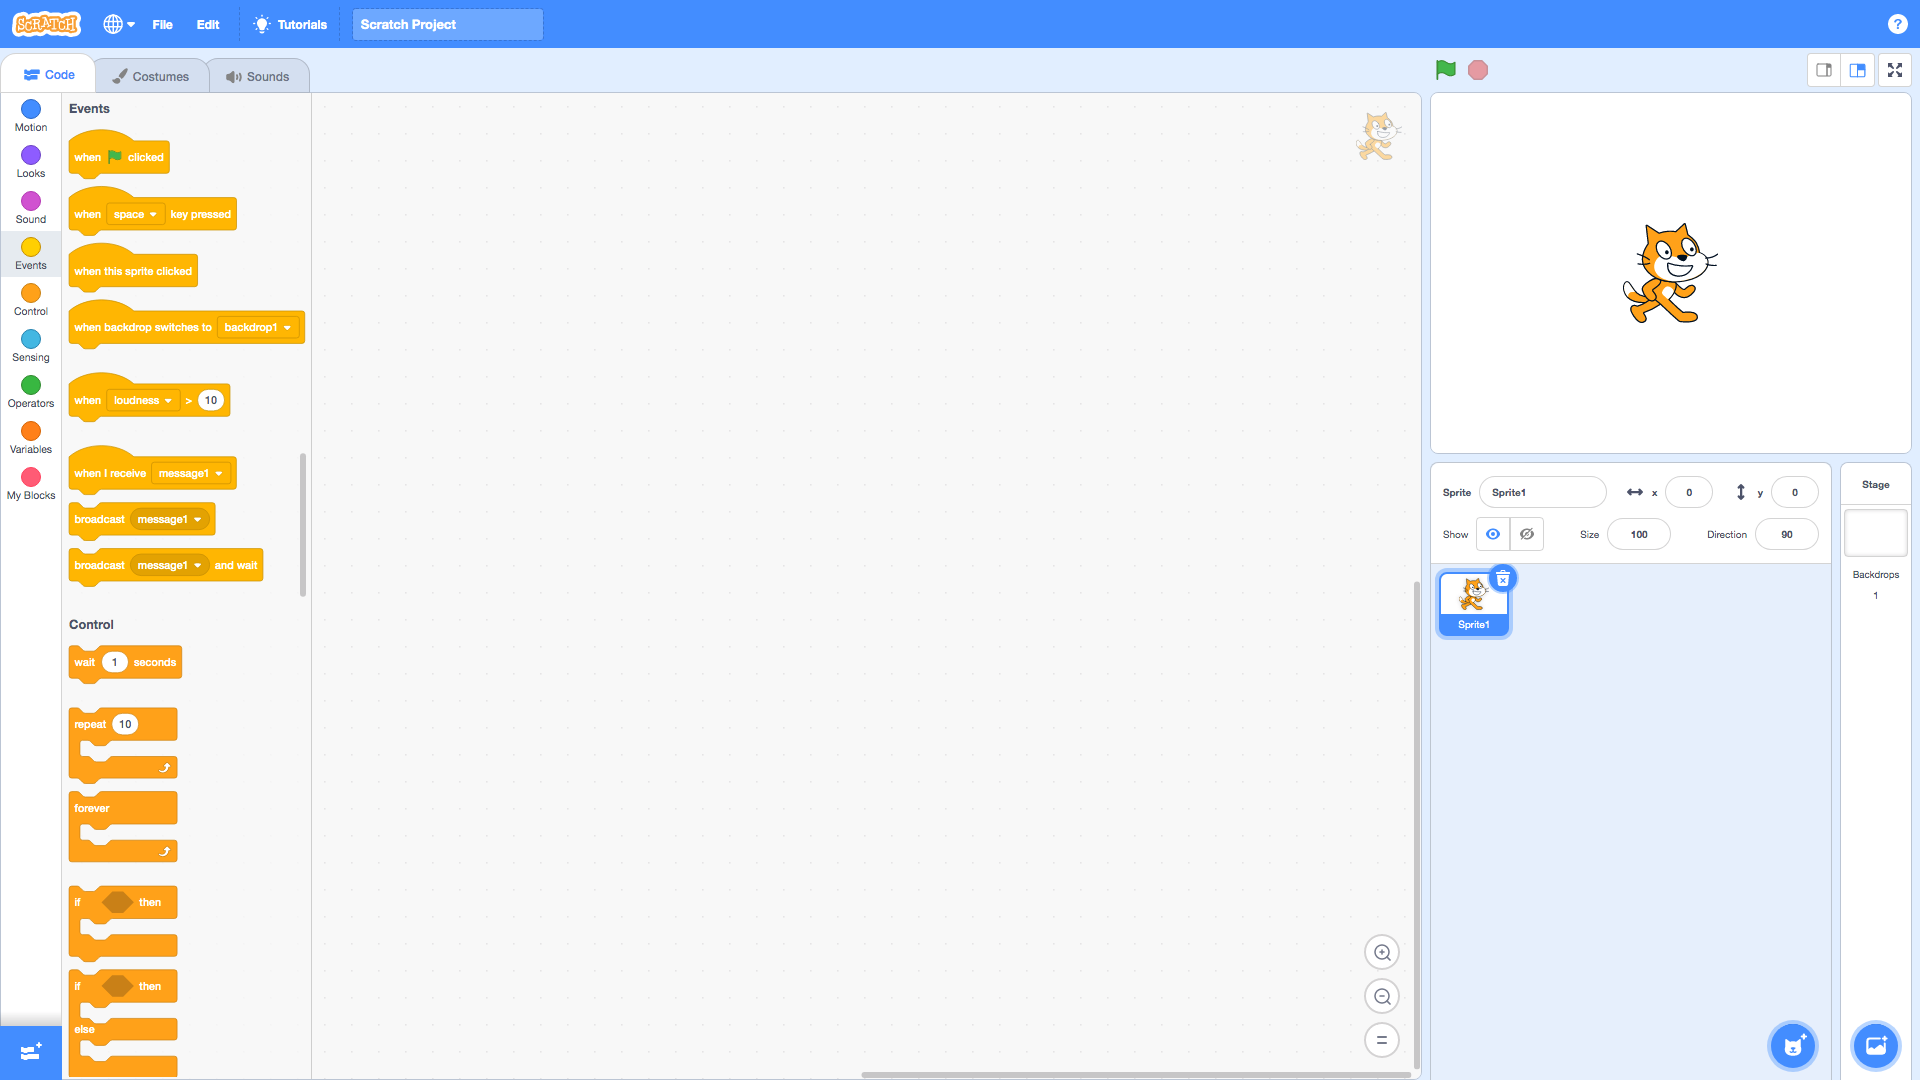
\includegraphics[width=1.0\linewidth,height=0.5\linewidth]{fig020001.png}
   \caption{Grouping instructions}
\label{fig020001}
\end{figure}

The pivotal block in a Scratch program is the one that triggers the execution of the instructions arranged beneath it. This block, known as the "green flag" block (Fig. \ref{fig020002}), determines the initial actions and behaviors when the program is initiated. Upon clicking the green flag, the program springs into action, carrying out the specified sequence of instructions. It serves as the starting point for the program's execution, ensuring that the desired activities and events unfold as intended. By associating instructions with the green flag block, users have control over the program's behavior from the moment it begins running, enabling them to create engaging and interactive experiences.

\begin{figure}[H]
   \centering
   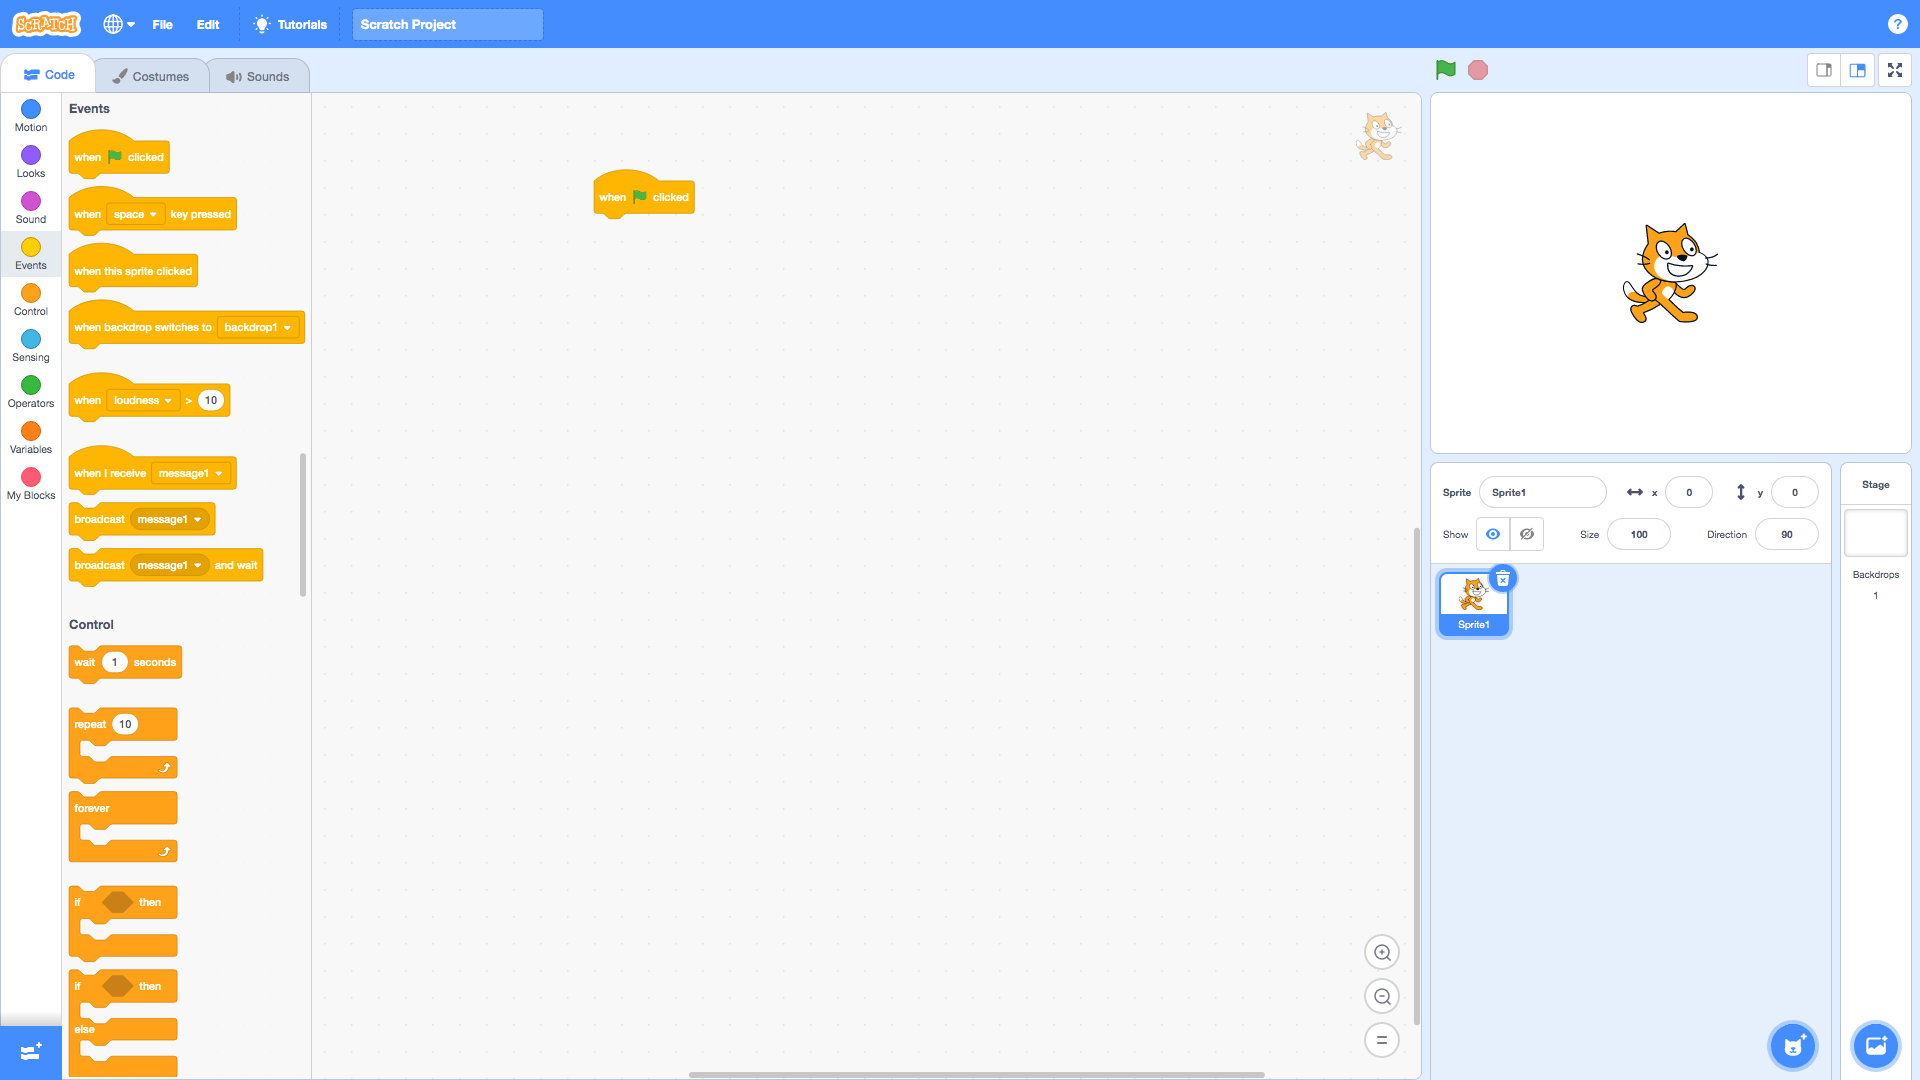
\includegraphics[width=1.0\linewidth,height=0.5\linewidth]{fig020002.png}
   \caption{Starting point of the program}
\label{fig020002}
\end{figure}

The program launch block can be found within the light orange group, specifically designed to respond to user events (Fig. \ref{fig020003}). Unlike traditional programs with a predefined start time, Scratch programs rely on catching user-triggered events to initiate their execution. This flexible approach allows users to determine when they want their program to begin running.

Similarly, the second crucial block, located within the dark orange group, is responsible for ending the program's execution (Fig. \ref{fig020003}). Users can halt all ongoing processes by utilizing this block and bringing the program to a controlled stop. It ensures that any actions, animations, or events running in the program come to a complete halt, allowing for a smooth and controlled termination. This block's availability will enable users to define their programs' desired duration and behavior, enhancing their control and facilitating a more refined user experience.

\begin{figure}[H]
   \centering
   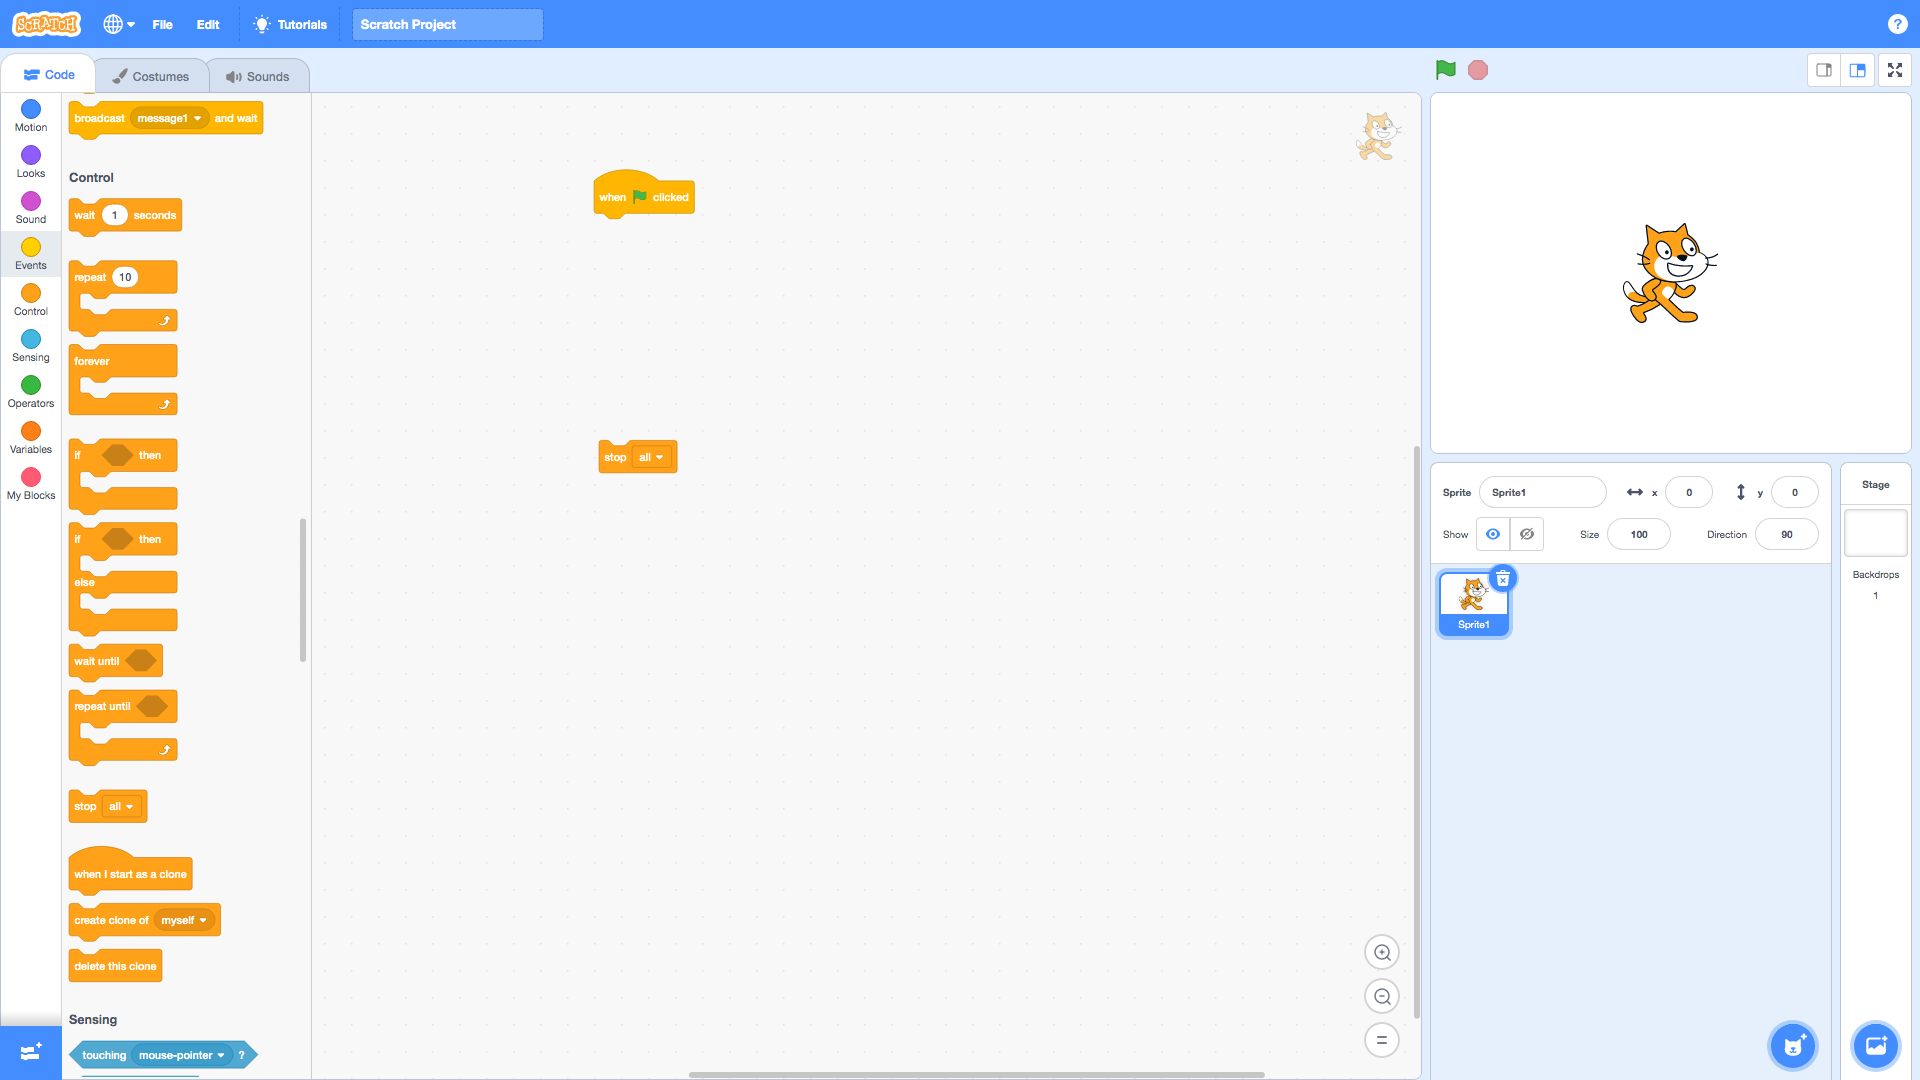
\includegraphics[width=1.0\linewidth,height=0.5\linewidth]{fig020003.png}
   \caption{Program endpoint}
\label{fig020003}
\end{figure}

The dark orange group encompasses performance control blocks, which play a crucial role in determining the program's flow and enabling the repetition of a group of actions.

In Scratch, the instruction blocks primarily govern the behavior of graphical elements known as sprites. Unlike static computer images, sprites are dynamic graphic objects with multiple frames depicting the character in various configurations. Creating a new Scratch program automatically begins with a single sprite, represented by the iconic orange cat, positioned at coordinates (x=0, y=0). The Scratch workspace utilizes a two-dimensional coordinate system centered at (0,0), providing a framework for positioning and manipulating sprites within a visual environment.

\begin{figure}[H]
   \centering
   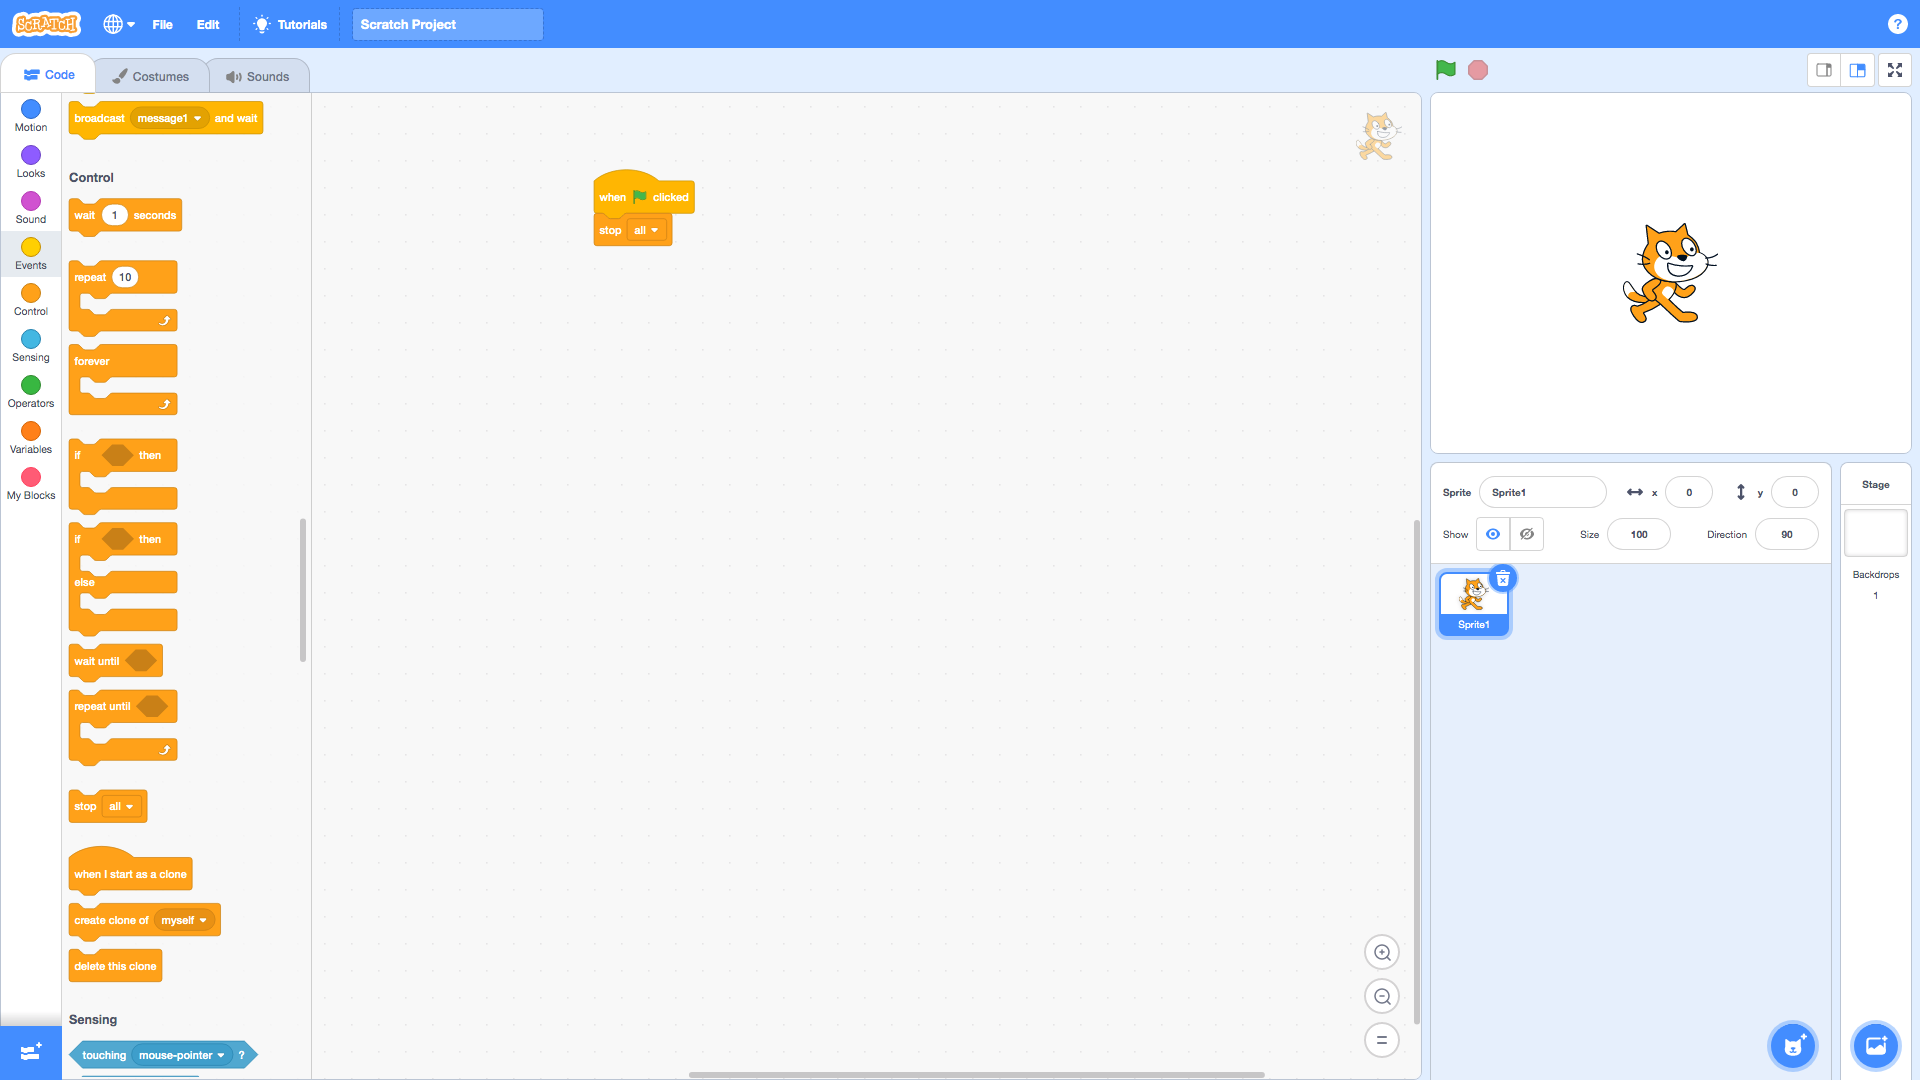
\includegraphics[width=1.0\linewidth,height=0.5\linewidth]{fig020004.png}
   \caption{Finish immediately after starting}
\label{fig020004}
\end{figure}

When the start and end blocks are connected (Fig. \ref{fig020004}), the program becomes idle and performs no actions. It terminates as soon as it starts, rendering it purposeless. The blocks in the blue group come into play to initiate meaningful actions. The initial block commands the cat sprite to move precisely 10 steps, and this value can be customized by inserting a different number within the block (Fig. \ref{fig020005}).

\begin{figure}[H]
   \centering
   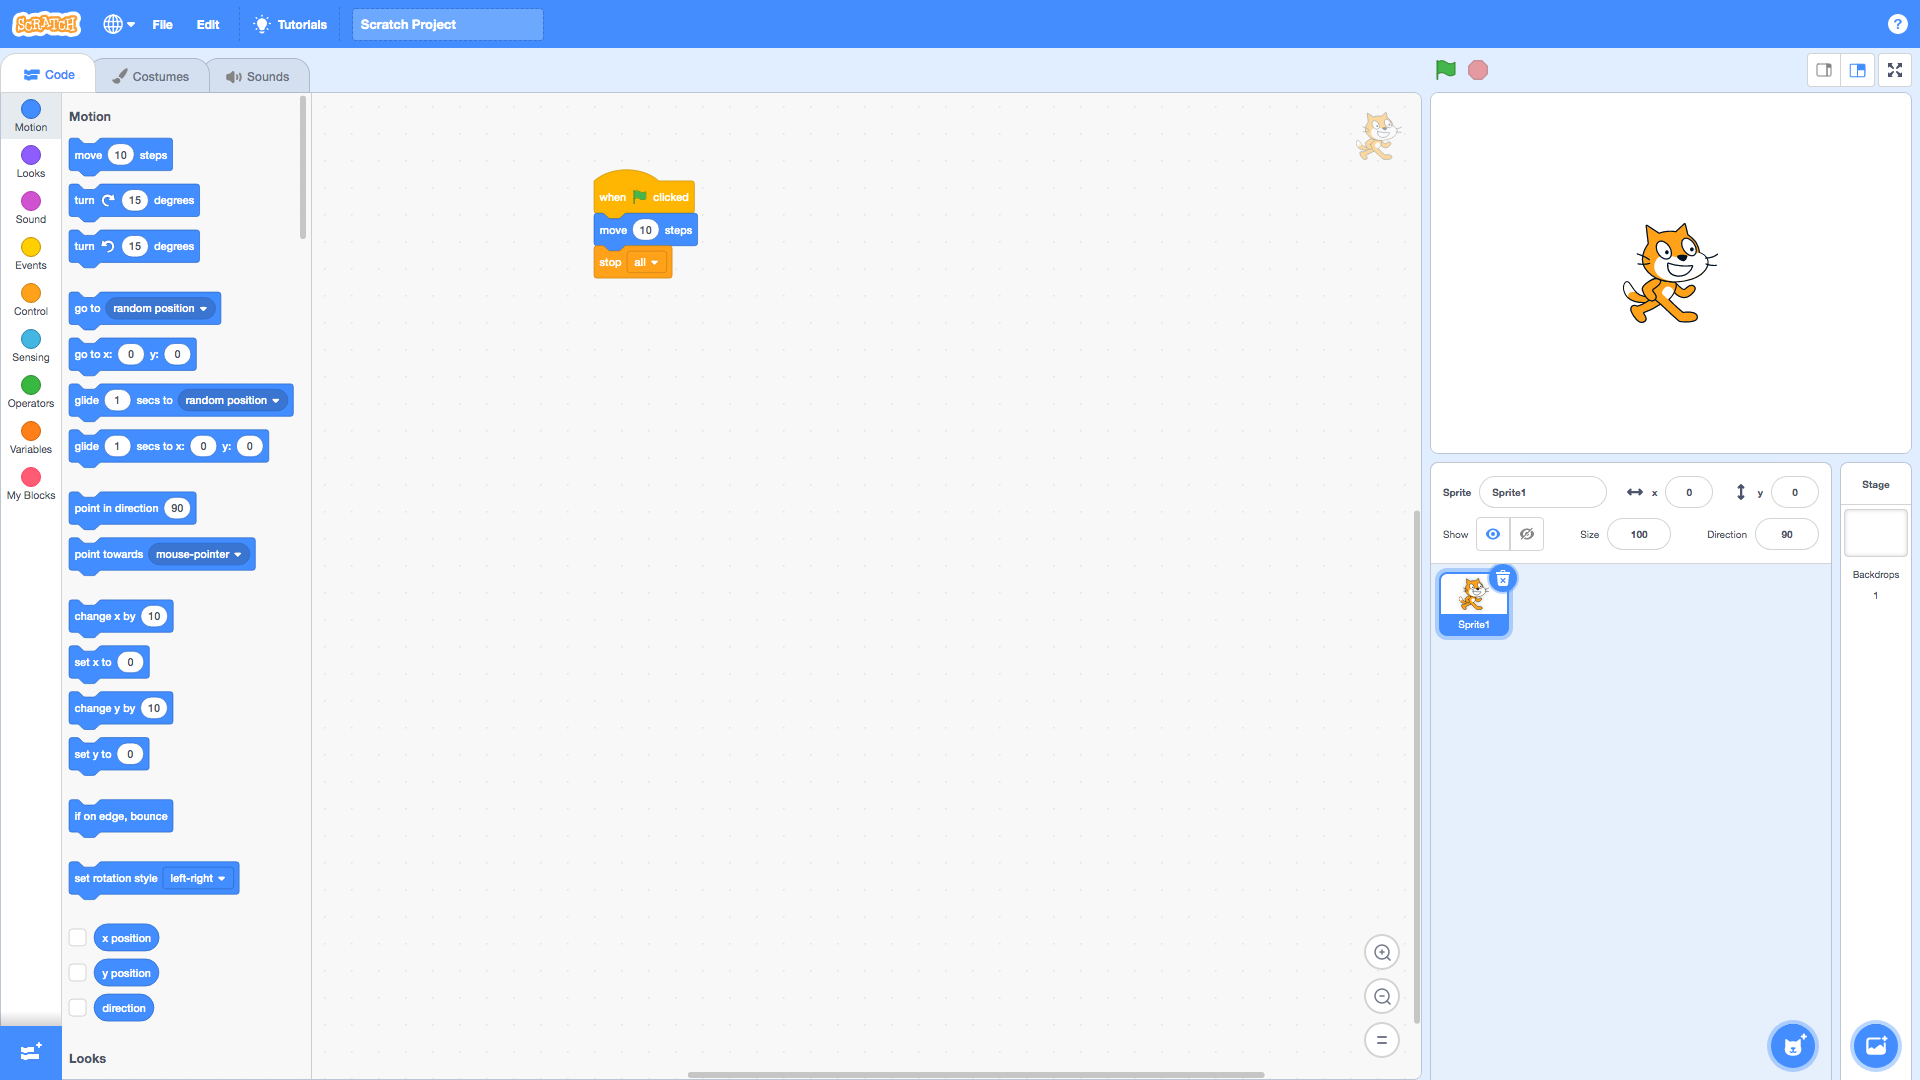
\includegraphics[width=1.0\linewidth,height=0.5\linewidth]{fig020005.png}
   \caption{Moving Character}
\label{fig020005}
\end{figure}

The subsequent block in the group directs the character to rotate a specific number of degrees in a clockwise direction relative to its center (Fig. \ref{fig020006}).

\begin{figure}[H]
   \centering
   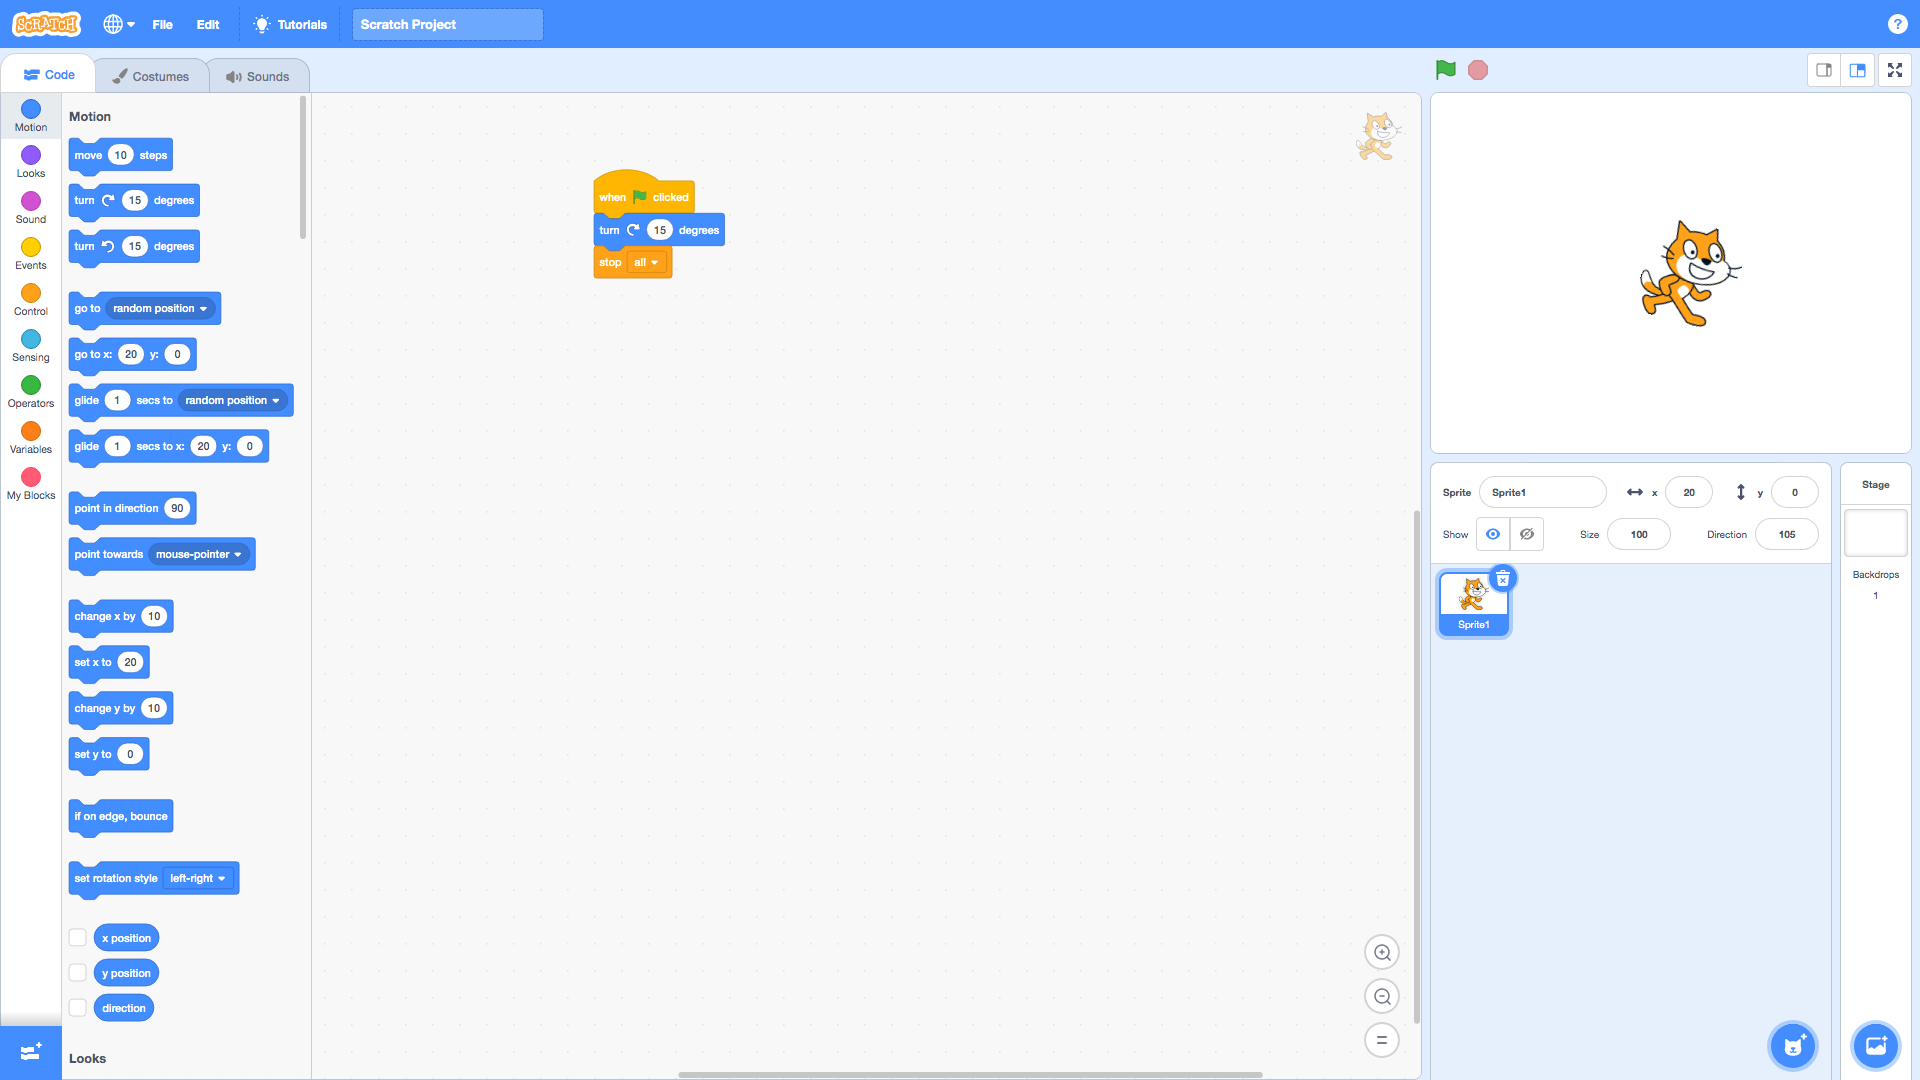
\includegraphics[width=1.0\linewidth,height=0.5\linewidth]{fig020006.png}
   \caption{Clockwise Rotation}
\label{fig020006}
\end{figure}

Similarly, the next block in the group allows the rotation to be performed counterclockwise (Fig. \ref{fig020007}).

\begin{figure}[H]
   \centering
   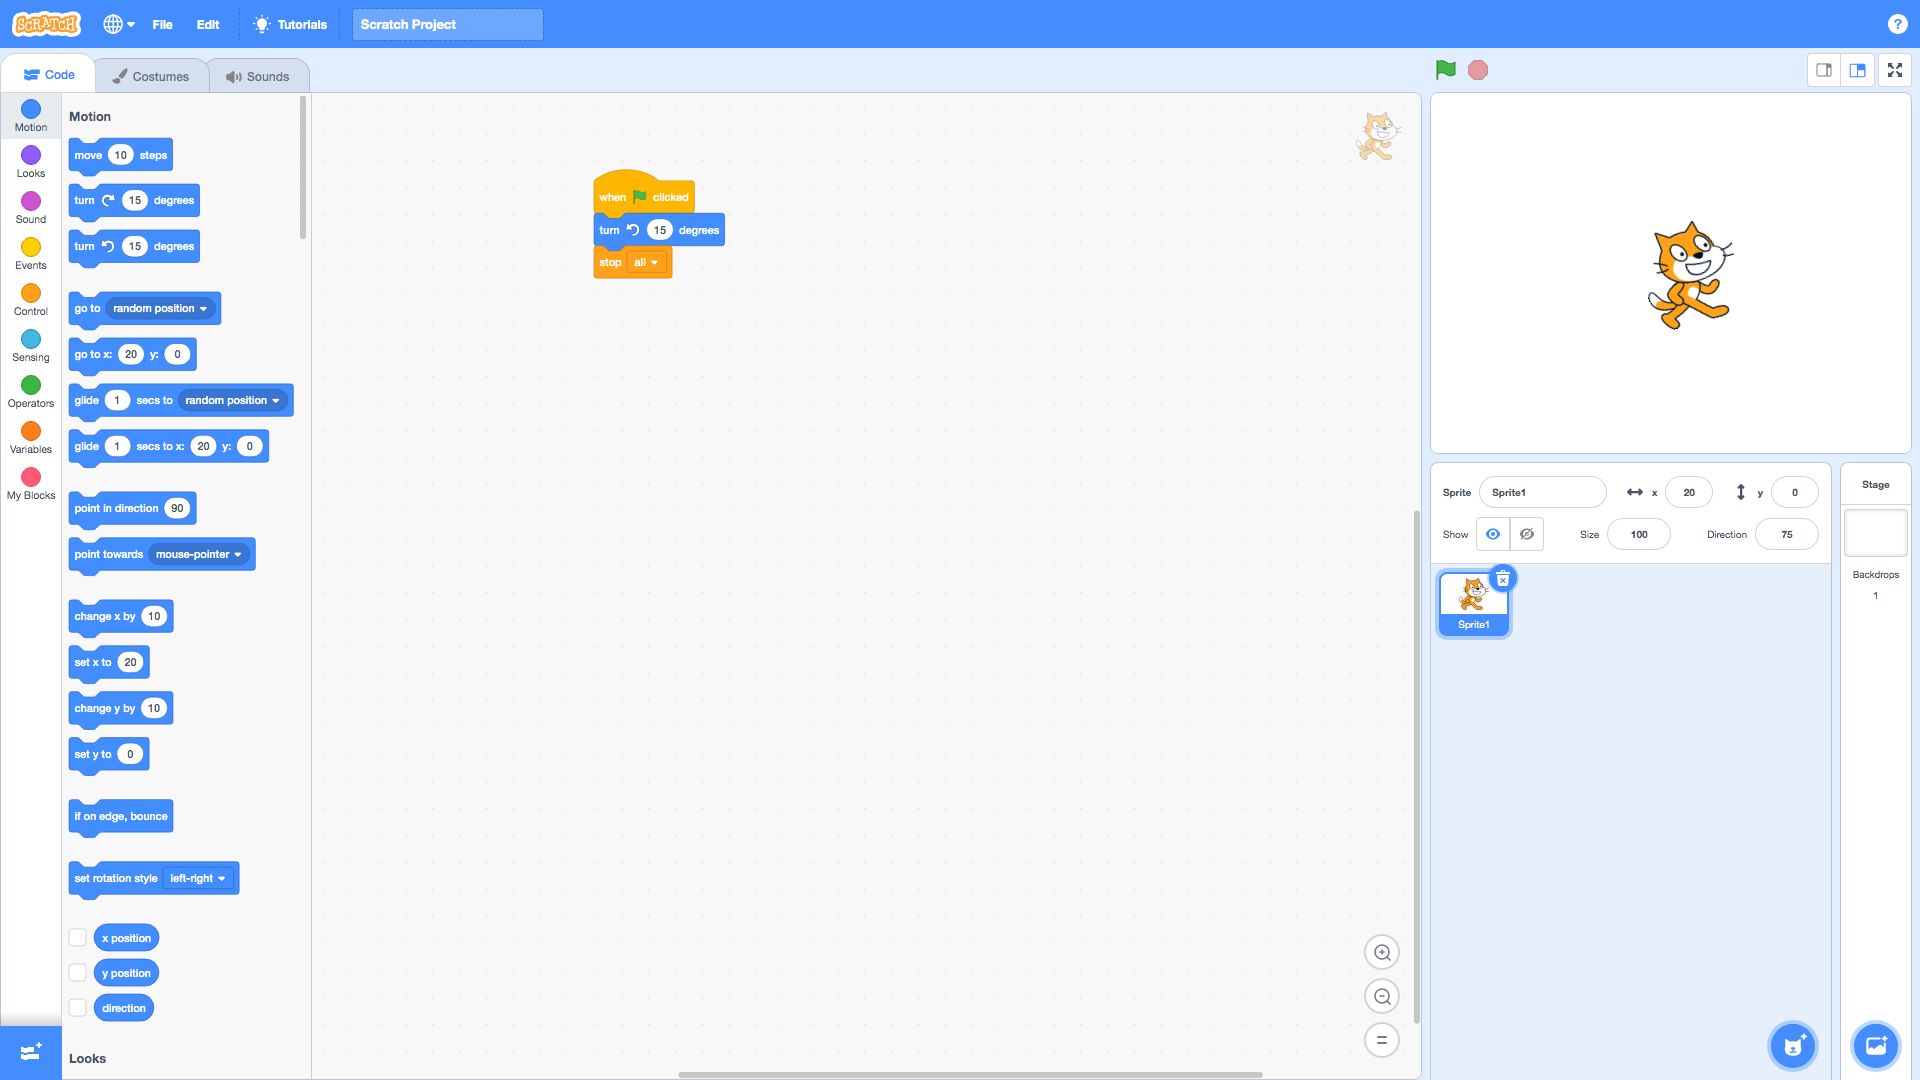
\includegraphics[width=1.0\linewidth,height=0.5\linewidth]{fig020007.png}
   \caption{Counterclockwise rotation}
\label{fig020007}
\end{figure}

The next block in the group allows the character to move to random coordinates or coordinates specified with the mouse (Fig. \ref{fig020008}).

\begin{figure}[H]
   \centering
   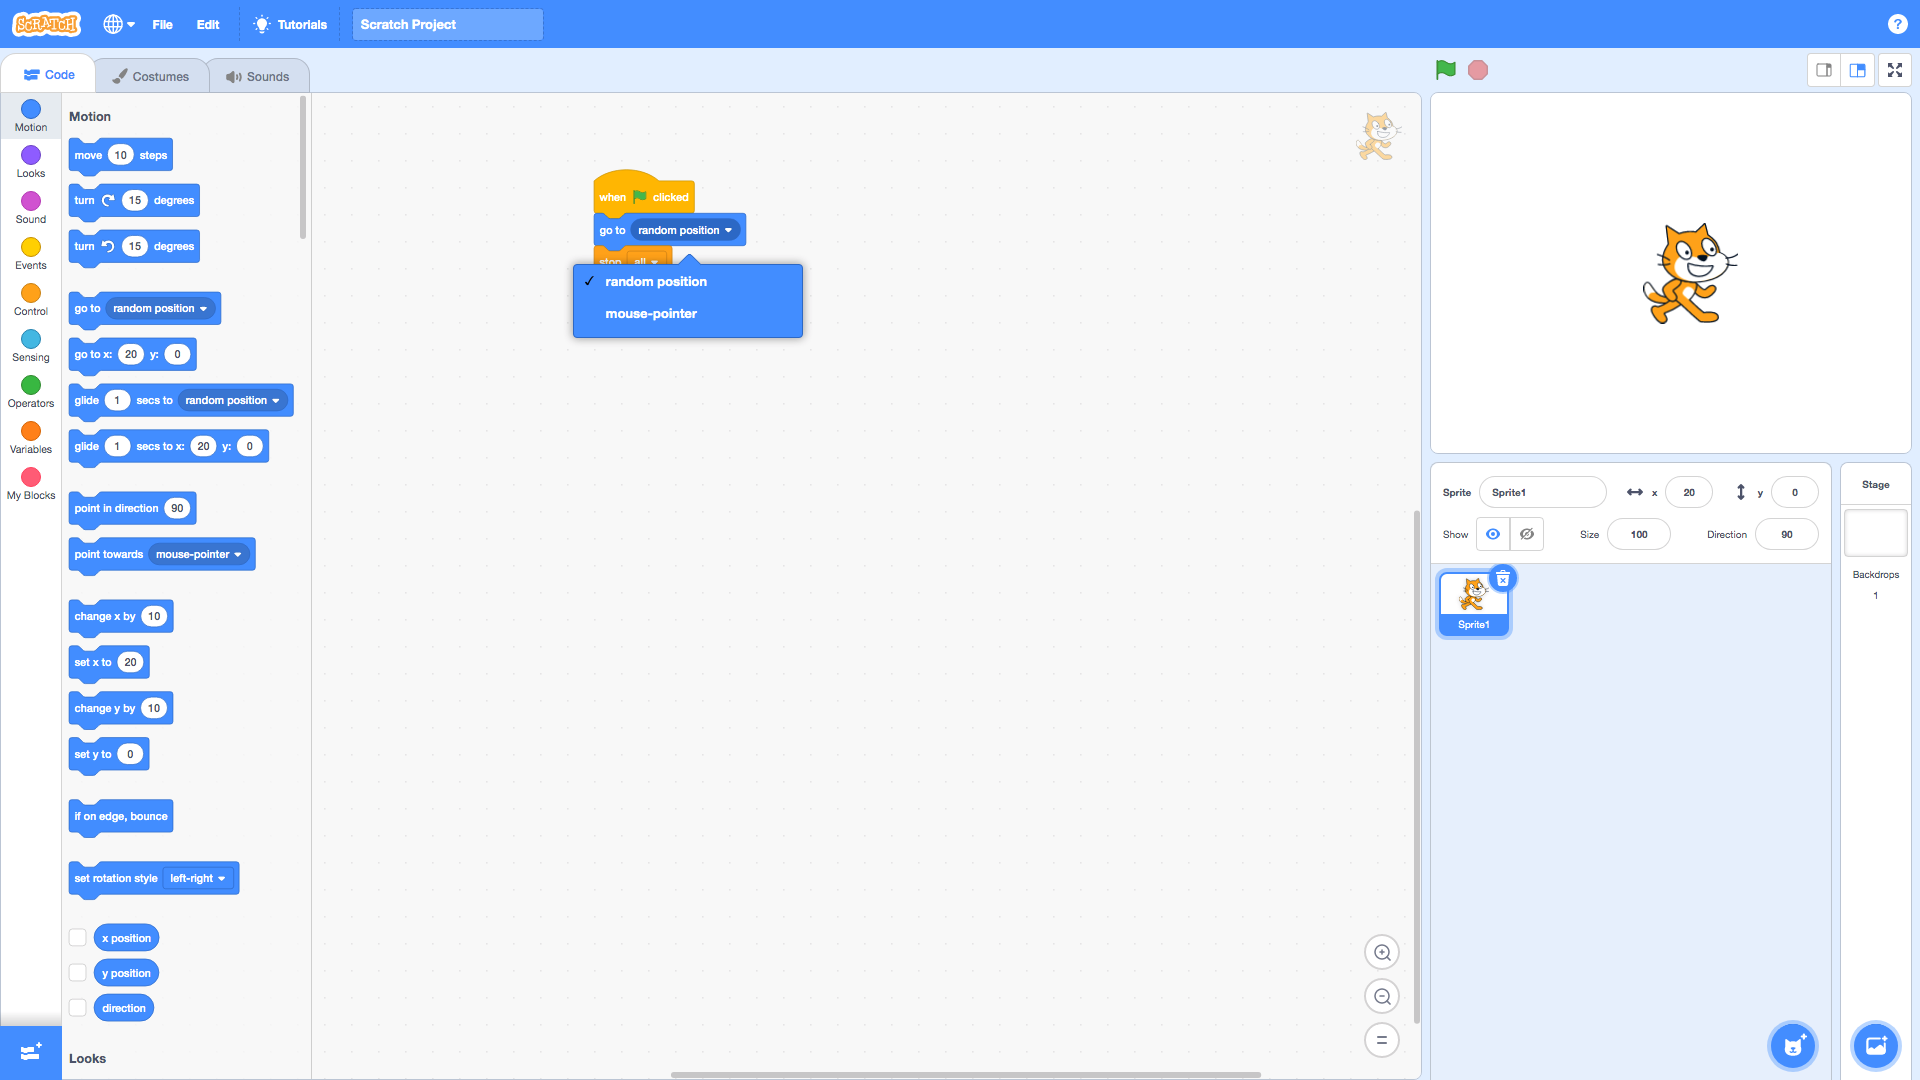
\includegraphics[width=1.0\linewidth,height=0.5\linewidth]{fig020008.png}
   \caption{Move to random position}
\label{fig020008}
\end{figure}

The movement of the character can also be set by absolute coordinates using a block that allows entering numbers for the x-axis (abscissa) and y-axis (ordinate) (Fig. \ref{fig020009}).

\begin{figure}[H]
   \centering
   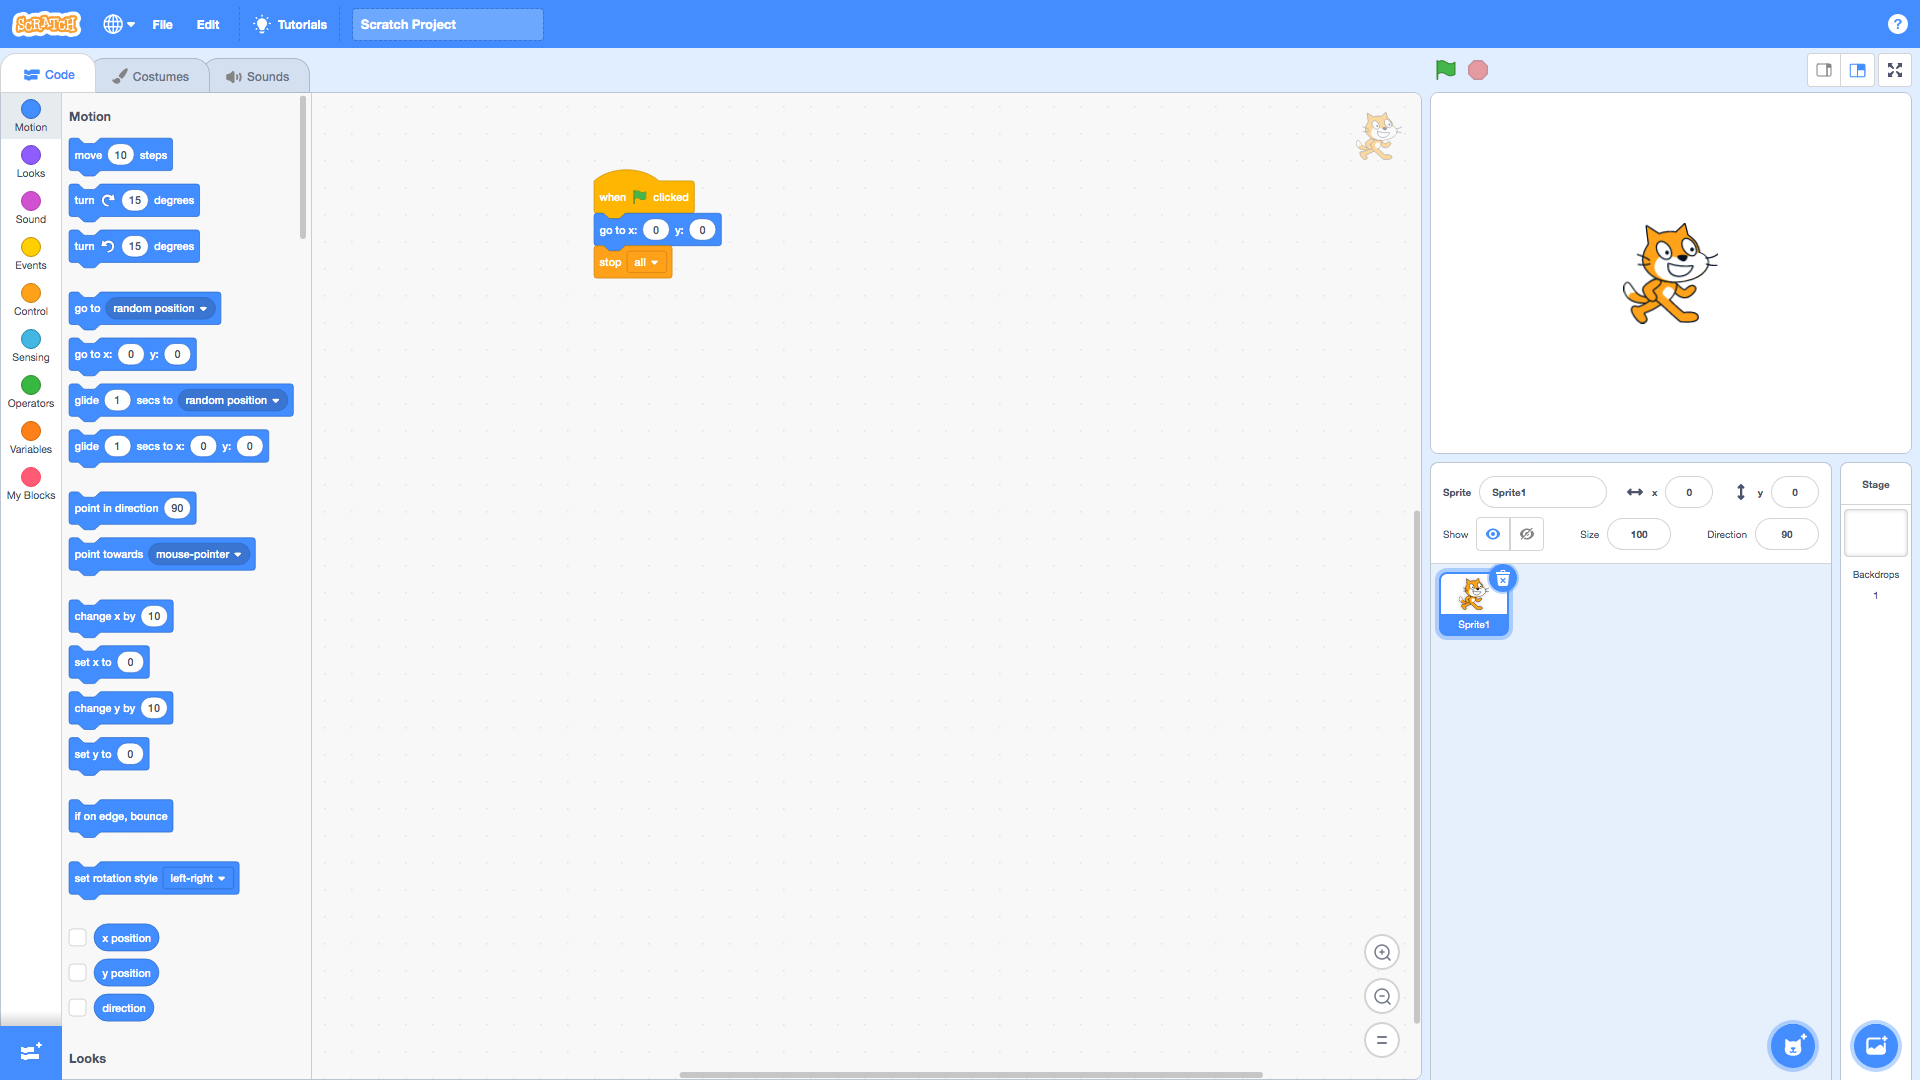
\includegraphics[width=1.0\linewidth,height=0.5\linewidth]{fig020009.png}
   \caption{Move by absolute coordinates}
\label{fig020009}
\end{figure}

Smooth movement at a predetermined time interval to random coordinates or coordinates specified by the mouse is possible with the next block in the group (Fig. \ref{fig020010}).

\begin{figure}[H]
   \centering
   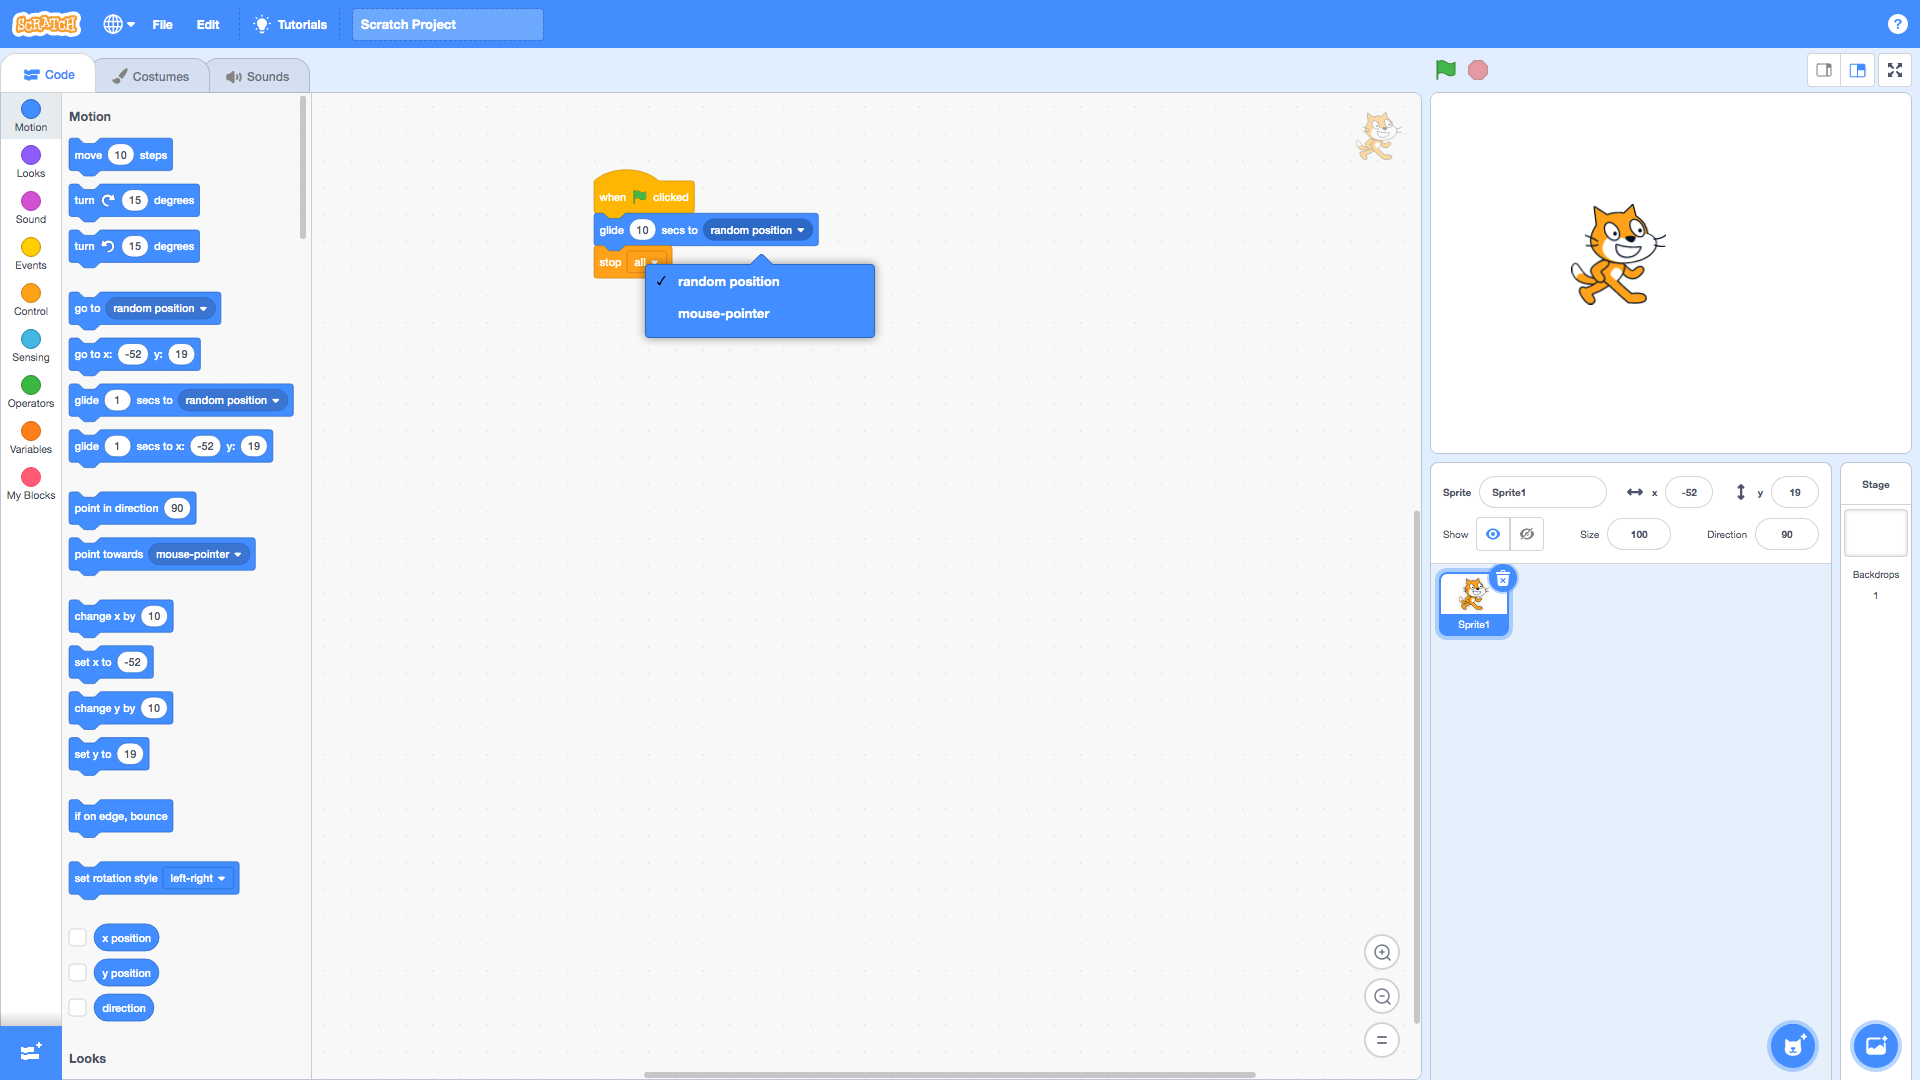
\includegraphics[width=1.0\linewidth,height=0.5\linewidth]{fig020010.png}
   \caption{Slide to random position}
\label{fig020010}
\end{figure}

Smooth sliding to predetermined coordinates for a predetermined time interval is possible with the block specifically designed for this purpose (Fig. \ref{fig020011}).

\begin{figure}[H]
   \centering
   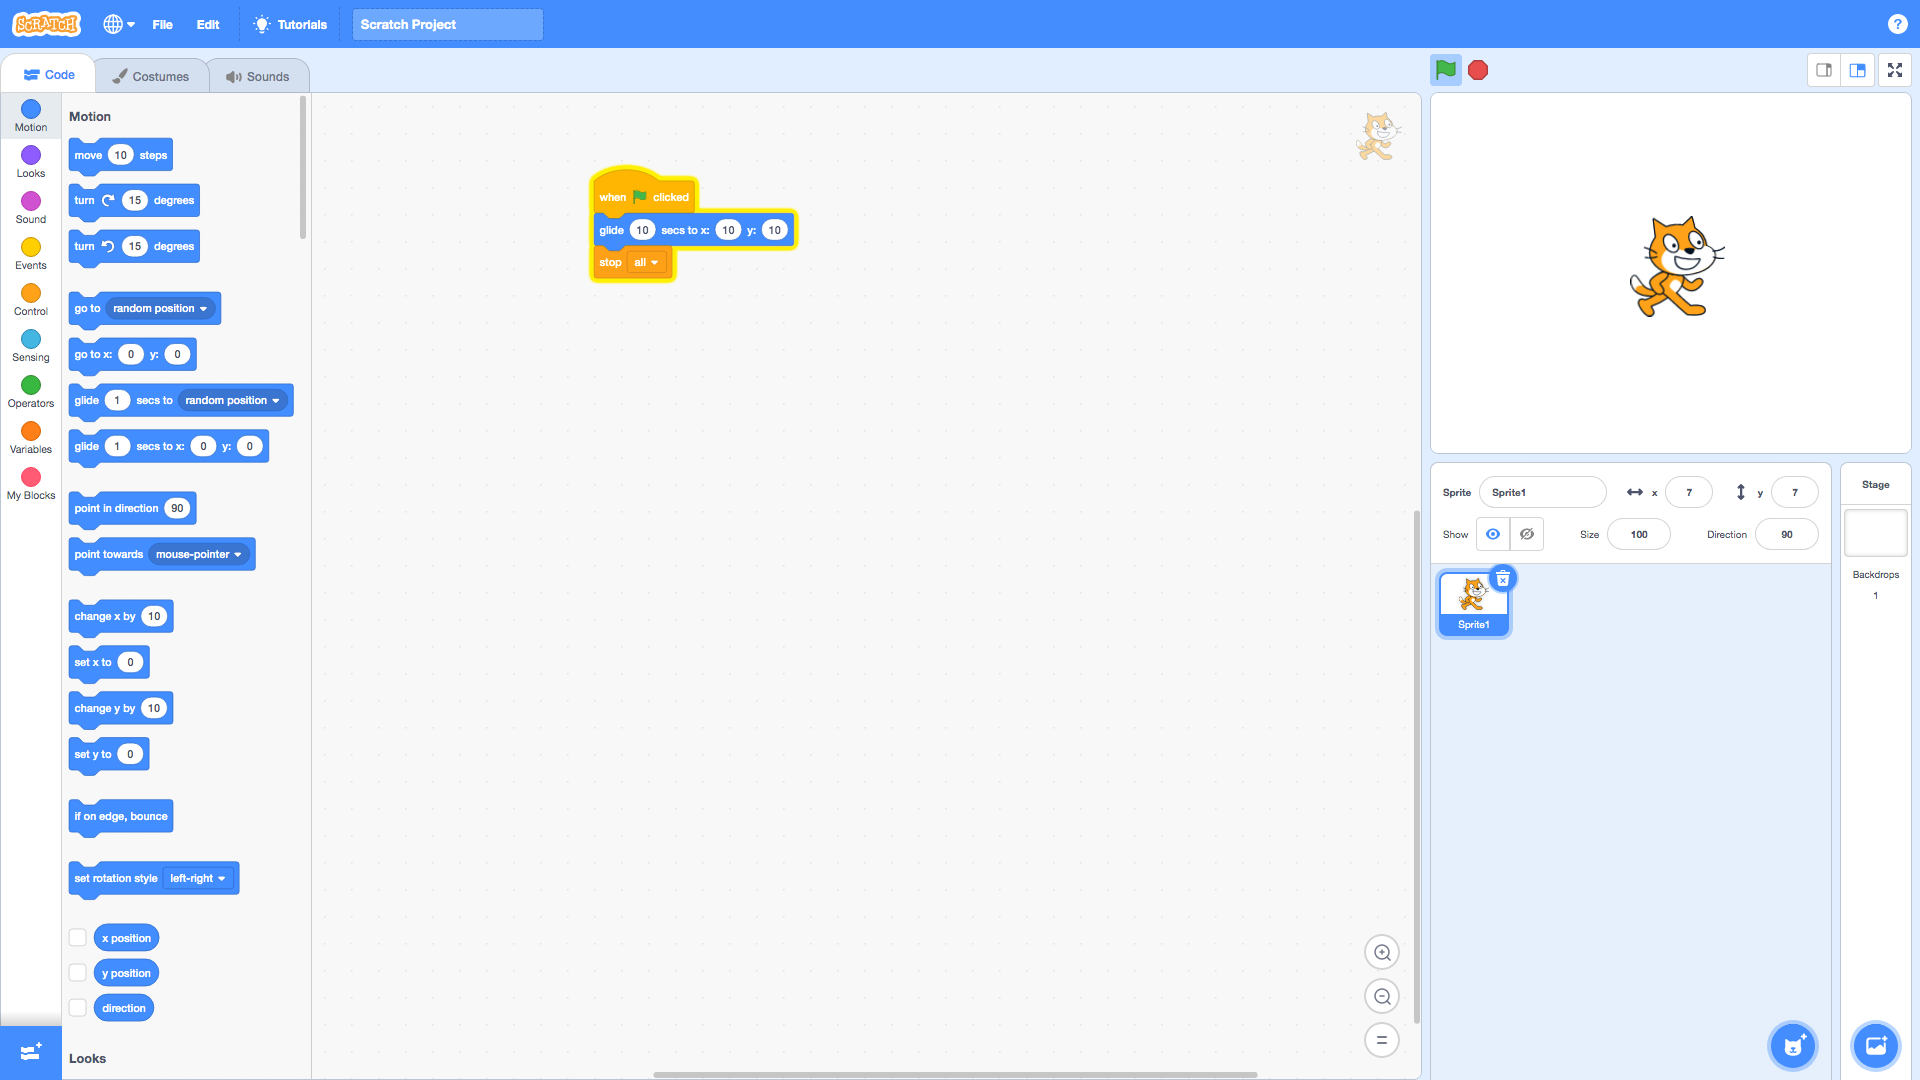
\includegraphics[width=1.0\linewidth,height=0.5\linewidth]{fig020011.png}
   \caption{Slide to set coordinates}
\label{fig020011}
\end{figure}

To change the orientation of the animated character, which is represented by an angle, a block is used that allows you to specify a specific angle (Fig. \ref{fig020012}). This angle determines the direction the character is facing, with 90 degrees representing the rightward direction for the orange cat sprite.

\begin{figure}[H]
   \centering
   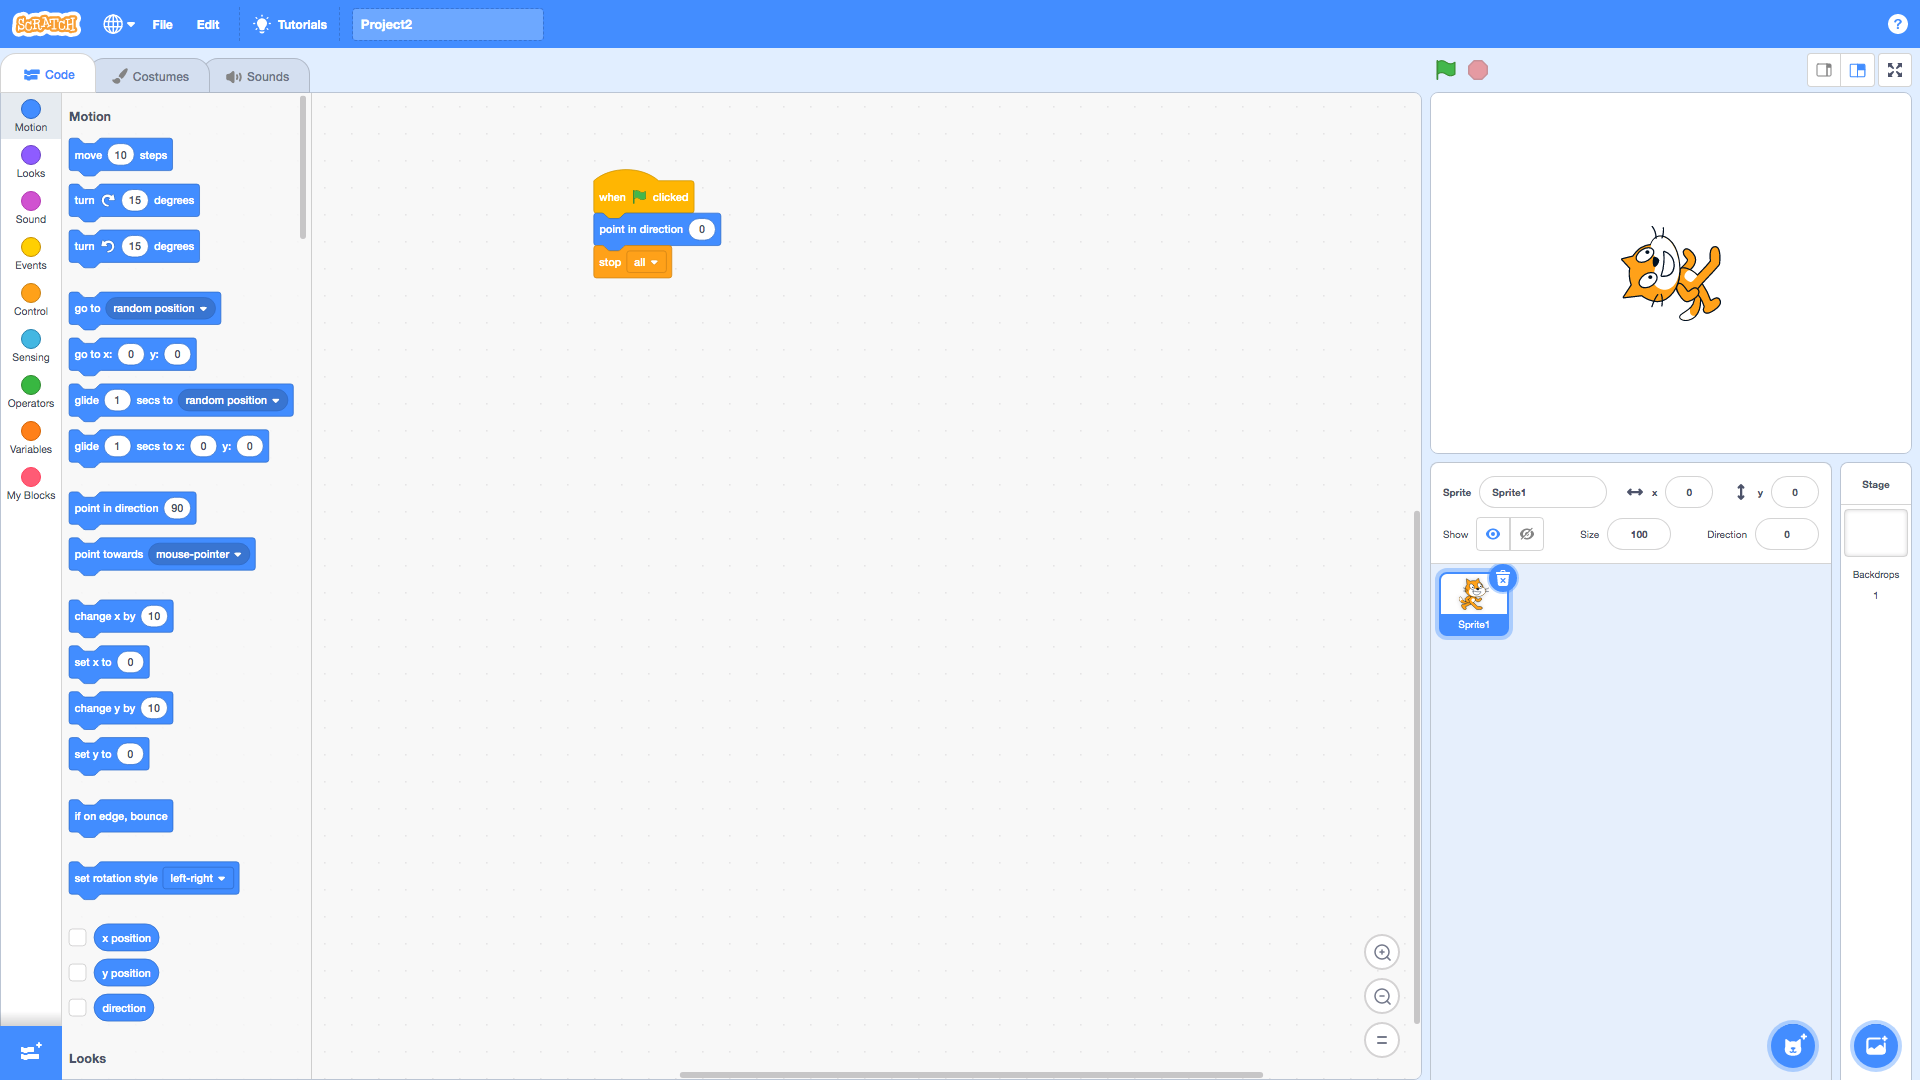
\includegraphics[width=1.0\linewidth,height=0.5\linewidth]{fig020012.png}
   \caption{Corner Orientation}
\label{fig020012}
\end{figure}

In more complex character control scenarios, there are instances where the character needs to track the movement of the mouse pointer. To achieve this, Scratch provides a specific block that executes this instruction (Fig. \ref{fig020013}). Using this block, the character's position will be updated to match the current position of the mouse pointer.

\begin{figure}[H]
   \centering
   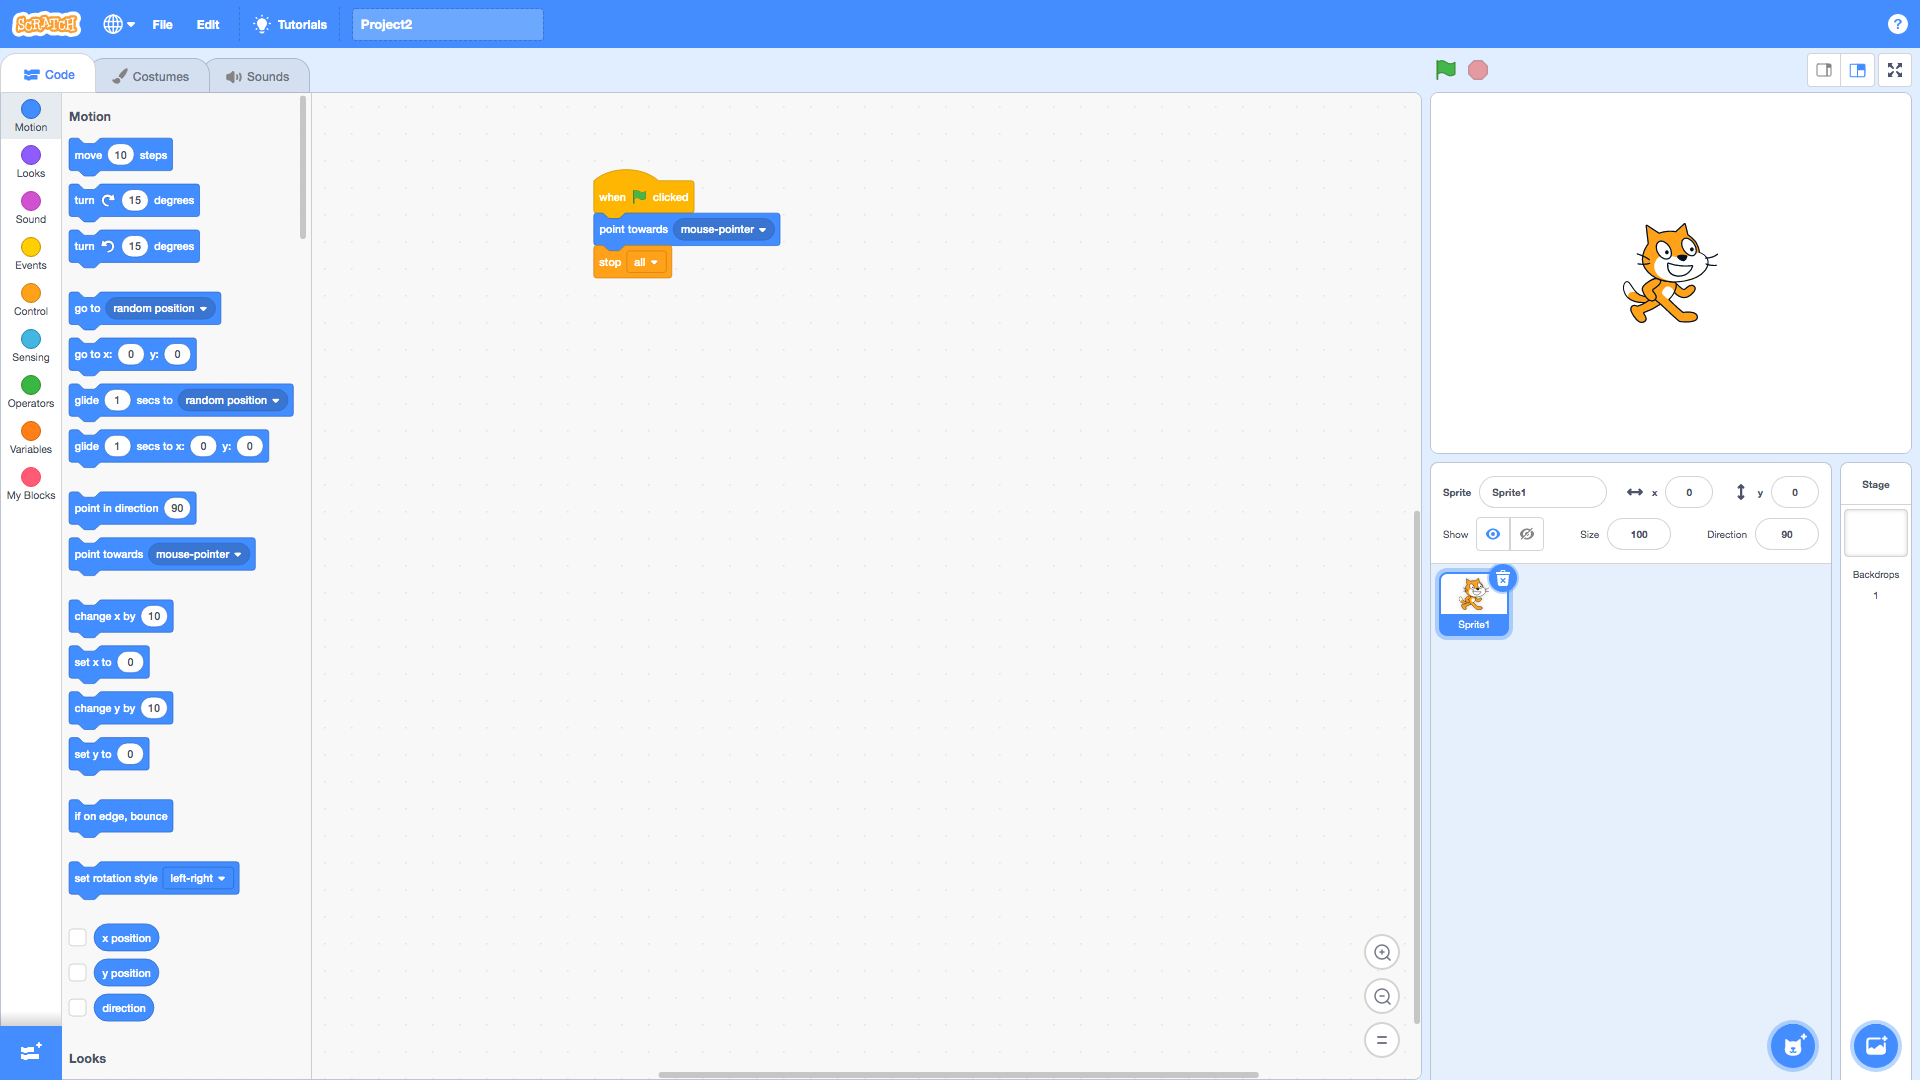
\includegraphics[width=1.0\linewidth,height=0.5\linewidth]{fig020013.png}
   \caption{Mouse Pointer Orientation}
\label{fig020013}
\end{figure}

Blocks can be arranged sequentially, allowing for sequential changes in the character's relative x and y coordinates. Scratch provides specific blocks for this purpose (Fig. \ref{fig020014}). These blocks enable you to move the character's position by a specified amount in the x and y directions relative to its current position. Combining these blocks in a sequence allows you to create complex movement patterns for the character.

\begin{figure}[H]
   \centering
   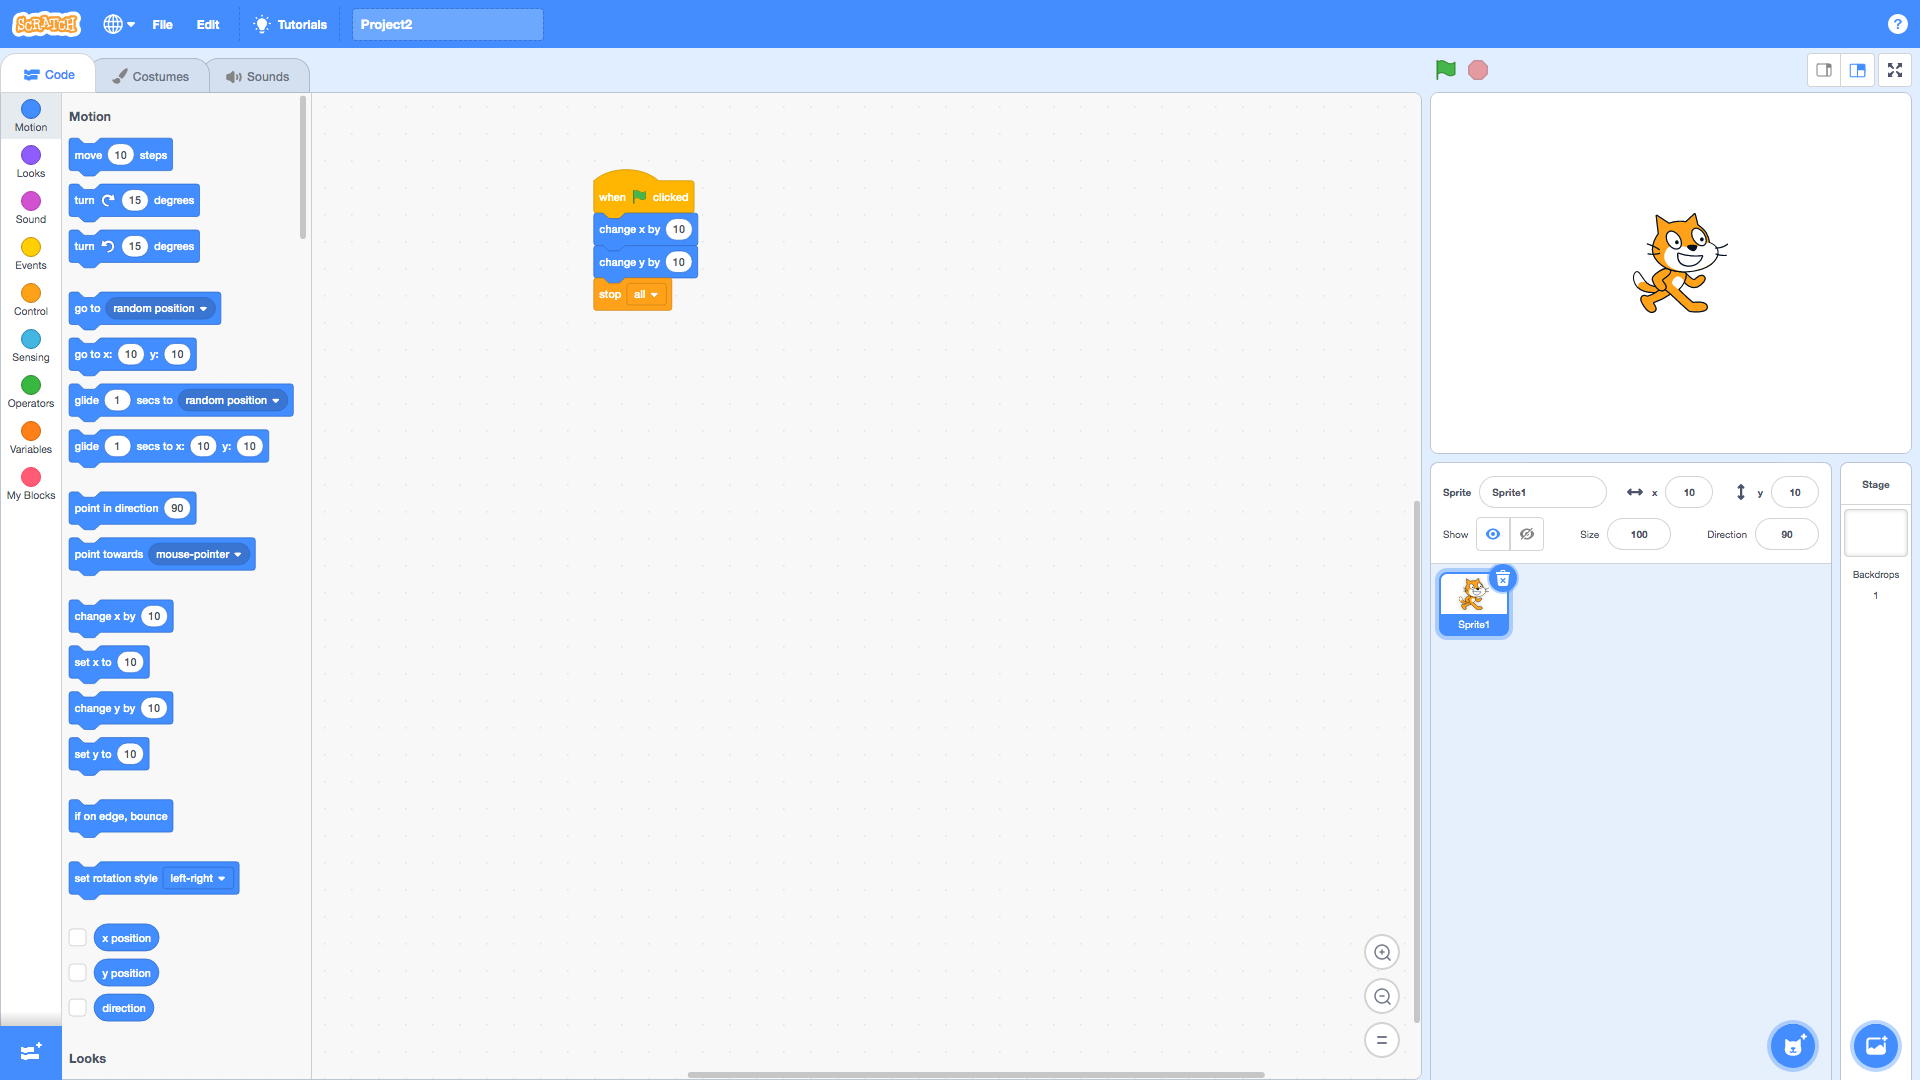
\includegraphics[width=1.0\linewidth,height=0.5\linewidth]{fig020014.png}
   \caption{Sequential change of relative coordinates}
\label{fig020014}
\end{figure}

In addition to relative changes in coordinates, Scratch allows for absolute changes in coordinates. The absolute change is relative to the center of the coordinate system. Using the appropriate blocks (Fig. \ref{fig020015}), you can specify the exact x and y coordinates where you want the character to move, regardless of its current position. This provides precise control over the character's placement on the stage.

\begin{figure}[H]
   \centering
   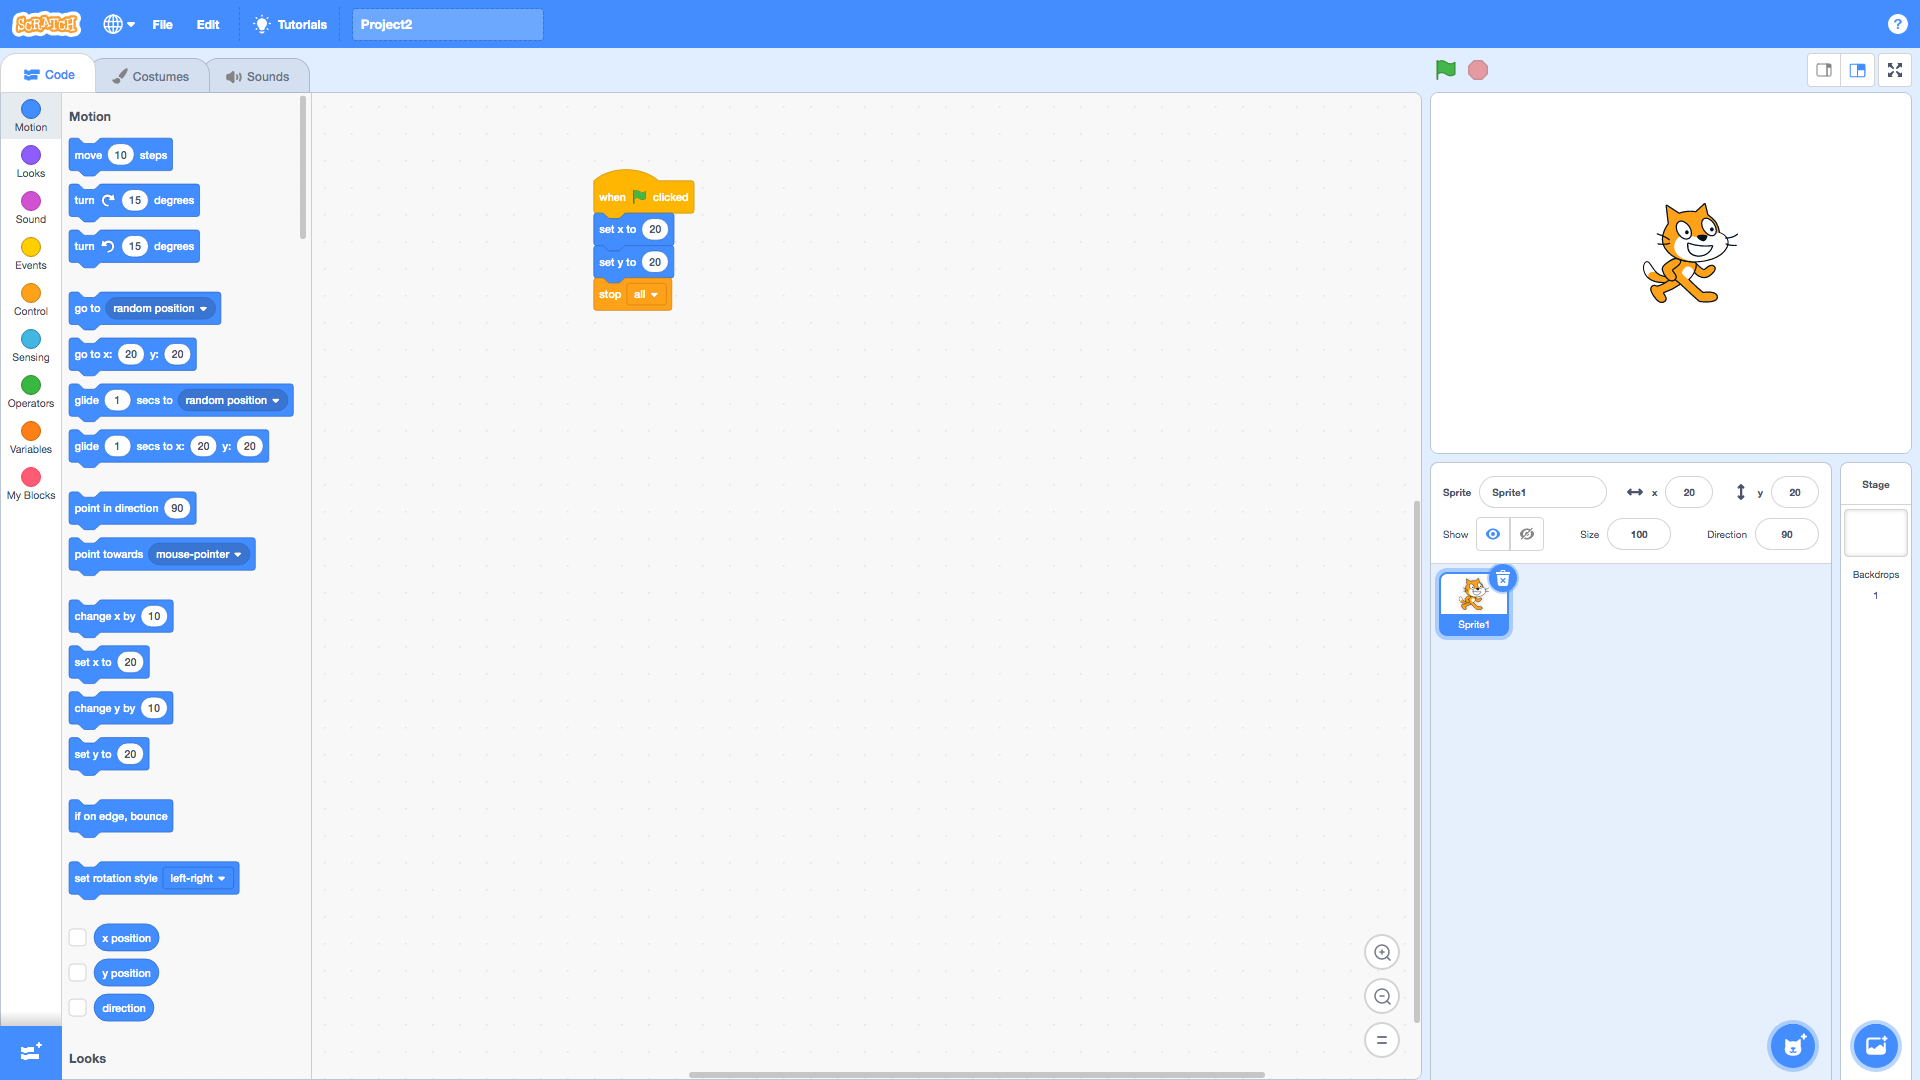
\includegraphics[width=1.0\linewidth,height=0.5\linewidth]{fig020015.png}
   \caption{Sequential change of absolute coordinates}
\label{fig020015}
\end{figure}

Different options are available to handle the animated character's movement when it reaches the boundaries of the workspace in Scratch. One option is to allow the character to continue moving outside the visible area. However, another option is to make the character bounce off the edges of the workspace. This can be achieved using a specific block designed for this purpose (Fig. \ref{fig020016}).

Implementing the bounce behavior requires a slightly more complex sequence of instructions. Each time the program is run, the relative coordinates of the character are changed first, and then an edge bounce is performed if necessary. A green block is utilized to add some variability to the scenario instead of using fixed relative offset values. This green block allows generating of a random number within a predetermined range. It's worth noting that the green block has an oval shape, indicating that it is meant to fit into one of the other blocks with an oval slot.

Incorporating the edge bounce block and random number generation can create more dynamic and interactive movement patterns for your animated character within the Scratch environment.

\begin{figure}[H]
   \centering
   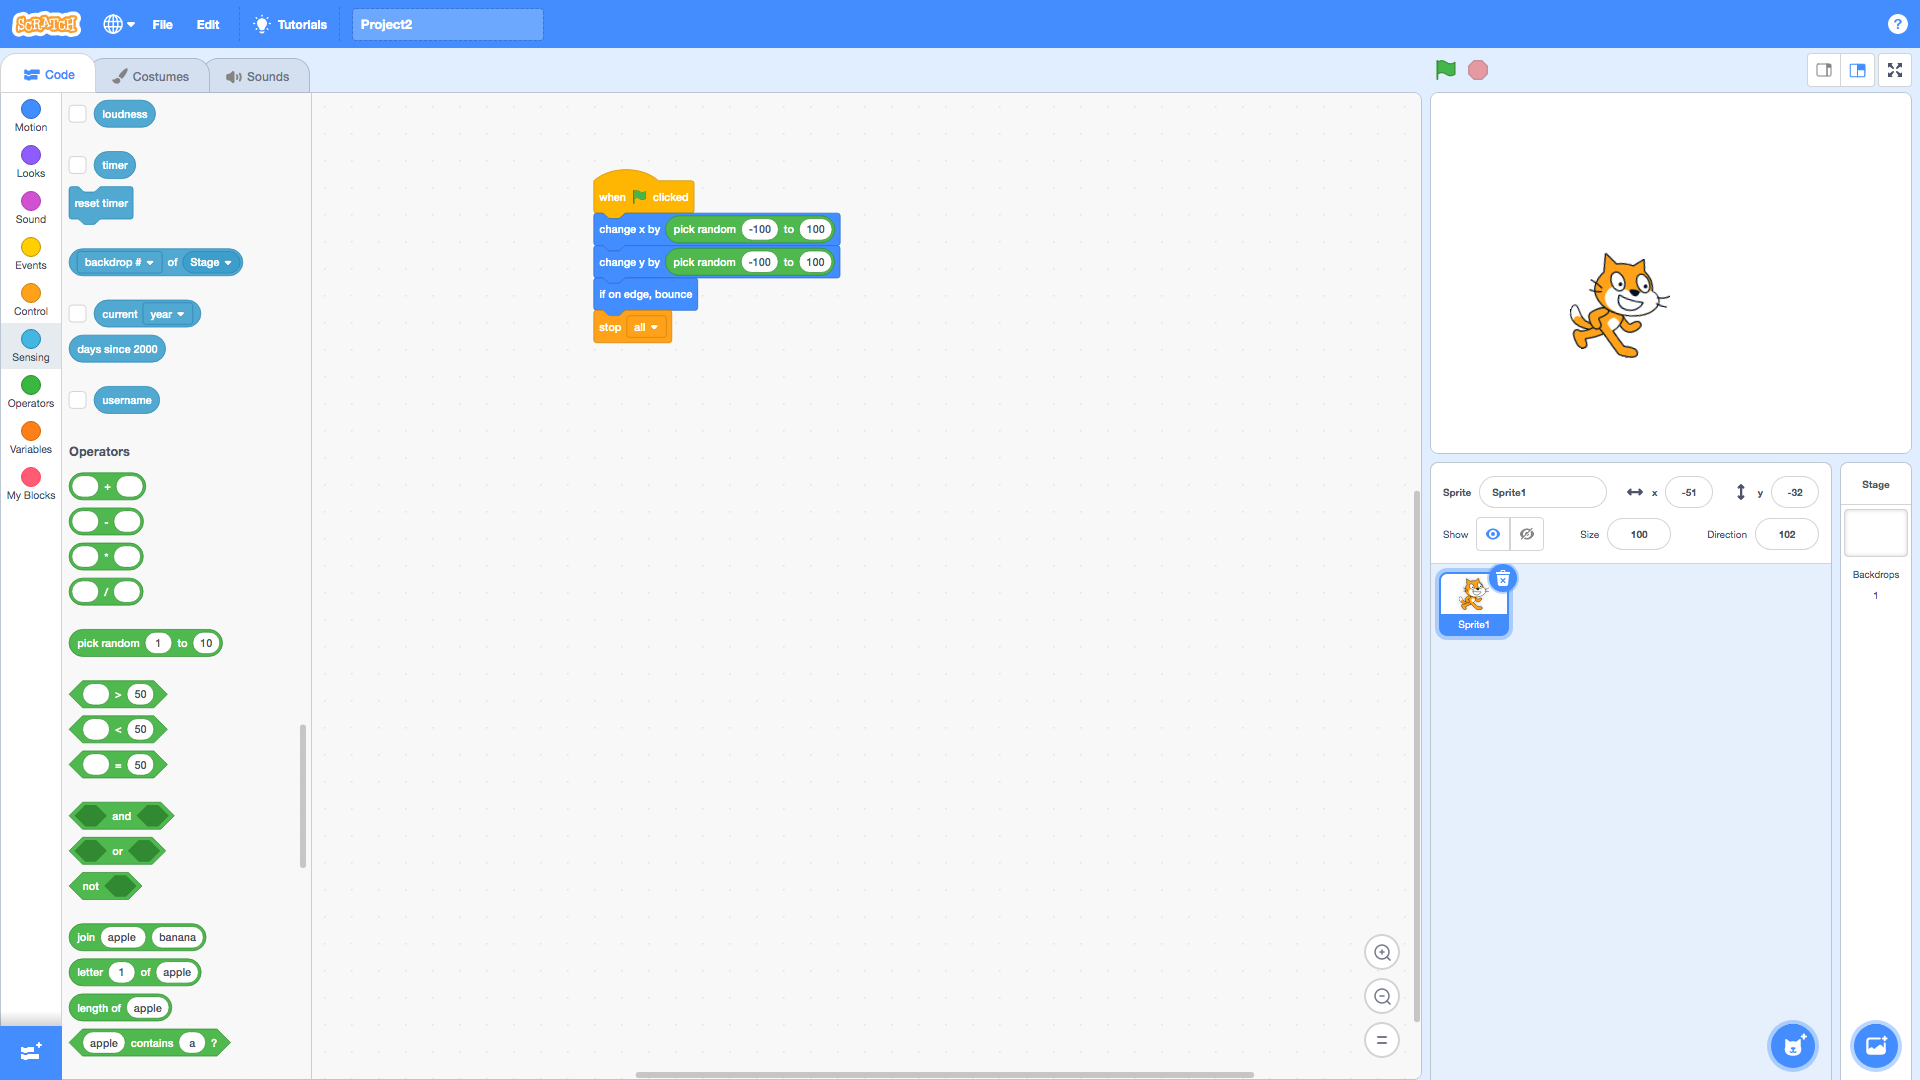
\includegraphics[width=1.0\linewidth,height=0.5\linewidth]{fig020016.png}
   \caption{Bouncing off the edges}
\label{fig020016}
\end{figure}

Another essential block from the dark orange group is the "wait" block, which allows you to introduce delays in your program (Fig. \ref{fig020017}). By placing this block between the start and end blocks, you can instruct the program to pause for a specified number of seconds before proceeding with the subsequent instructions. While the program is executing, you will notice a yellow frame around the sequence of instructions, indicating that the program is running those blocks.

The "wait" block is handy when you want to introduce timing or create pauses in the execution of your program. It allows for better control over the instructions flow and can be used to synchronize actions, create delays between movements, or add timing-related effects to your project.

\begin{figure}[H]
   \centering
   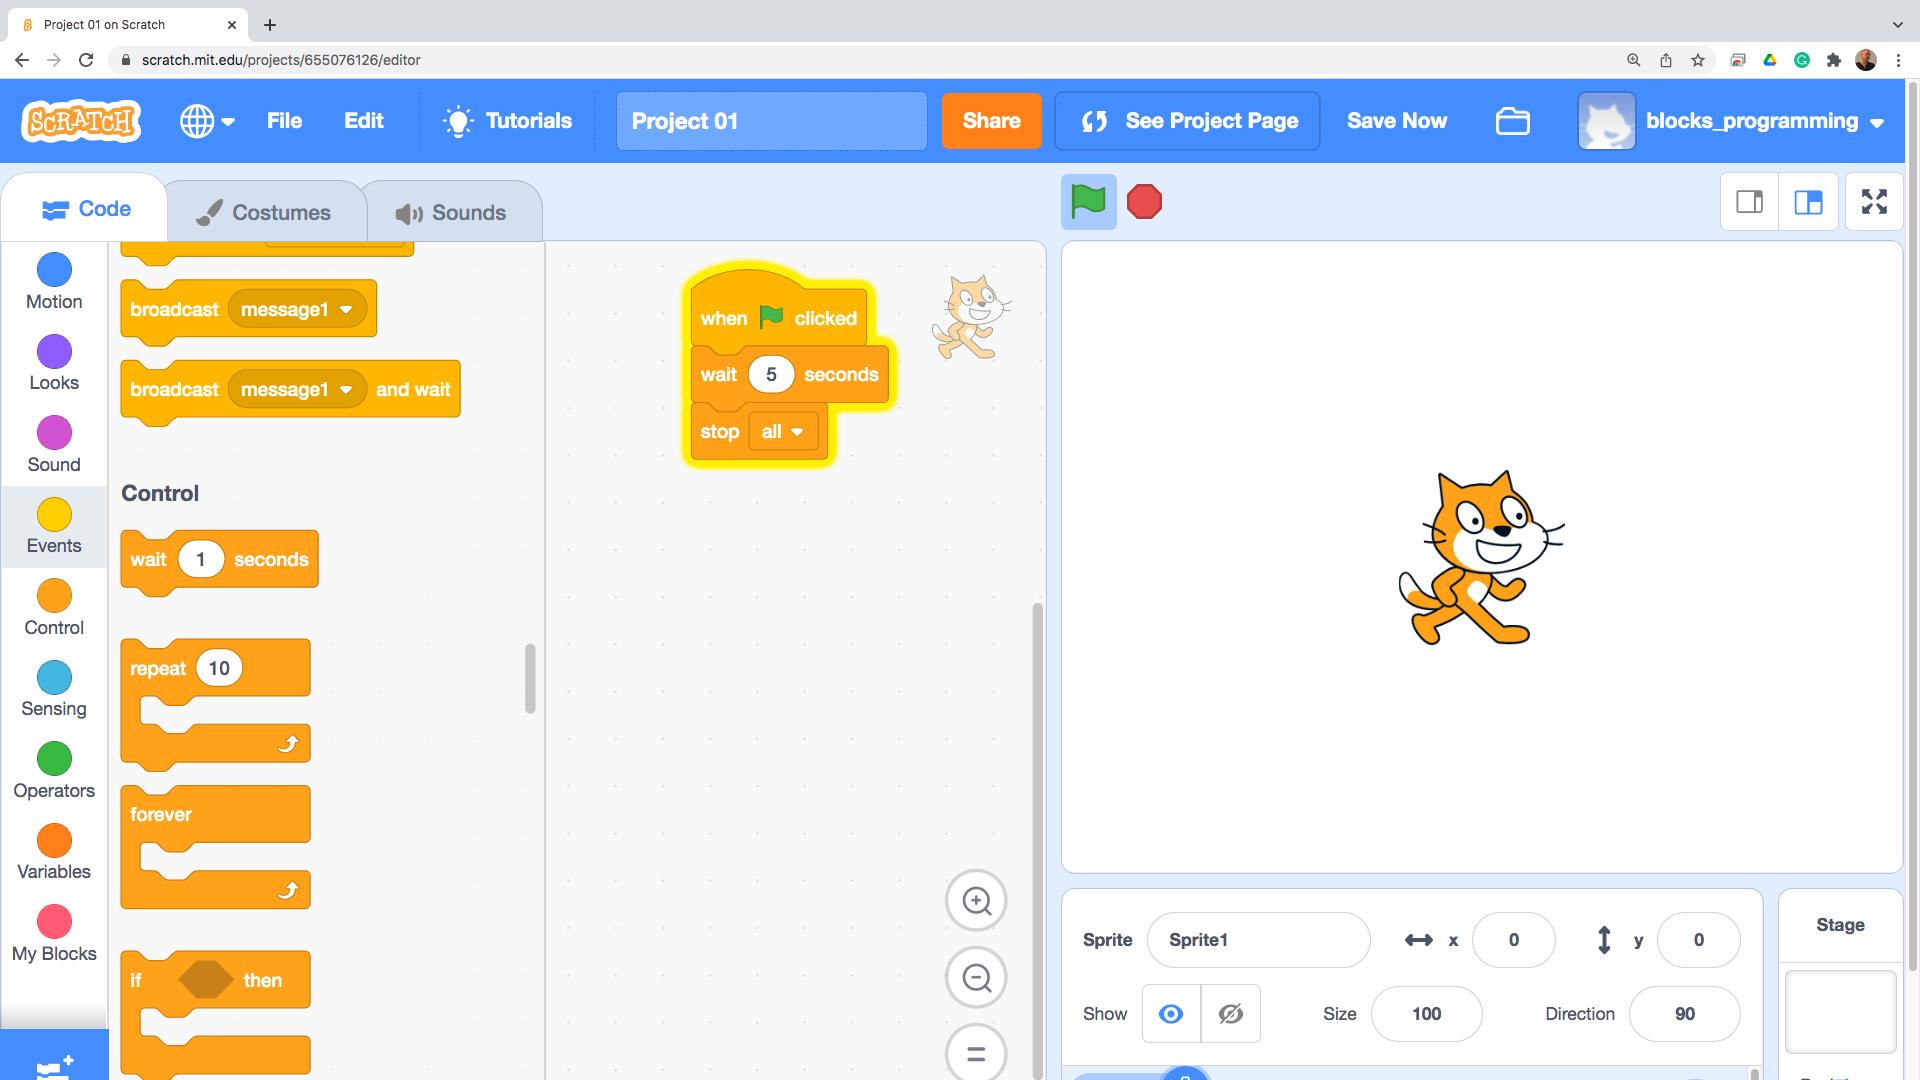
\includegraphics[width=1.0\linewidth,height=0.5\linewidth]{fig020017.png}
   \caption{Wait instruction}
\label{fig020017}
\end{figure}

The purple blocks in Scratch are dedicated to controlling the appearance and speech of the animated character. The first two blocks in this group are specifically designed for displaying lines of text, similar to how text appears in a comic book speech bubble (Fig. \ref{fig020018}).

The first block sets the text displayed on the screen and remains visible until the next instruction is executed. To ensure that the text remains visible to the user for a specific duration, it is essential to include a "wait" block immediately after the text block. This pause allows the text to stay on the screen for the desired amount of time, providing the user with sufficient opportunity to read it.

The second block in the purple group also includes a parameter to determine the duration for which the text will be visible. By specifying the desired period, you can control how long the text remains on the screen before it disappears. This is particularly useful when you want to create a dialogue or add textual information to your project that is displayed for a specific period.

By using these blocks, you can enhance your program's interactive and storytelling aspects, enabling the animated character to communicate with the user through visual text elements.

\begin{figure}[H]
   \centering
   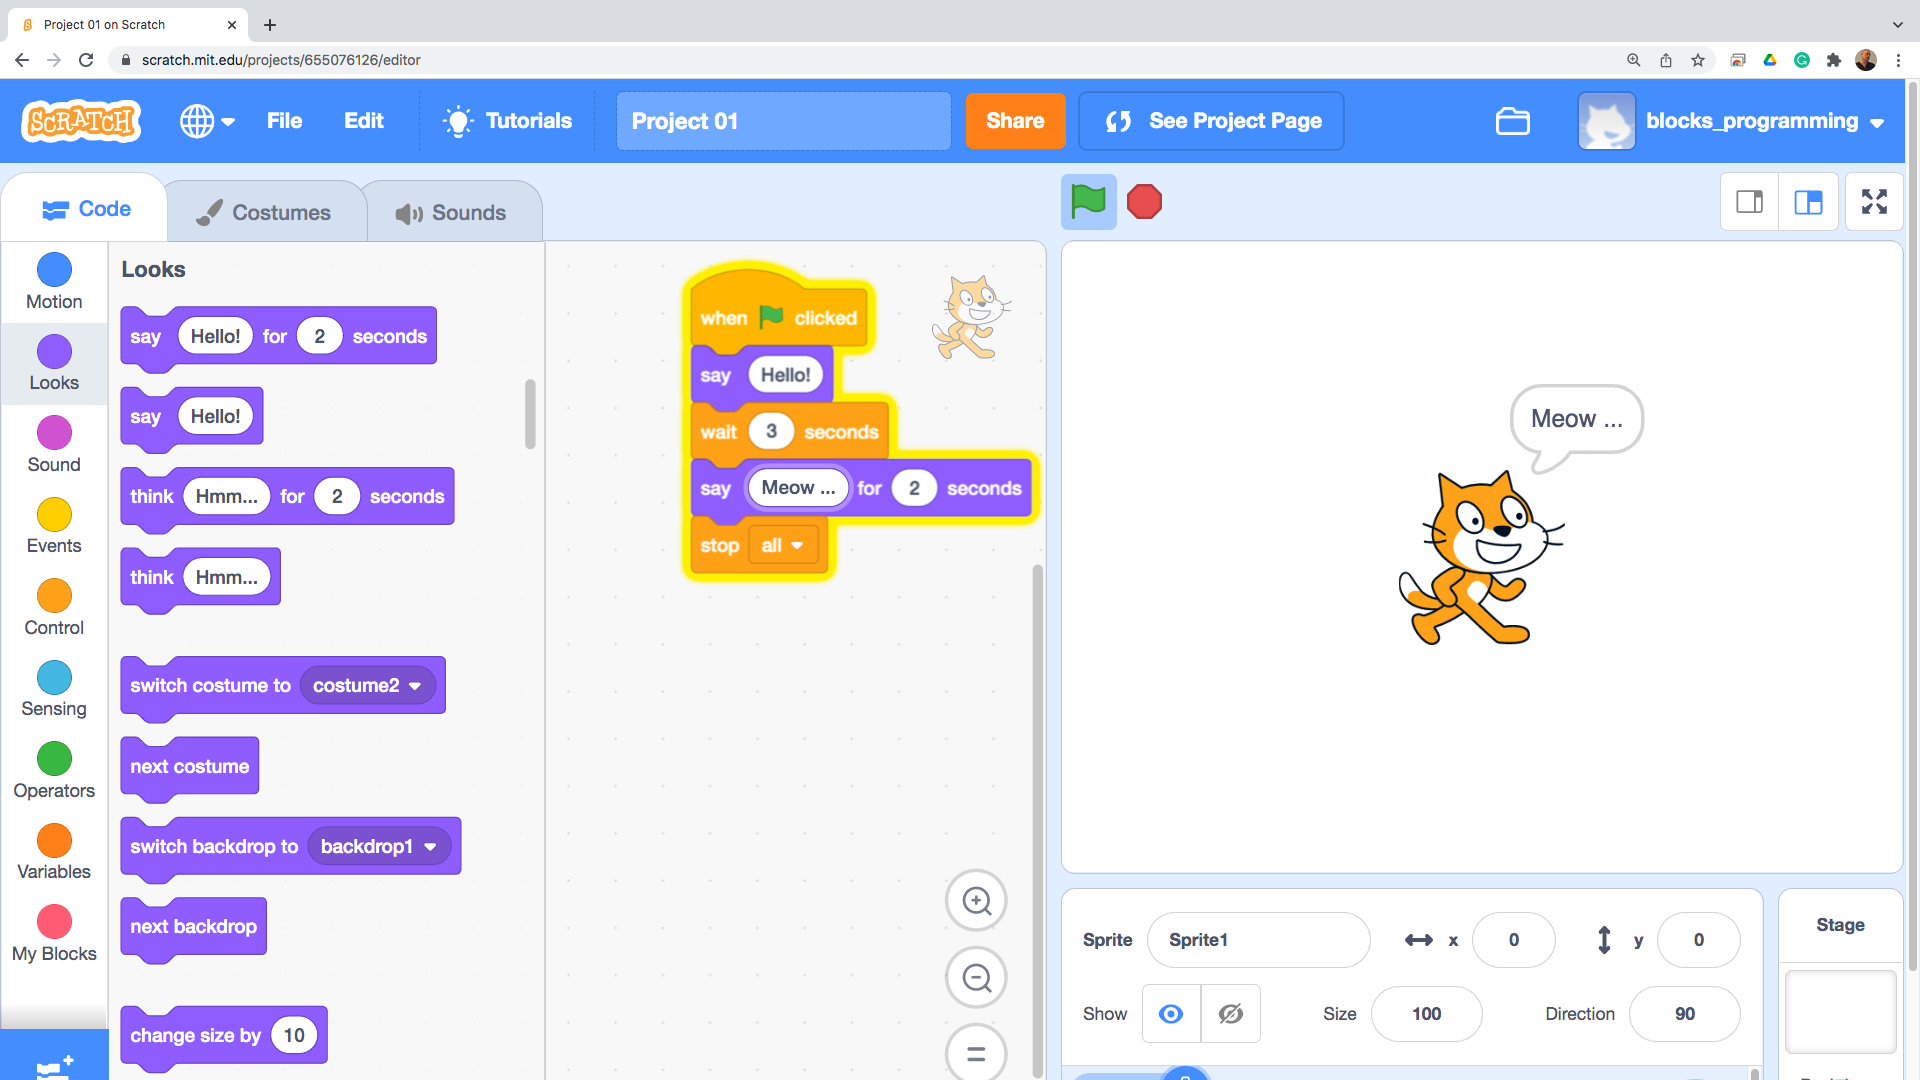
\includegraphics[width=1.0\linewidth,height=0.5\linewidth]{fig020018.png}
   \caption{Writing cues to speak}
\label{fig020018}
\end{figure}

The following two blocks in the purple group serve a similar purpose but with a slight difference. These blocks are designed to display thoughts of the animated character, as opposed to spoken lines (Fig. \ref{fig020019}).

The third block sets the text that represents the character's thoughts. Unlike the previous blocks for spoken lines, the text displayed using this block is typically shown in a different visual style, such as a thought bubble or cloud, to indicate that it represents the character's internal thoughts rather than spoken words.

Similarly to the first block, including a "wait" block after the thought blocks is essential to control how long the thought remains visible on the screen. This ensures that the user has sufficient time to read and comprehend the character's thoughts before disappearing.

These blocks provide a means to add depth and expressiveness to the animated character, allowing them to communicate through spoken dialogue and inner thoughts. By using these blocks effectively, you can create more engaging and immersive storytelling experiences in your Scratch projects.

\begin{figure}[H]
   \centering
   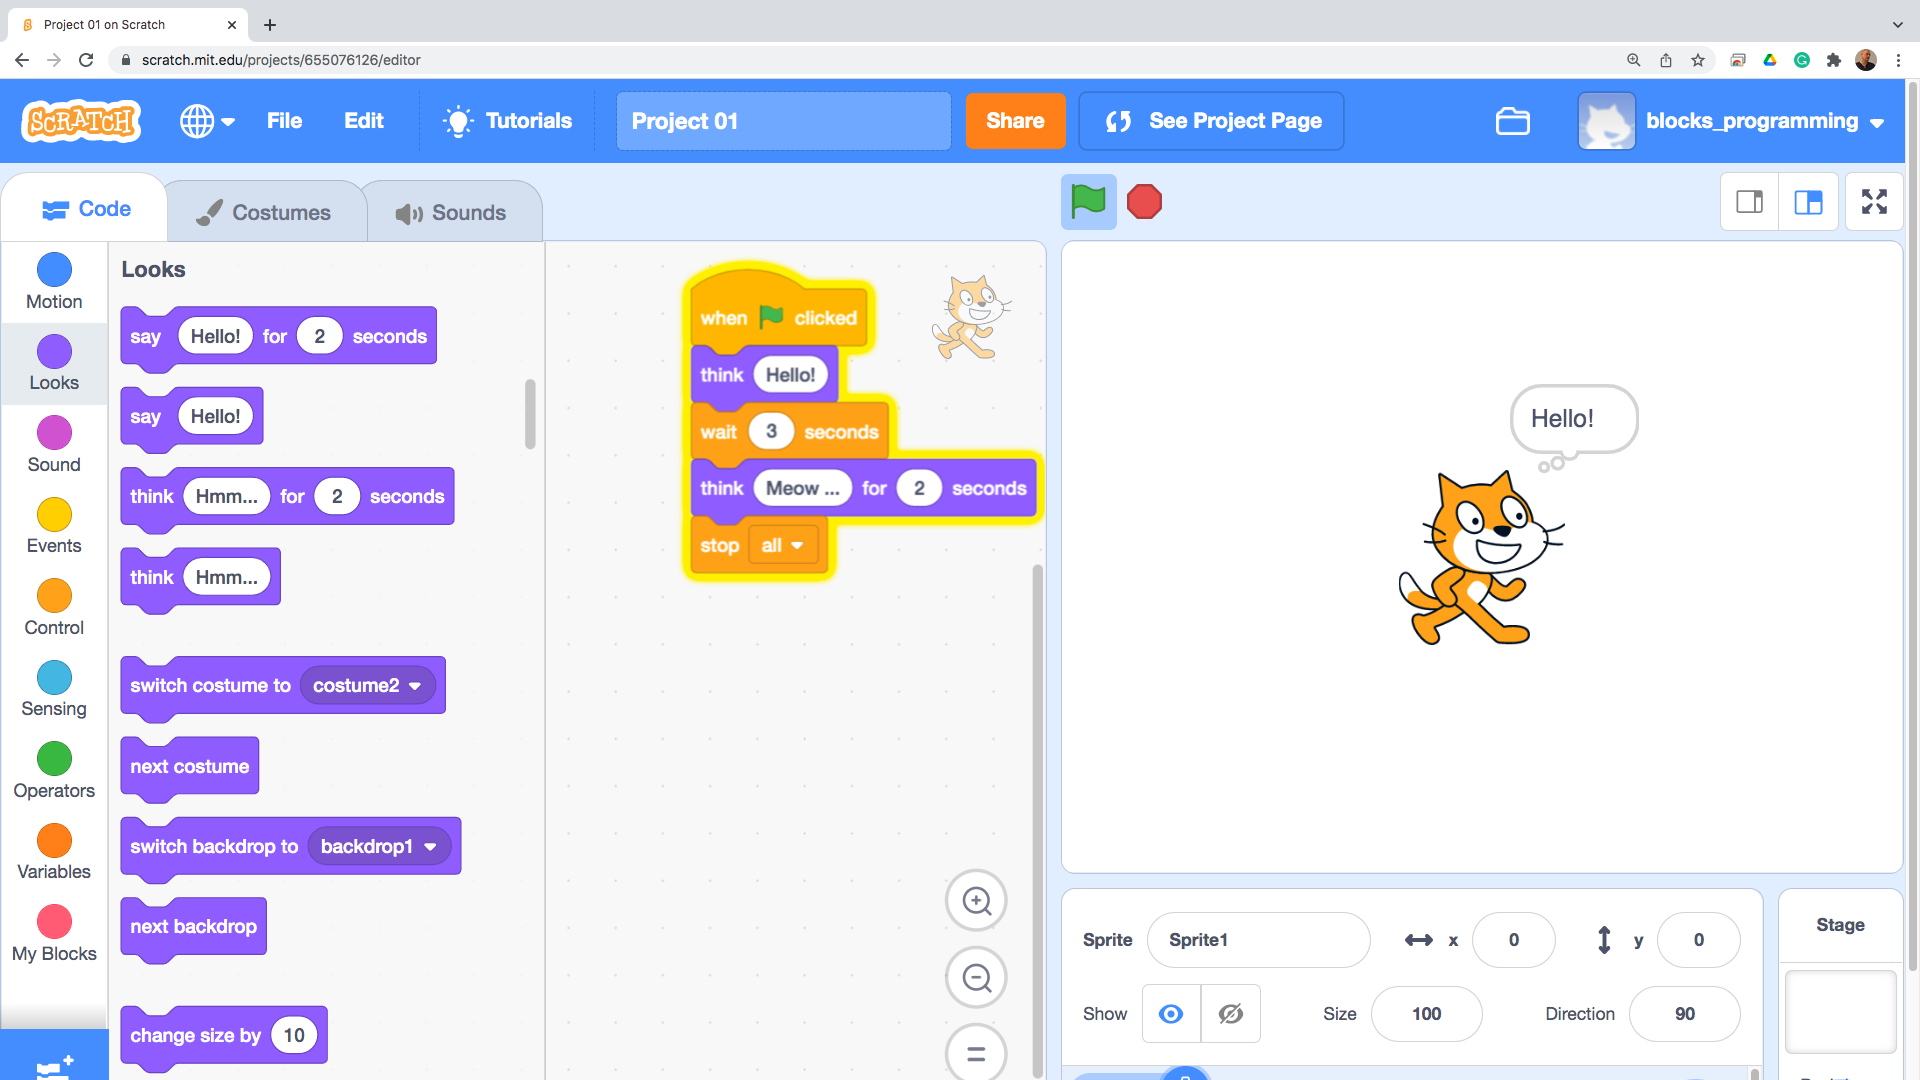
\includegraphics[width=1.0\linewidth,height=0.5\linewidth]{fig020019.png}
   \caption{Writing lines, as a thought}
\label{fig020019}
\end{figure}

In Scratch, animated characters are represented as sprites composed of multiple images or frames depicting the character in different poses or states. To create the illusion of movement or animation, we can use two specific blocks (Fig. \ref{fig020020}) to control the frames displayed by the sprite.

The first block allows us to set a specific frame within the sprite. By specifying the frame number, we can choose a particular pose or image for the character. This block is useful for displaying a specific frame without transitioning to the next one.

The second block, on the other hand, advances the sprite to the next frame in the sequence. This creates a smooth transition between frames and gives the impression of motion. By repeatedly using this block, we can create an animation by cycling through the frames of the sprite.

Combining these two blocks and controlling the timing and sequence of frame changes, we can bring our animated characters to life, making them move, perform actions, and express emotions in our Scratch projects.

\begin{figure}[H]
   \centering
   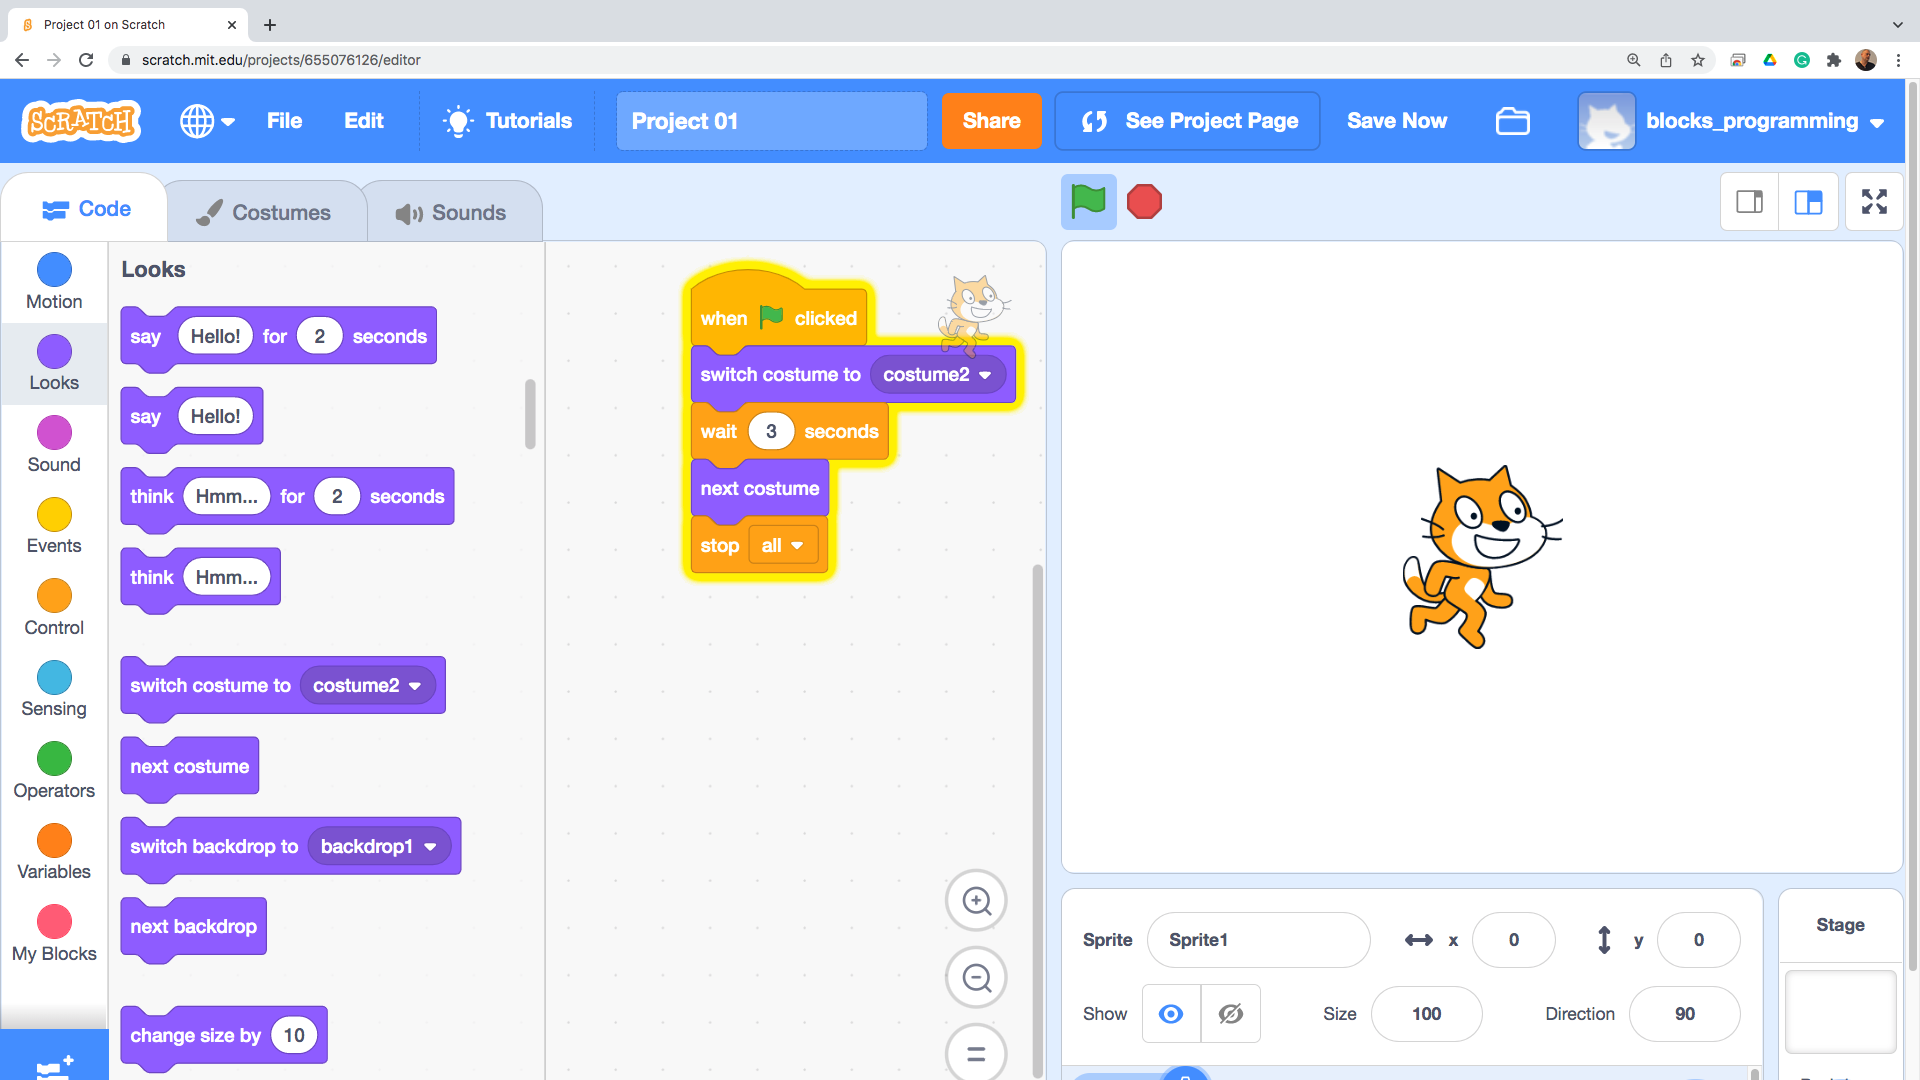
\includegraphics[width=1.0\linewidth,height=0.5\linewidth]{fig020020.png}
   \caption{Changing Poses}
\label{fig020020}
\end{figure}

In Scratch, along with the animated characters represented as sprites, we also can change the background image of the stage or work scene. This allows us to create dynamic and visually engaging projects. To control the background image, Scratch provides two distinct blocks (Fig. \ref{fig020021}).

The first block enables us to select background images in various ways. We can choose the next image in the sequence, return to the previous image, select a random image, or even specify a specific image by its name. This gives us flexibility in determining how the background changes throughout the program.

The second block sets the next image in the sequence as the background. Using this block repeatedly, we can create smooth transitions between different background images, creating a visually appealing and dynamic backdrop for our projects.

With these blocks, we can transform the environment in which our sprites interact, setting the mood, location, or context of our Scratch programs. By carefully selecting and arranging background images, we can enhance the storytelling and immersion of our projects.

\begin{figure}[H]
   \centering
   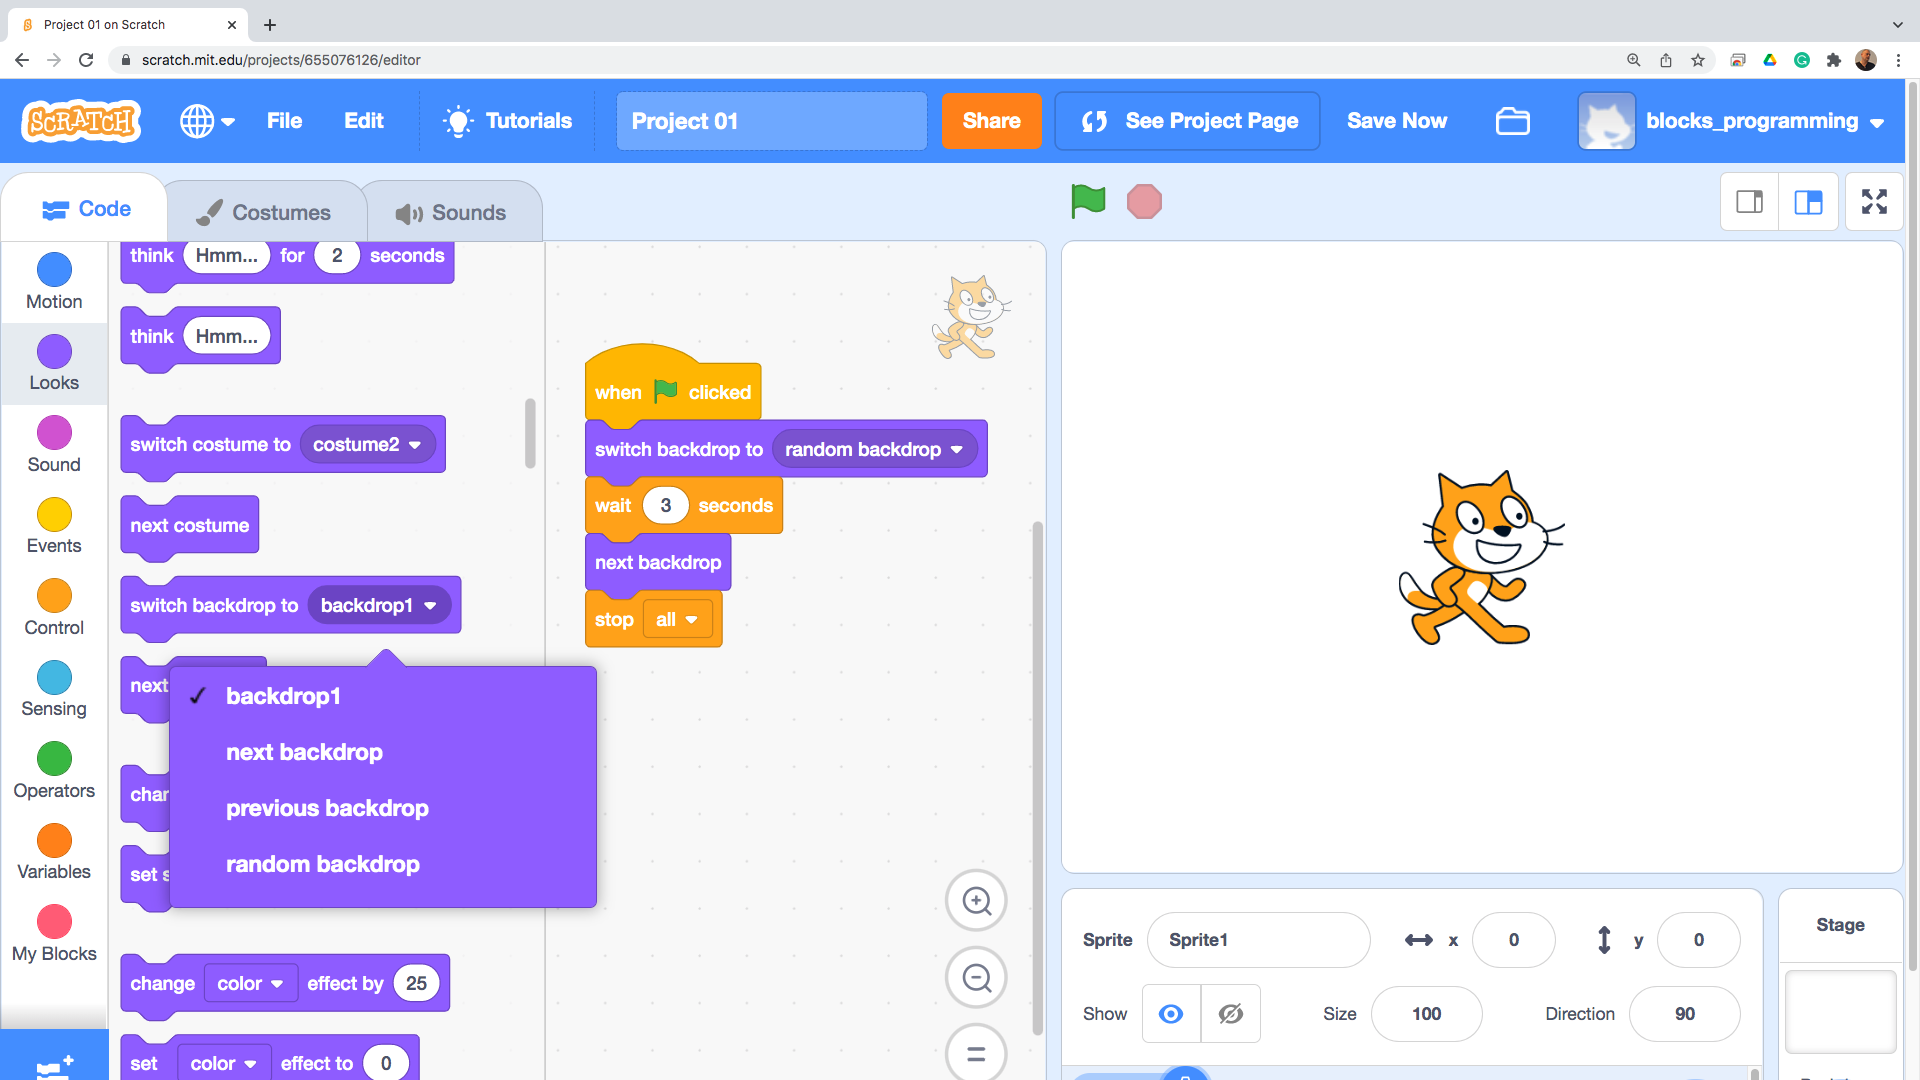
\includegraphics[width=1.0\linewidth,height=0.5\linewidth]{fig020021.png}
   \caption{Change background}
\label{fig020021}
\end{figure}

In Scratch, two blocks are dedicated to resizing the animated characters or sprites. These blocks allow us to adjust the sprites' size according to our specific requirements (Fig. \ref{fig020022}).

The first block allows us to resize the sprite using absolute values. We can specify the desired width and height of the sprite in pixels, providing precise control over its dimensions. This block is useful when resizing the sprite to specific pixel dimensions for alignment or design purposes.

The second block enables us to resize the sprite using percentages relative to its original size. We can specify the percentage we want to scale up or down the sprite. This block is handy when we proportionally adjust the sprite's size based on a relative scale.

Using these blocks, we can dynamically modify the size of our animated characters to create visual effects, emphasize specific actions, or fit them into different contexts within our projects. The ability to resize the sprites gives us flexibility and control over their appearance, allowing us to bring our creative ideas to life in Scratch.

\begin{figure}[H]
   \centering
   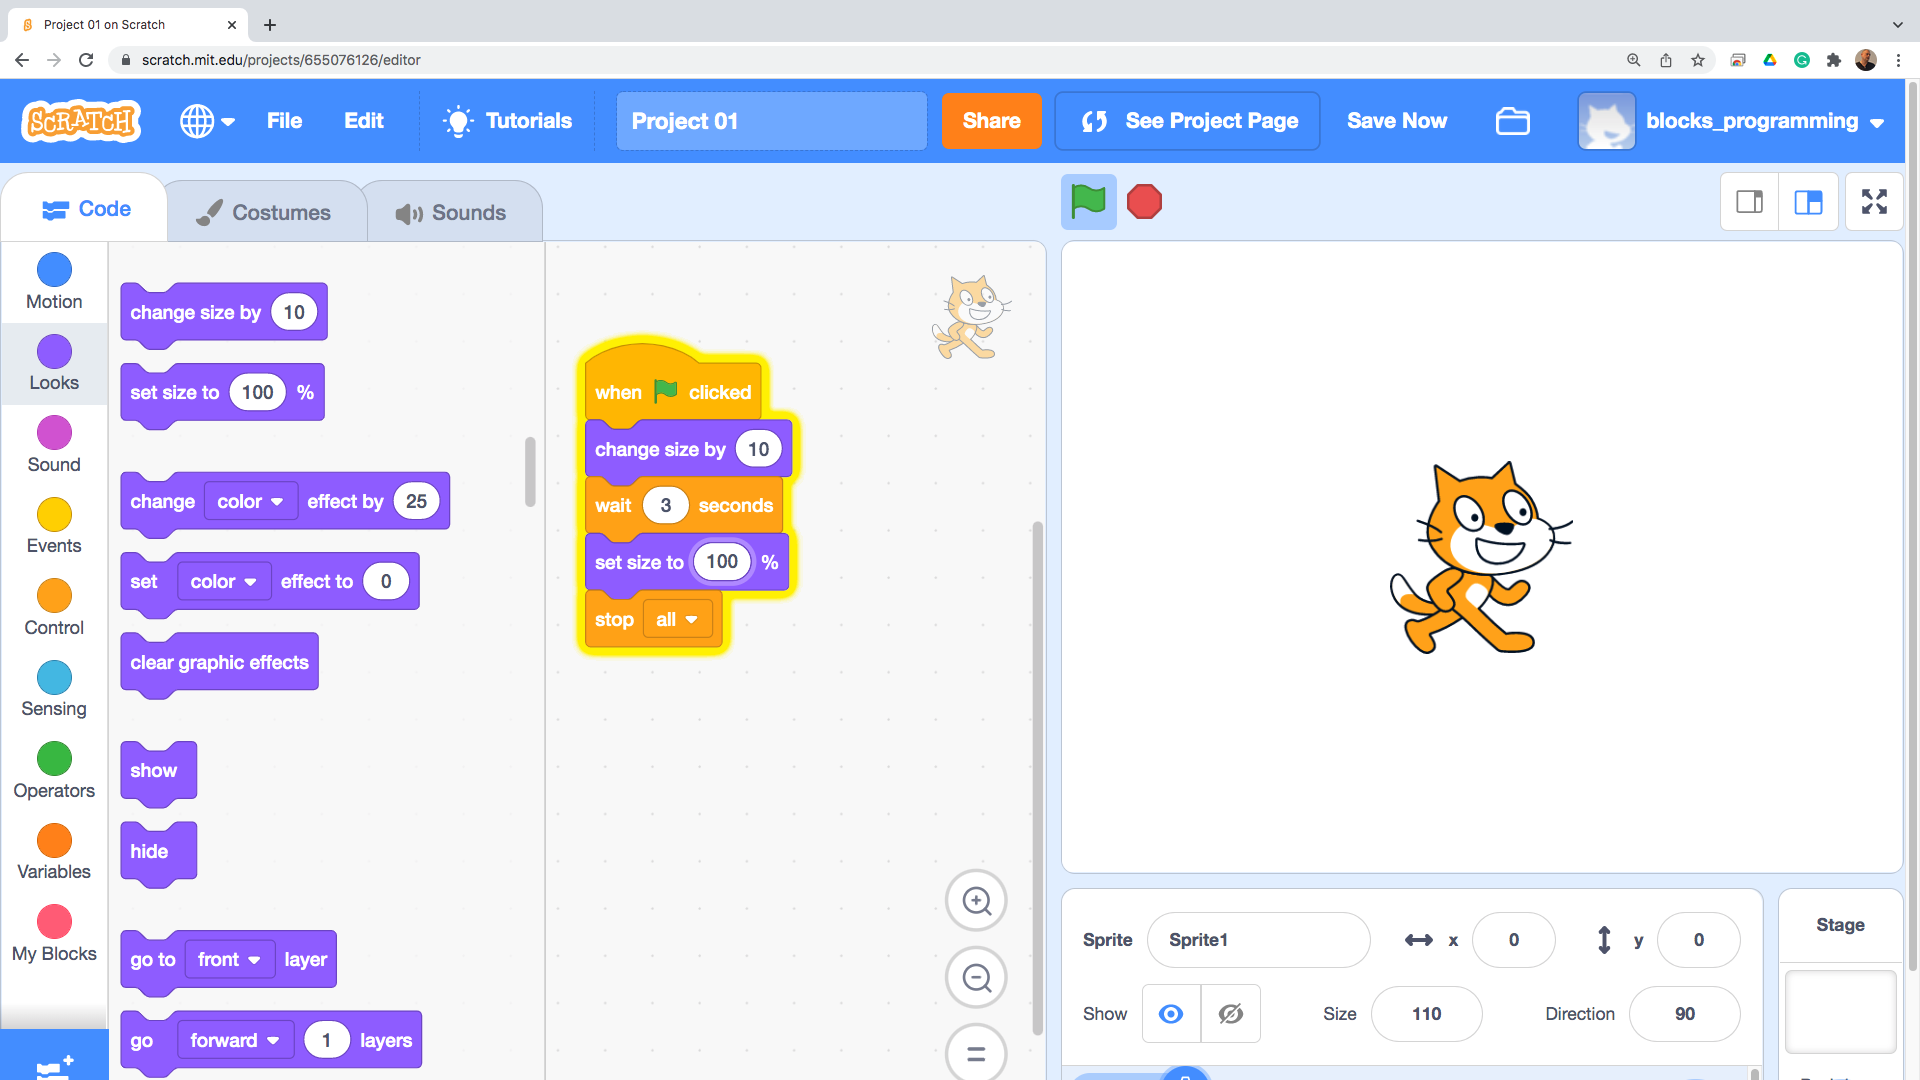
\includegraphics[width=1.0\linewidth,height=0.5\linewidth]{fig020022.png}
   \caption{Resize}
\label{fig020022}
\end{figure}

Within Scratch, we have three blocks that allow us to modify the visual appearance of the animated characters or sprites (Fig. \ref{fig020023}). These blocks will enable us to apply various visual effects, distortions, and adjustments to enhance the visual layout of our characters.

The first two blocks enable us to introduce changes to the character's appearance. We can apply modifications such as changing colors, adding distortions, pixelation, mosaic effects, adjusting transparency, or altering brightness. These changes can be either relative to the character's current state or set as an absolute change.

It is important to note that when applying these visual effects, giving a few seconds of delay allows the user to discern the changes. By providing this pause, we ensure the modifications are visibly apparent before the program progresses.

The third block available in this group allows us to cancel any applied modifications and restore the character to its original state. This block is useful when we want to reset or remove any visual alterations made to the character.

With these blocks, we can unleash our creativity and add captivating visual transformations to our animated characters. By incorporating changes in color, distortion effects, and other visual adjustments, we can bring life and uniqueness to our characters, making them visually appealing and engaging to the users.

\begin{figure}[H]
   \centering
   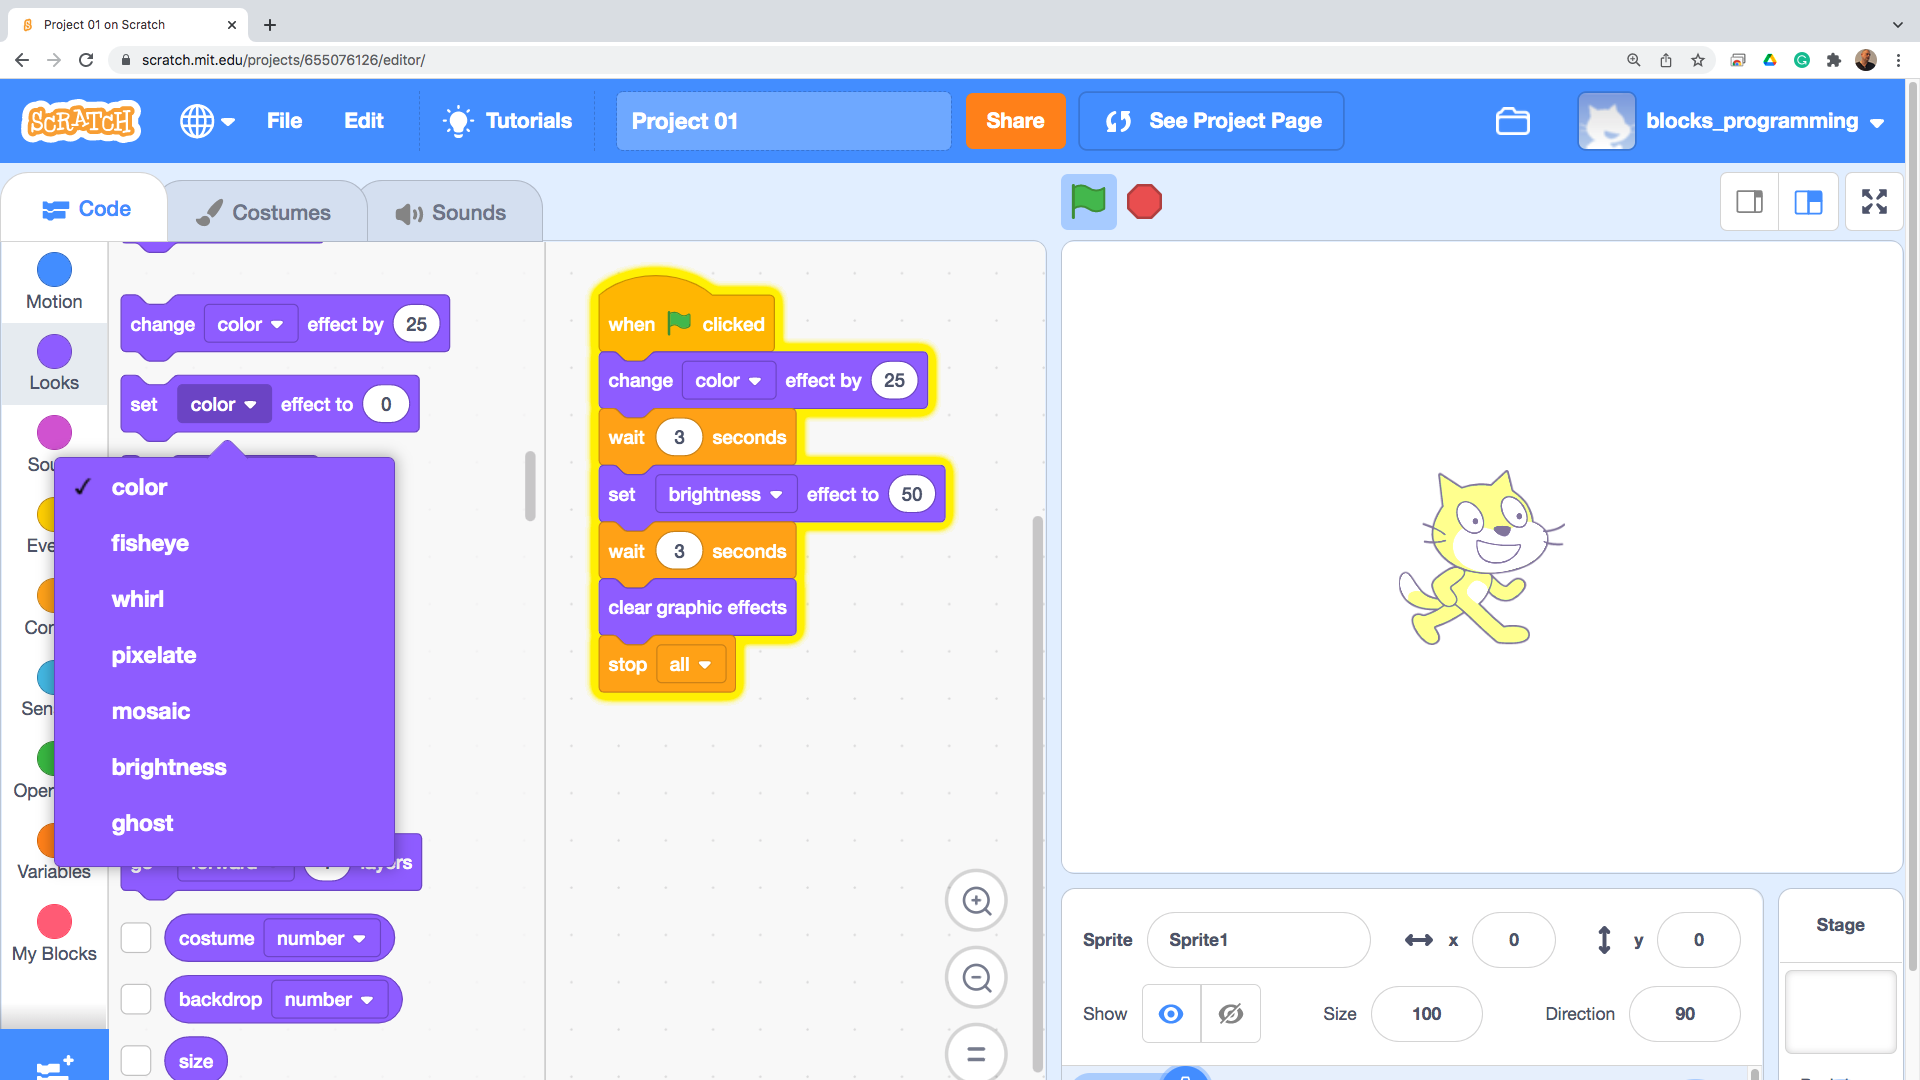
\includegraphics[width=1.0\linewidth,height=0.5\linewidth]{fig020023.png}
   \caption{Change appearance}
\label{fig020023}
\end{figure}

Working with sprites in Scratch primarily allows us to create stunning animated effects. Within a scene, different animated characters, or sprites, can interact with each other, creating dynamic and engaging experiences. The script or program developed for the project determines when each character appears on the scene and when they disappear.

To control the appearance and disappearance of sprites, Scratch provides two specific blocks designed for these actions (Fig. \ref{fig020024}). These blocks allow us to control the visibility of sprites at different moments during the program's execution.

The first block is used to make a sprite appear on the scene. Using this block, we can specify when a sprite should become visible to the user. This can be synchronized with other events or conditions in the program to create desired effects.

Conversely, the second block is used to make a sprite disappear from the scene. With this block, we can define when a sprite should no longer be visible, creating smooth transitions or removing sprites from the scene when their role or purpose is fulfilled.

Using these appearance and disappearance blocks gives us precise control over when sprites enter and exit the stage, allowing us to orchestrate complex animations, character interactions, and storytelling within our Scratch projects.

\begin{figure}[H]
   \centering
   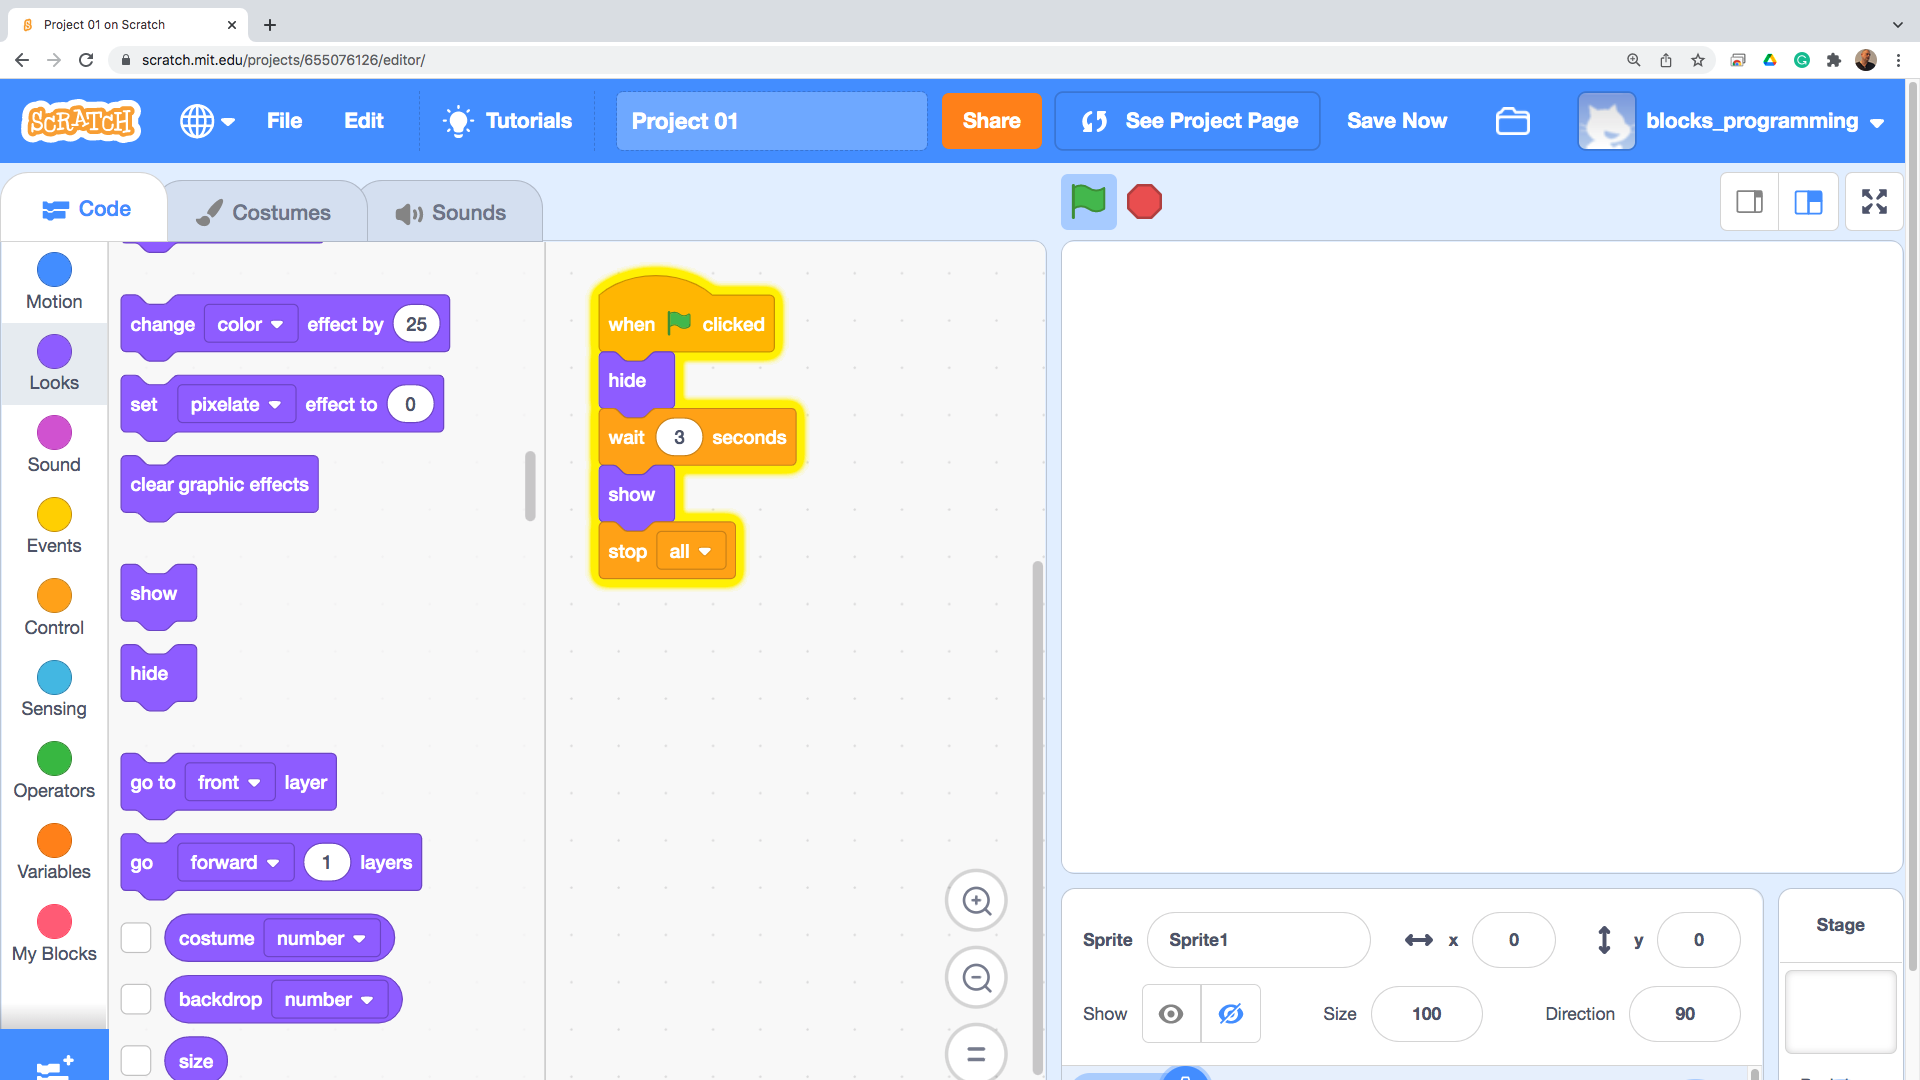
\includegraphics[width=1.0\linewidth,height=0.5\linewidth]{fig020024.png}
   \caption{Hide and show}
\label{fig020024}
\end{figure}

Many bitmap software products, such as Adobe Photoshop, GIMP, Microsoft Word, LibreOffice Draw, and others, utilize a layered approach to organize different images. This layering system is logical and essential for managing complex compositions where sprites or elements may overlap at specific points in time. In some graphics software, the concept of layers is akin to a Z-buffer, which determines elements' depth or stacking order.

In Scratch, working with layers is also available, providing control over the visibility and positioning of sprites within the scene. Scratch offers two specific blocks that allow sprites to move forward and backward through the layers, adjusting their stacking order and determining which sprites appear in front or behind others (Fig. \ref{fig020025}).

The "go to front layer" block brings a sprite to the front, ensuring it is positioned above other sprites in the layer stack. This can be useful when you want a particular sprite to be in the foreground or to appear above all other elements.

Conversely, the "go back [number] layers" block moves a sprite back in the stack, positioning it behind other sprites. By specifying the number of layers to move back, you can precisely control the sprite's placement in relation to other elements in the scene.

These layering blocks in Scratch provide flexibility and control over the visual arrangement of sprites, enabling the creation of intricate compositions and interactions within your projects.

\begin{figure}[H]
   \centering
   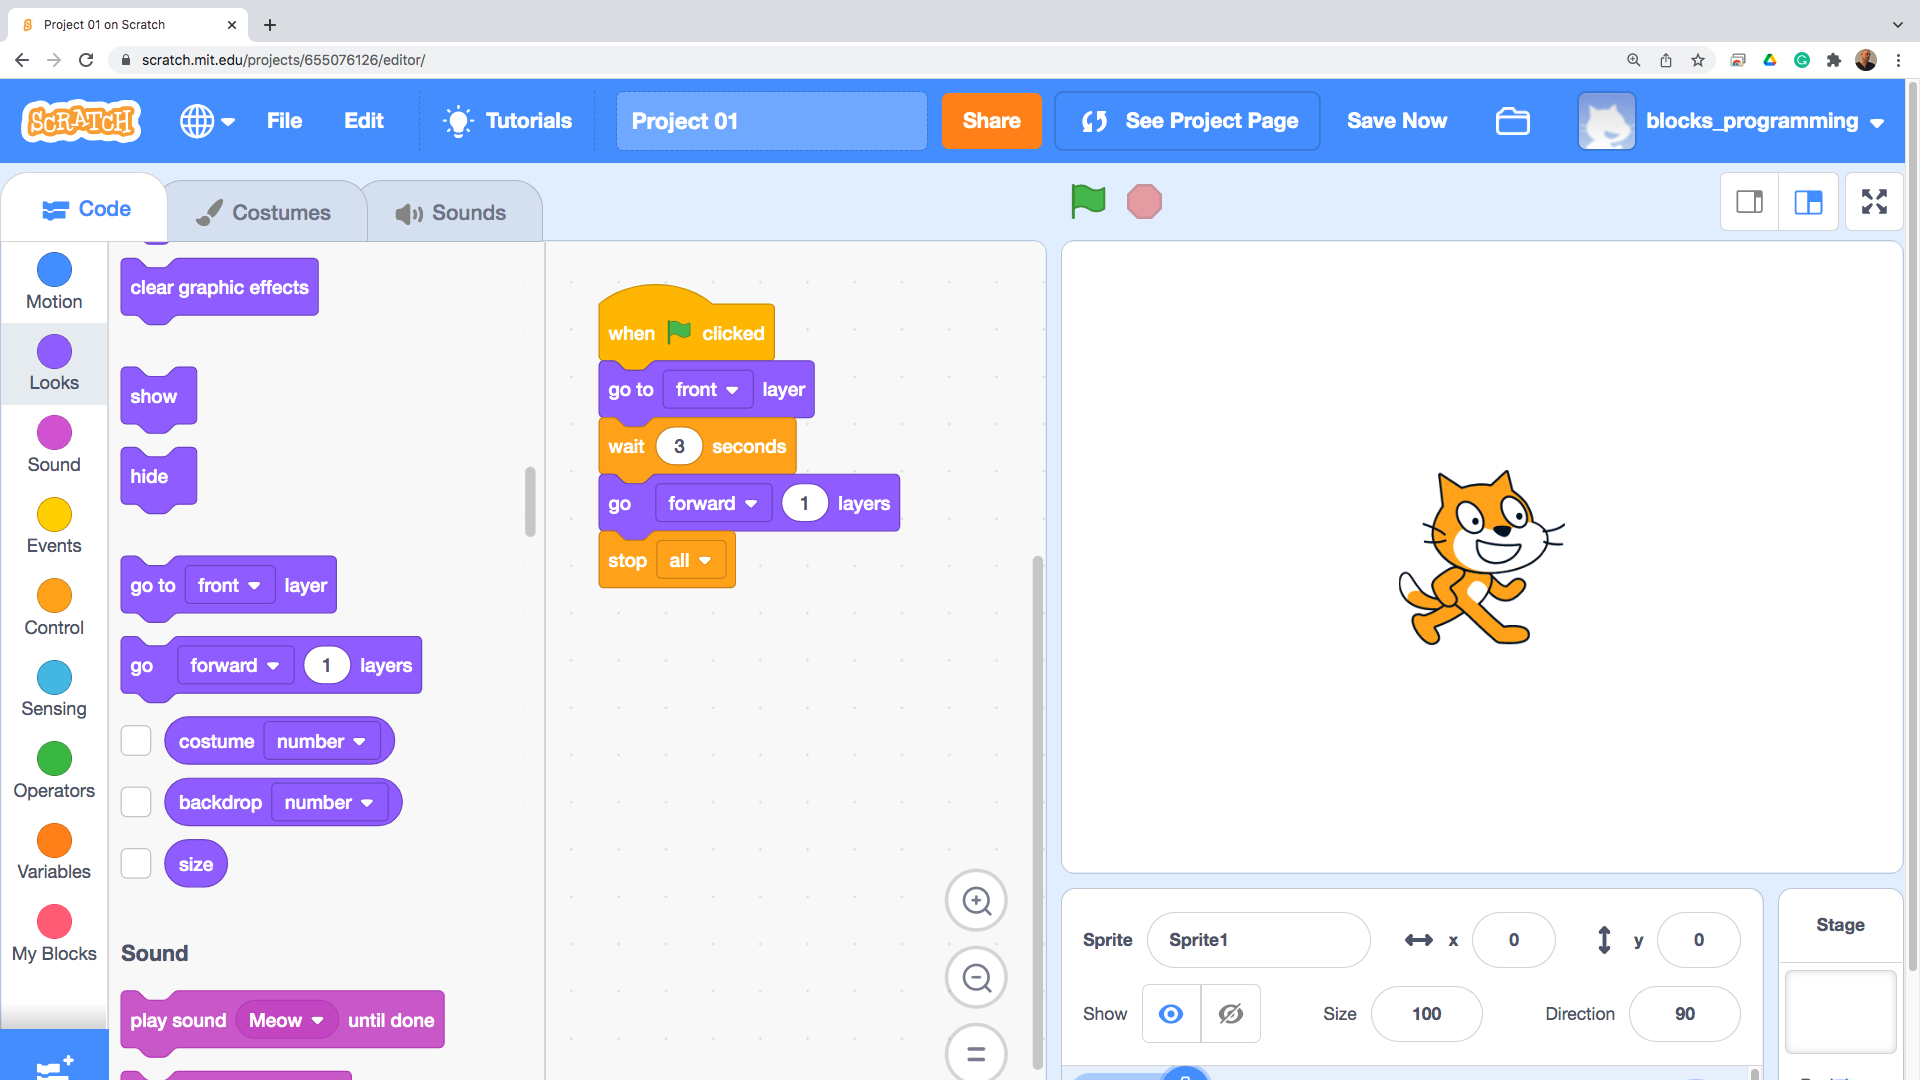
\includegraphics[width=1.0\linewidth,height=0.5\linewidth]{fig020025.png}
   \caption{Navigation through layers}
\label{fig020025}
\end{figure}

Scratch's magenta group of blocks is dedicated to sound control and manipulation. These blocks enable the integration of audio elements into your projects. Three key blocks in this group (Fig. \ref{fig020026}) facilitate sound management.

The first block, "play sound", allows you to play a specific sound file. When this block is executed, the sound will play in its entirety before moving on to the next block in the sequence. This is useful to ensure that a sound is played entirely before triggering other actions or events.

The second block, "start sound until done", starts playing a sound and waits until it is finished before proceeding to the next block. This block is helpful for synchronizing actions or animations with the duration of a sound.

The third block, "stop all sounds", is used to stop all playing sounds. When executed, it immediately halts any ongoing sound playback in the project.

Additionally, Scratch allows recording sounds directly from the user's computer, expanding the range of audio content that can be incorporated into projects. This feature allows for customization and personalization, enabling users to utilize their own recorded sounds.

By utilizing the sound blocks in Scratch, you can enhance your projects with audio effects, background music, sound effects, and interactive sound elements, creating a more engaging and immersive experience for users.

\begin{figure}[H]
   \centering
   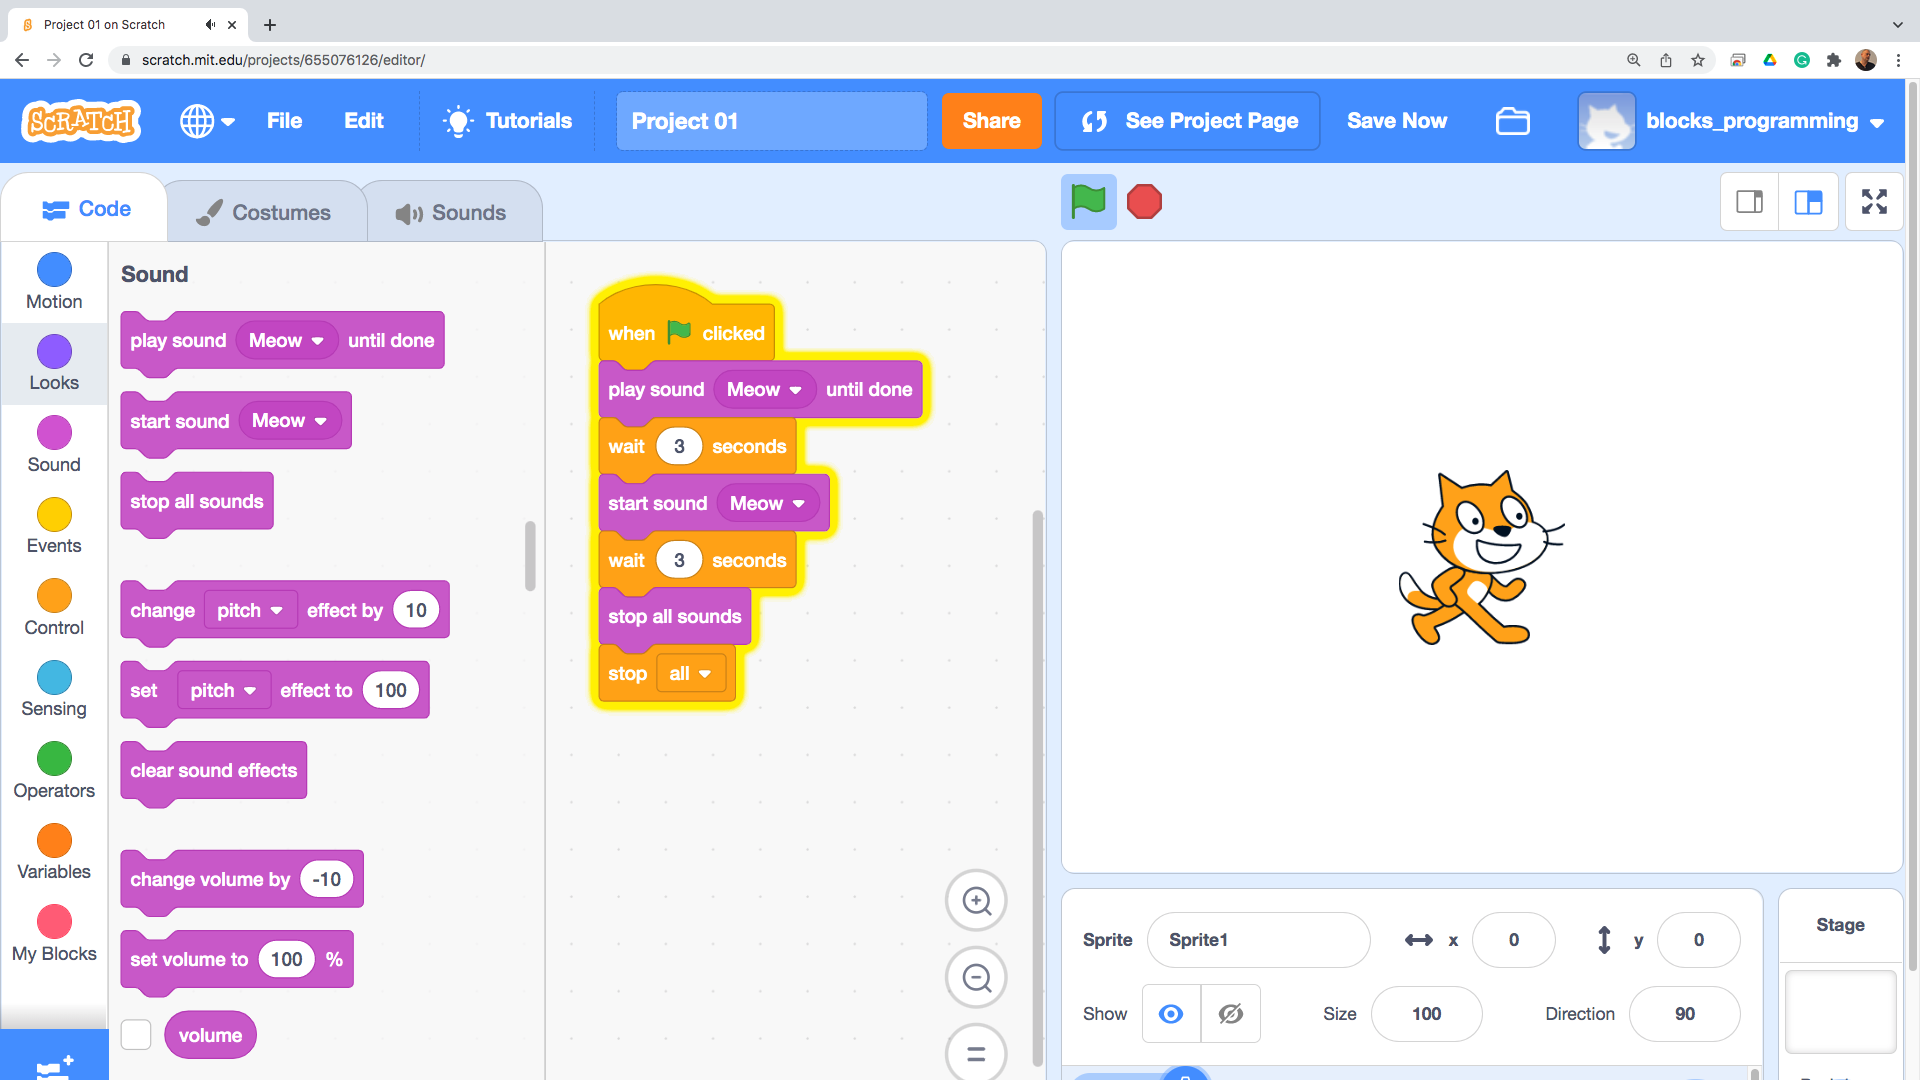
\includegraphics[width=1.0\linewidth,height=0.5\linewidth]{fig020026.png}
   \caption{Playing Sounds}
\label{fig020026}
\end{figure}

In Scratch, you can modify the characteristics of sounds using the "pitch" and "stereo" blocks. These blocks allow you to manipulate the pitch (frequency) and stereo positioning (left/right balance) of the sound, respectively (Fig. \ref{fig020027}).

The "pitch" block allows you to adjust the frequency of a sound, which affects its perceived pitch. By specifying a numerical value, you can increase or decrease the pitch of the sound, creating higher or lower tones. This can be useful for creating melodic variations, altering the mood of a sound effect, or experimenting with different musical effects.

The "stereo" block enables you to control the stereo positioning of a sound in the virtual soundscape. By assigning a numerical value, you can adjust the balance between the left and right channels of the sound. This manipulation affects the perceived location of the sound source in the stereo field, allowing you to create immersive and spatial audio experiences.

By combining these blocks with other programming elements in Scratch, such as conditional statements or user interactions, you can dynamically modify sounds' pitch and stereo characteristics in response to specific events or conditions. This adds an extra dimension of control and creativity to your sound design and allows for more expressive and engaging projects.

\begin{figure}[H]
   \centering
   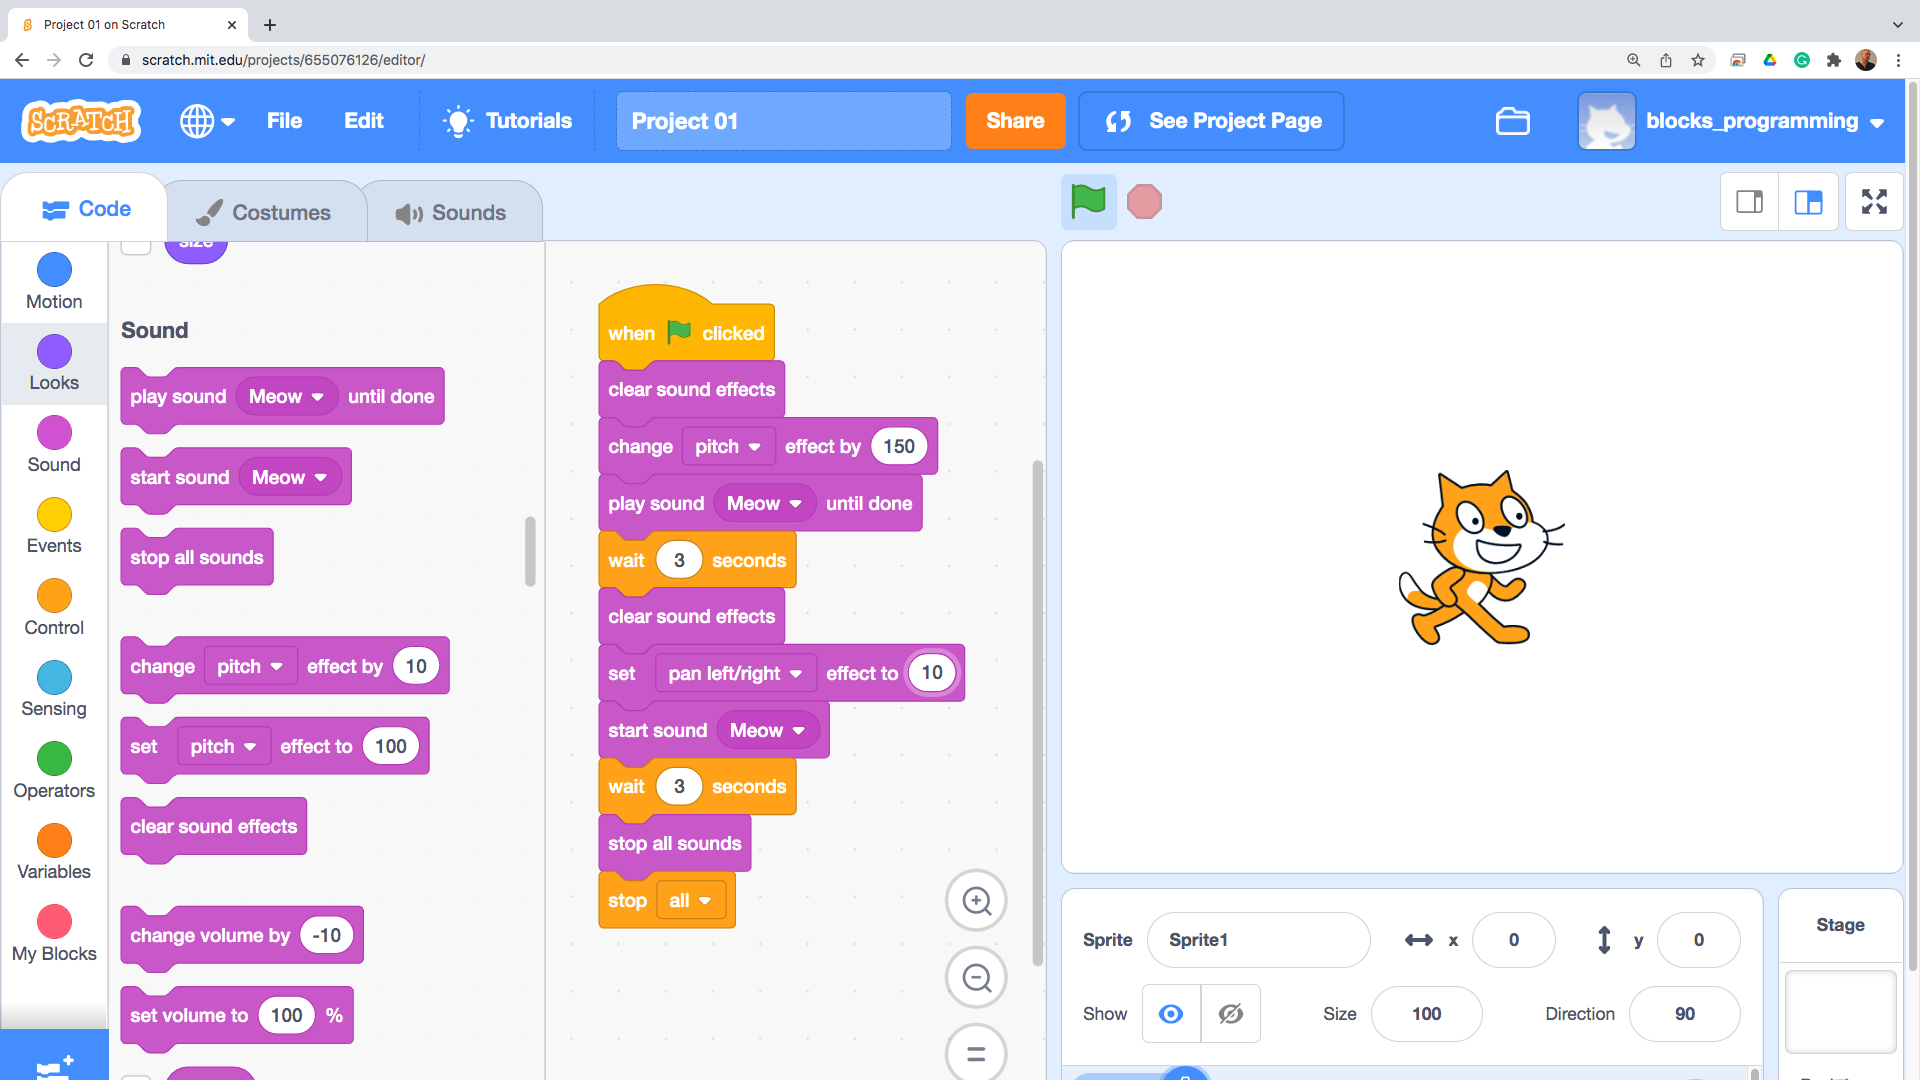
\includegraphics[width=1.0\linewidth,height=0.5\linewidth]{fig020027.png}
   \caption{Sound Characteristics}
\label{fig020027}
\end{figure}

In Scratch, you can control the strength or volume of sounds using two blocks (Fig. \ref{fig020028}). These blocks allow you to adjust the volume of the sound, providing greater control over the audio experience.

The first block allows you to set the volume of the sound in absolute terms. By specifying a numerical value, you can directly control the loudness of the sound, with higher values producing louder sounds and lower values resulting in quieter sounds. This block is useful when you want precise control over the volume level of a specific sound.

The second block enables you to adjust the volume of the sound as a percentage relative to its original strength. By specifying a numerical value between 0 and 100, you can increase or decrease the volume of the sound proportionally. This block is handy when you want to adjust the volume of a sound dynamically or in relation to other factors in your project.

Using these volume control blocks combined with other programming elements, such as loops or conditional statements, you can create more immersive sound experiences, fade-in or fade-out effects, or even design interactive soundscapes where the volume responds to user interactions or specific events.

Experimenting with different volume settings and combinations of sounds can enhance the overall audio quality of your projects and create a more engaging and enjoyable experience for your users.

\begin{figure}[H]
   \centering
   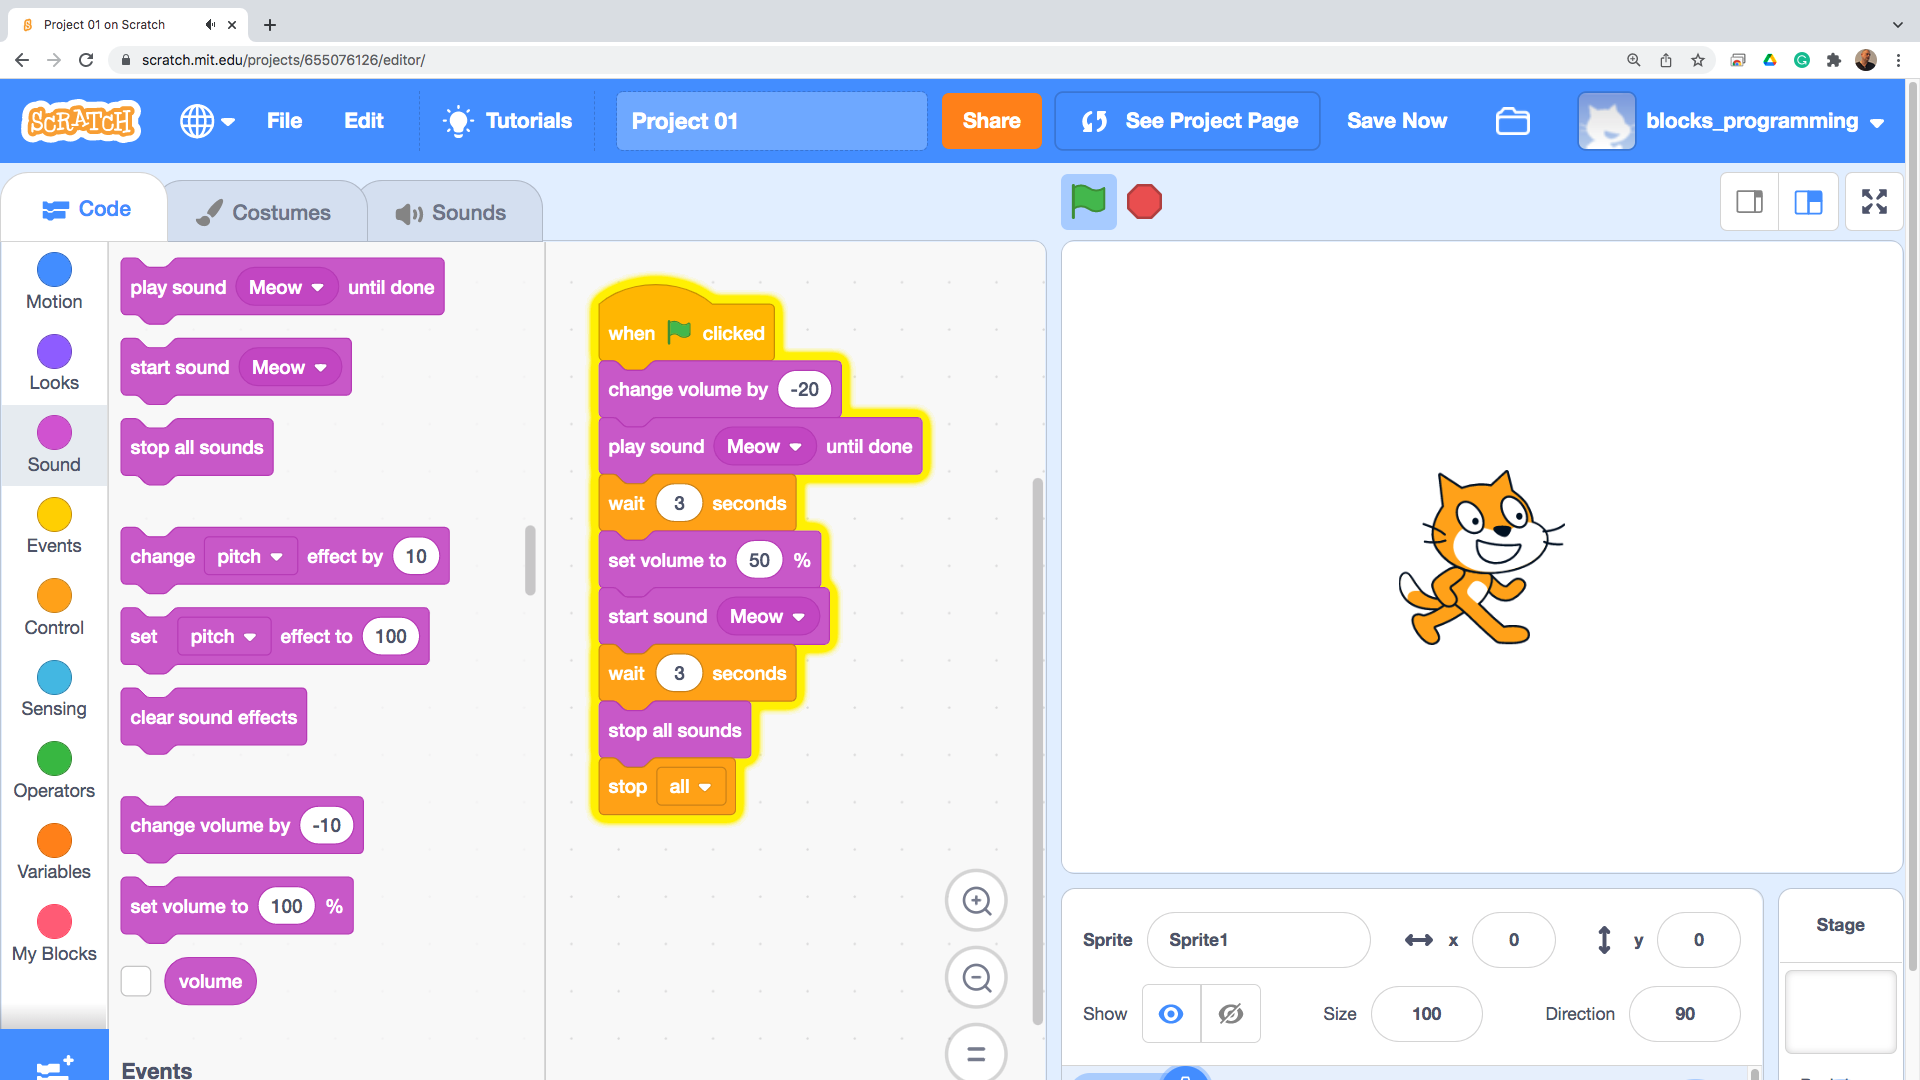
\includegraphics[width=1.0\linewidth,height=0.5\linewidth]{fig020028.png}
   \caption{Volume}
\label{fig020028}
\end{figure}

The orange group of blocks in Scratch is dedicated to handling events. Events provide a way to execute instructions when there is no predetermined point at which program instructions must be performed. One example of an event is when a user presses a button on the keyboard.

Scratch provides specific blocks to respond to keyboard events that allow you to detect when a particular key is pressed. Using these blocks, you can trigger actions or initiate a sequence of instructions in response to user input.

The block shown in Fig. \ref{fig020029} represents a keyboard event block. It allows you to specify a key on the keyboard that should trigger the associated instructions. The instructions connected to the event block will be executed when that key is pressed.

Events provide a powerful way to make your programs interactive and responsive to user actions. By combining event blocks with other programming elements, such as loops, conditions, and control structures, you can create engaging experiences that react to user input in real time.

Remember to consider user experience when designing event-driven programs. Provide clear instructions and feedback to users, and ensure that the events you choose to respond to are intuitive and aligned with the purpose of your project.

With the event blocks in the orange group, you can create dynamic and interactive projects that engage users and make your Scratch creations come to life.

\begin{figure}[H]
   \centering
   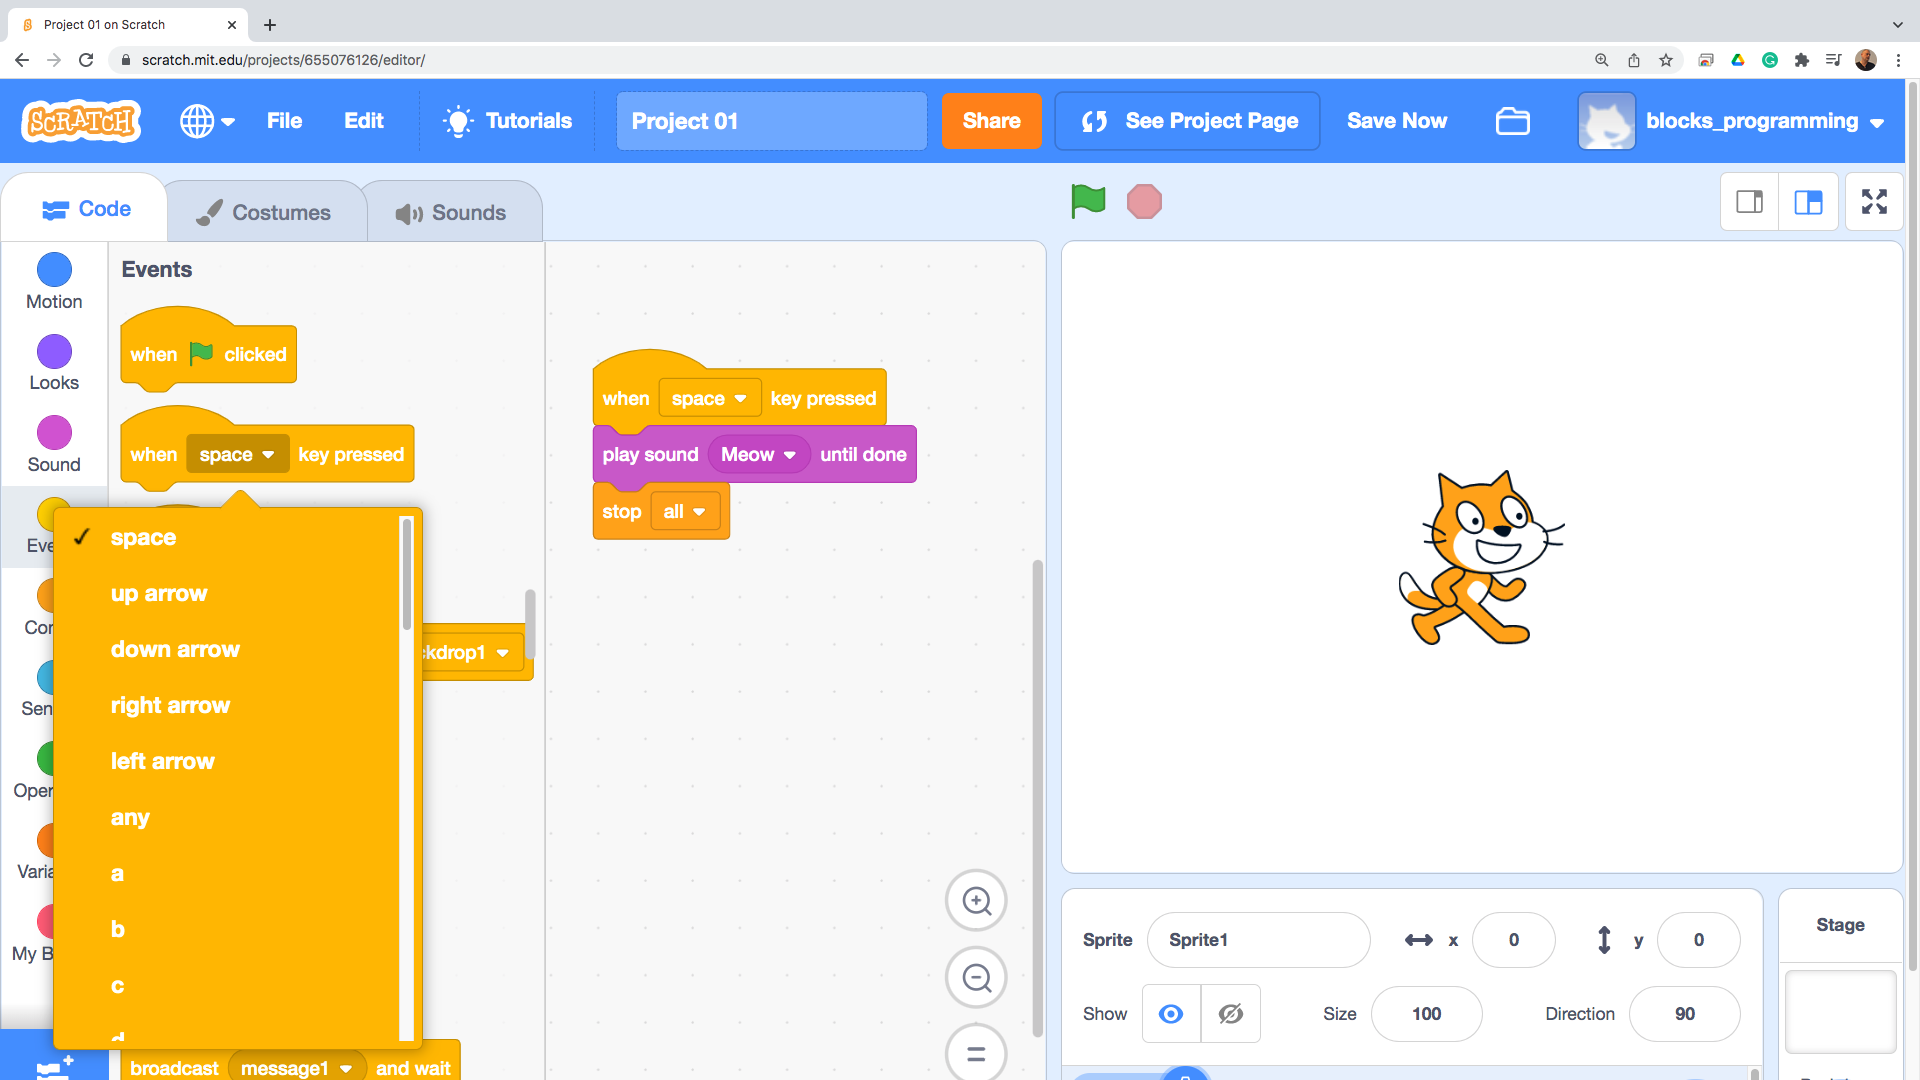
\includegraphics[width=1.0\linewidth,height=0.5\linewidth]{fig020029.png}
   \caption{Key Press Event}
\label{fig020029}
\end{figure}

Mouse clicking on a specific sprite can also be handled in Scratch using a dedicated block (Fig. \ref{fig020030}). This block allows you to define instructions that should be executed when the mouse clicks the sprite.

Attaching this block to a sprite creates an event listener that detects mouse clicks specifically on that sprite. This provides a way to create interactive elements in your project, where users can interact with the sprite by clicking on it.

Connecting other blocks and instructions to the mouse-click event block lets you specify the actions you want to occur when the sprite is clicked. This could include playing a sound, changing the sprite's appearance, moving the sprite to a different location, or triggering any other desired behavior.

Using mouse-click events adds an interactive aspect to your Scratch project, allowing users to engage with the sprites and trigger specific actions actively. It allows for creating games, simulations, and interactive stories that respond to user input.

Consider providing visual and auditory feedback when the sprite is clicked to enhance the user experience. You can combine mouse-click events with other event blocks and programming elements to create more complex and engaging interactions in your Scratch projects.

\begin{figure}[H]
   \centering
   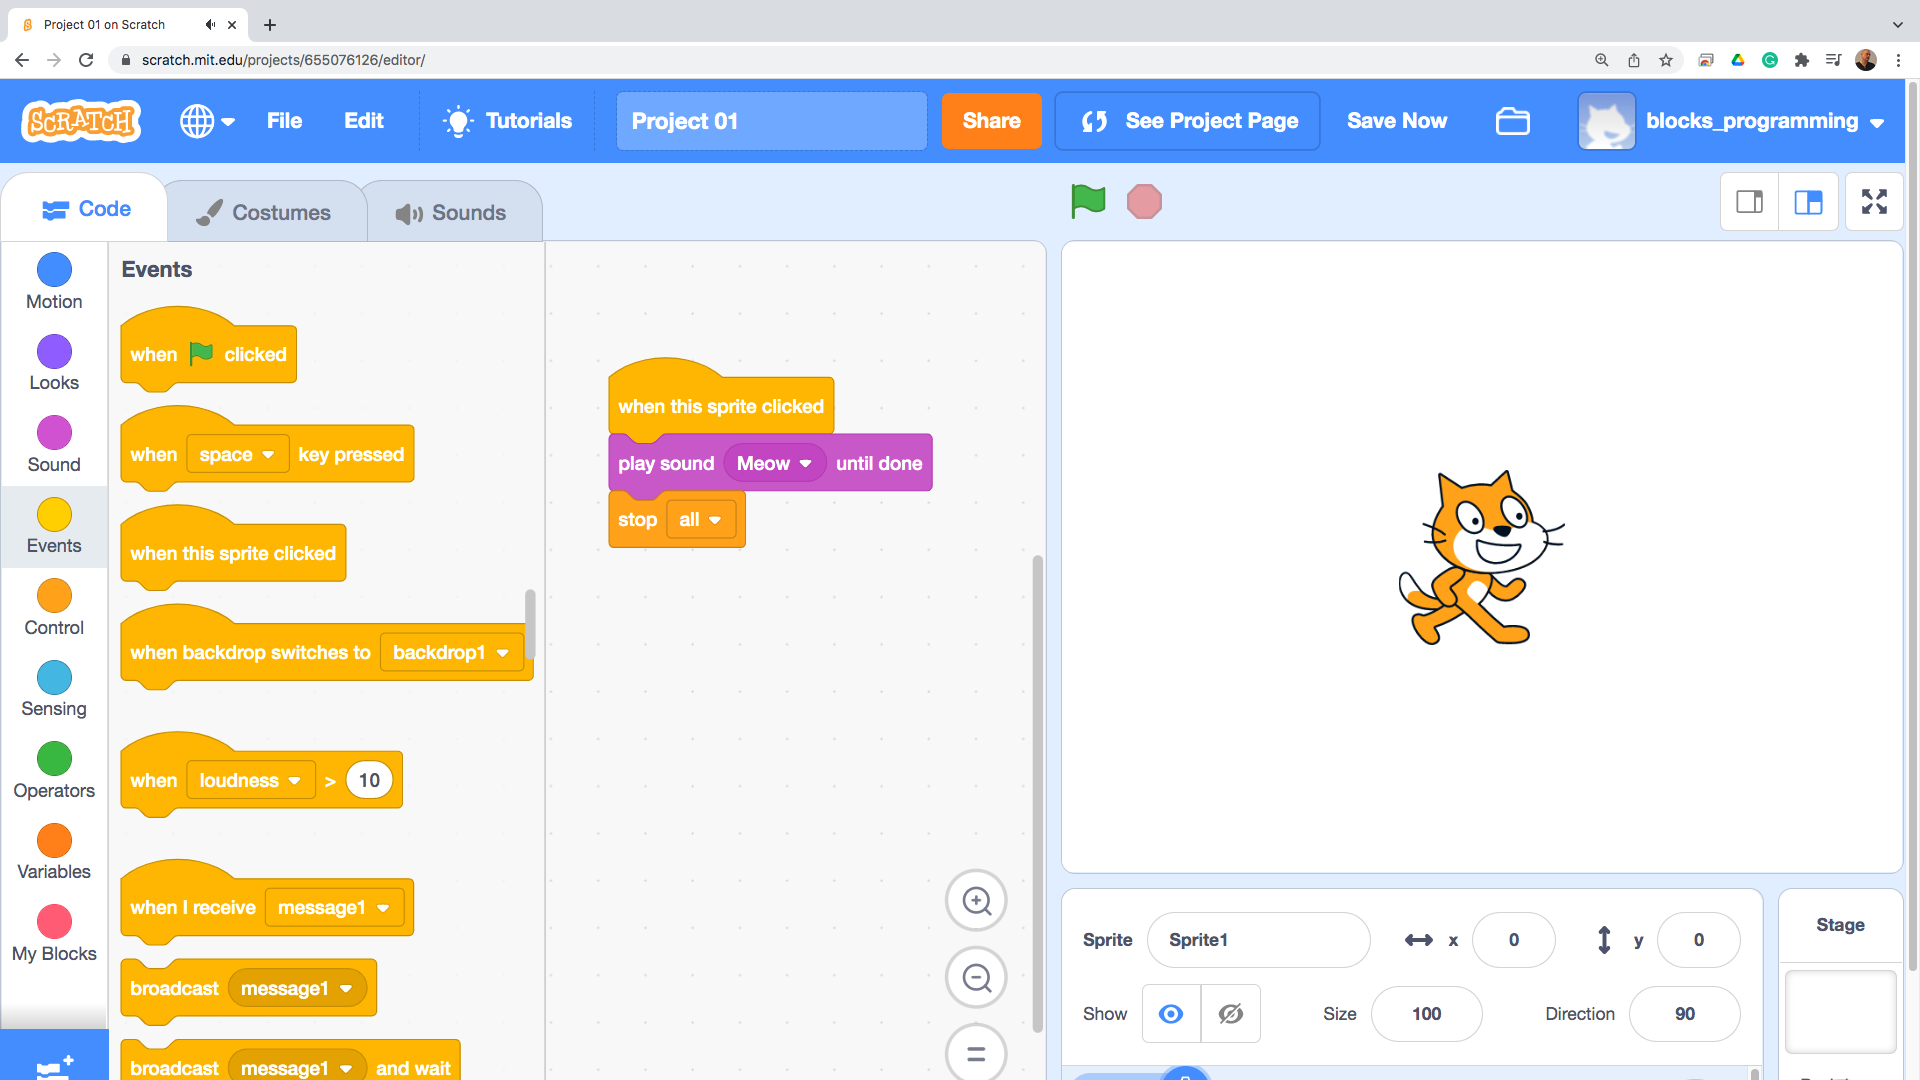
\includegraphics[width=1.0\linewidth,height=0.5\linewidth]{fig020030.png}
   \caption{Mouse Click Event}
\label{fig020030}
\end{figure}

Changing the background can also trigger an event to be handled in Scratch. For this purpose, a specific block is provided (Fig. \ref{fig020031}). 

Using this block, you can define instructions that should be executed when the background changes. This allows you to create dynamic and interactive scenes in your Scratch project.

When you connect this block to your script, it acts as an event listener, detecting changes to the background and triggering the associated instructions. This can be useful for creating transitions between different scenes or levels in a game, responding to user input, or implementing any behavior that should be triggered when the background changes.

Combining the background change event block with other blocks and instructions creates more complex interactions and effects. For example, you can change the appearance of sprites, play sounds, or initiate animations when the background is changed.

Using the background change event block adds an extra layer of interactivity and visual storytelling to your Scratch projects. It allows you to create dynamic and immersive experiences for your users.

Experiment with different backgrounds and associated events to create engaging and captivating projects in Scratch.

\begin{figure}[H]
   \centering
   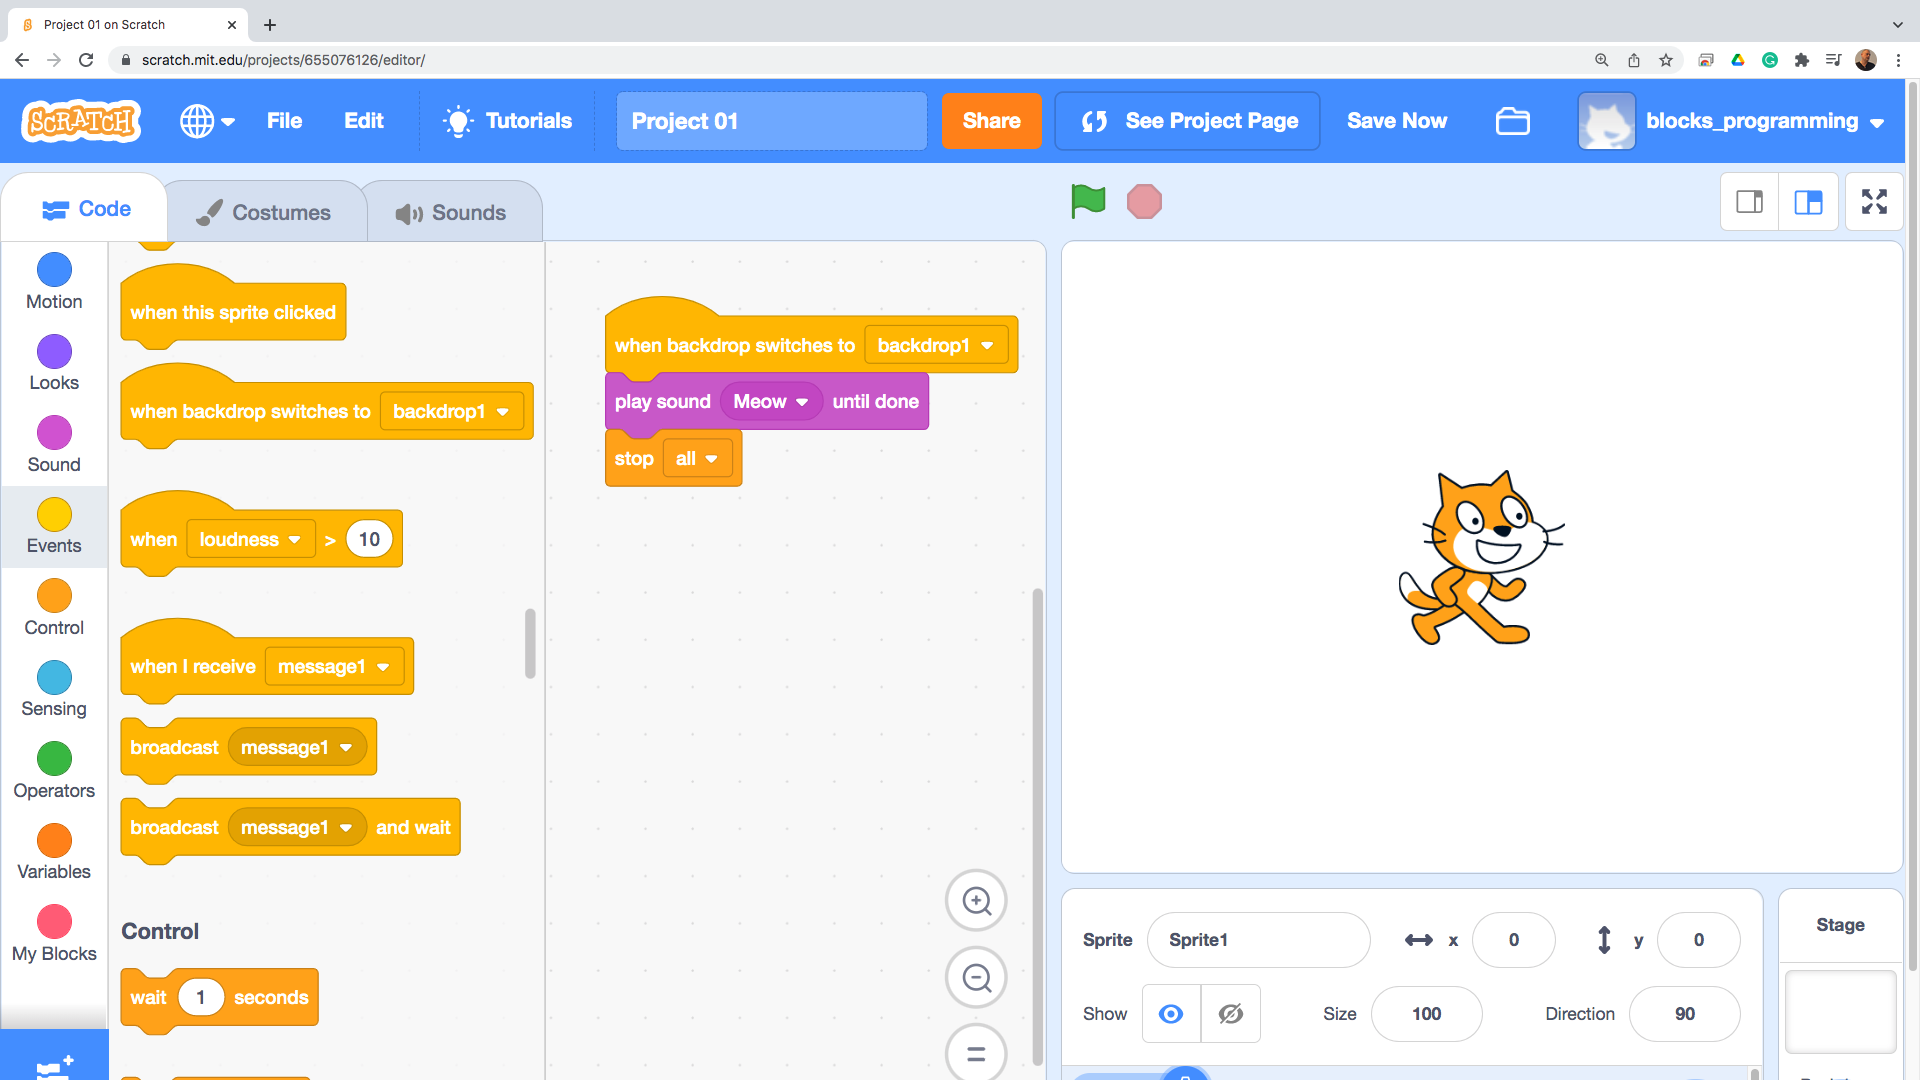
\includegraphics[width=1.0\linewidth,height=0.5\linewidth]{fig020031.png}
   \caption{BackgroundChange Event}
\label{fig020031}
\end{figure}

In Scratch, you can catch an event after a specific time or when a certain sound level has been reached. To handle such events, particular blocks are available (Fig. \ref{fig020032}).

The first block, the timer event block, allows you to define instructions that will be executed after a specified time. Connecting this block to your script can create delays or time-based actions in your project. For example, you can wait a few seconds before displaying a message or triggering an animation.

The second block, the sound level event block, enables you to react to changes in the sound level captured by the computer's microphone. You can set a threshold value, and when the sound level surpasses that threshold, the associated instructions will be executed. This can be used to create interactive projects that respond to sound or voice input.

You can introduce time-based or sound-based interactions in your Scratch projects using these event blocks. It adds a dynamic and responsive element to your creations, making them more engaging and interactive for users.

Experiment with different time intervals or sound levels to trigger different actions and create unique experiences. Combine these event blocks with other Scratch functionalities like animations, sounds, and sprites to build captivating projects that respond to various inputs.

Remember to test and iterate on your projects to fine-tune the timing or sound thresholds to achieve the desired effects. Have fun exploring the possibilities of time-based and sound-based events in Scratch!

\begin{figure}[H]
   \centering
   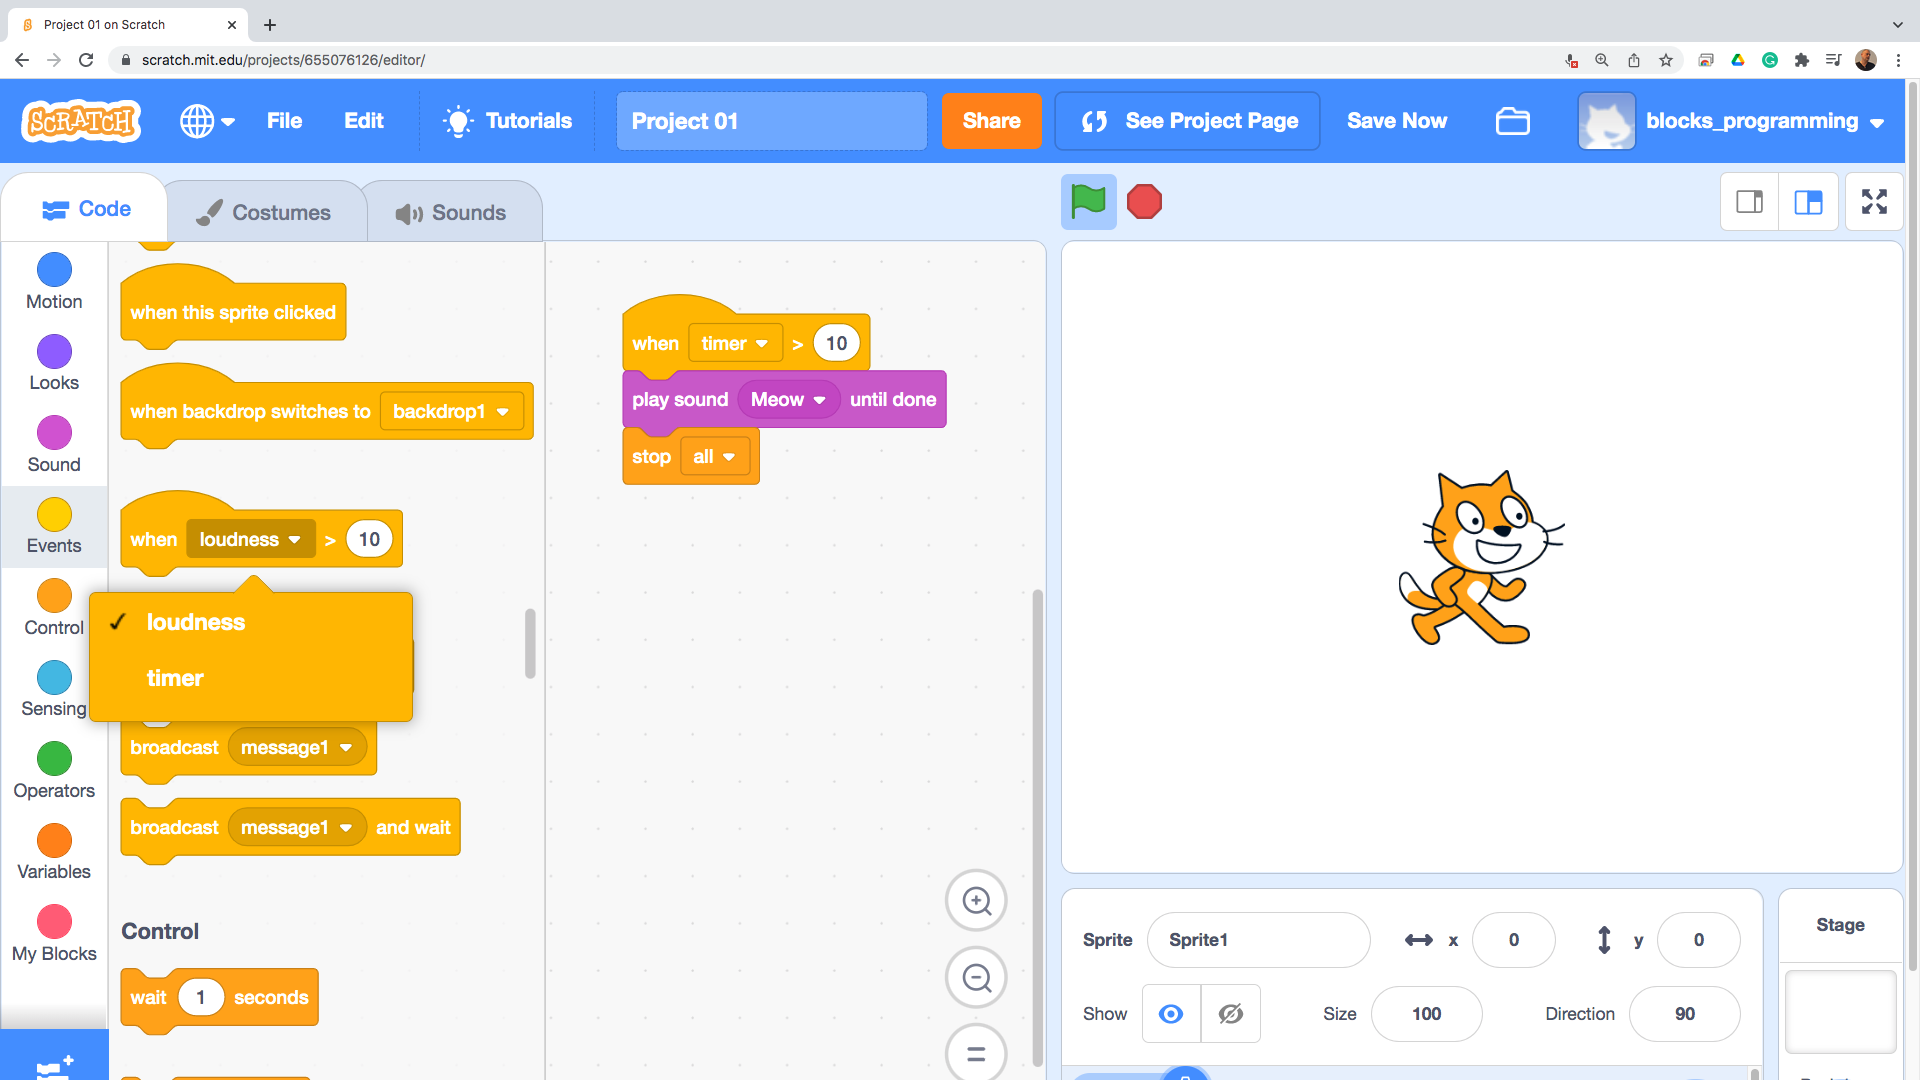
\includegraphics[width=1.0\linewidth,height=0.5\linewidth]{fig020032.png}
   \caption{Timer or sound event}
\label{fig020032}
\end{figure}

In Scratch, event handling is not limited to predefined events or inputs like keyboard or mouse interactions. It also includes a mechanism for sending and receiving messages between different parts of your project. 

To facilitate message-based communication, two specific blocks are available (Fig. \ref{fig020033}). The first block, the "broadcast" block, allows you to send a predefined message to other parts of your project. When executing this block, it triggers the corresponding event wherever the subscribed blocks are placed.

The second block, the "when I receive" block, acts as a listener for a specific message. By connecting this block to your script and specifying the desired message, you can define instructions that will be executed only when that message is received.

This message-based event-handling system enables different parts of your project to communicate and coordinate their actions. It allows you to create interactive scenarios where one sprite or script triggers actions in other sprites or scripts.

You can use messages to synchronize animations, trigger responses, or create interactive game mechanics. For example, you can have a "start" sprite broadcast a "game over" message when a certain condition is met, and other sprites can listen to that message to respond accordingly.

You can build more complex and interconnected projects in Scratch by leveraging message passing. It promotes modularity and allows for decoupled communication between different components, making your code more organized and maintainable.

Experiment with different messages and their subscriptions to create dynamic interactions within your project. Test how different sprites or scripts respond to specific messages and explore the possibilities of synchronized actions and event-driven behaviors.

Remember to give meaningful names to your messages to ensure clarity and avoid conflicts. Also, be mindful of the timing and order of message broadcasts and receptions to achieve the desired behavior.

Enjoy exploring the power of message-based event handling in Scratch and unleash your creativity in building interactive experiences!

\begin{figure}[H]
   \centering
   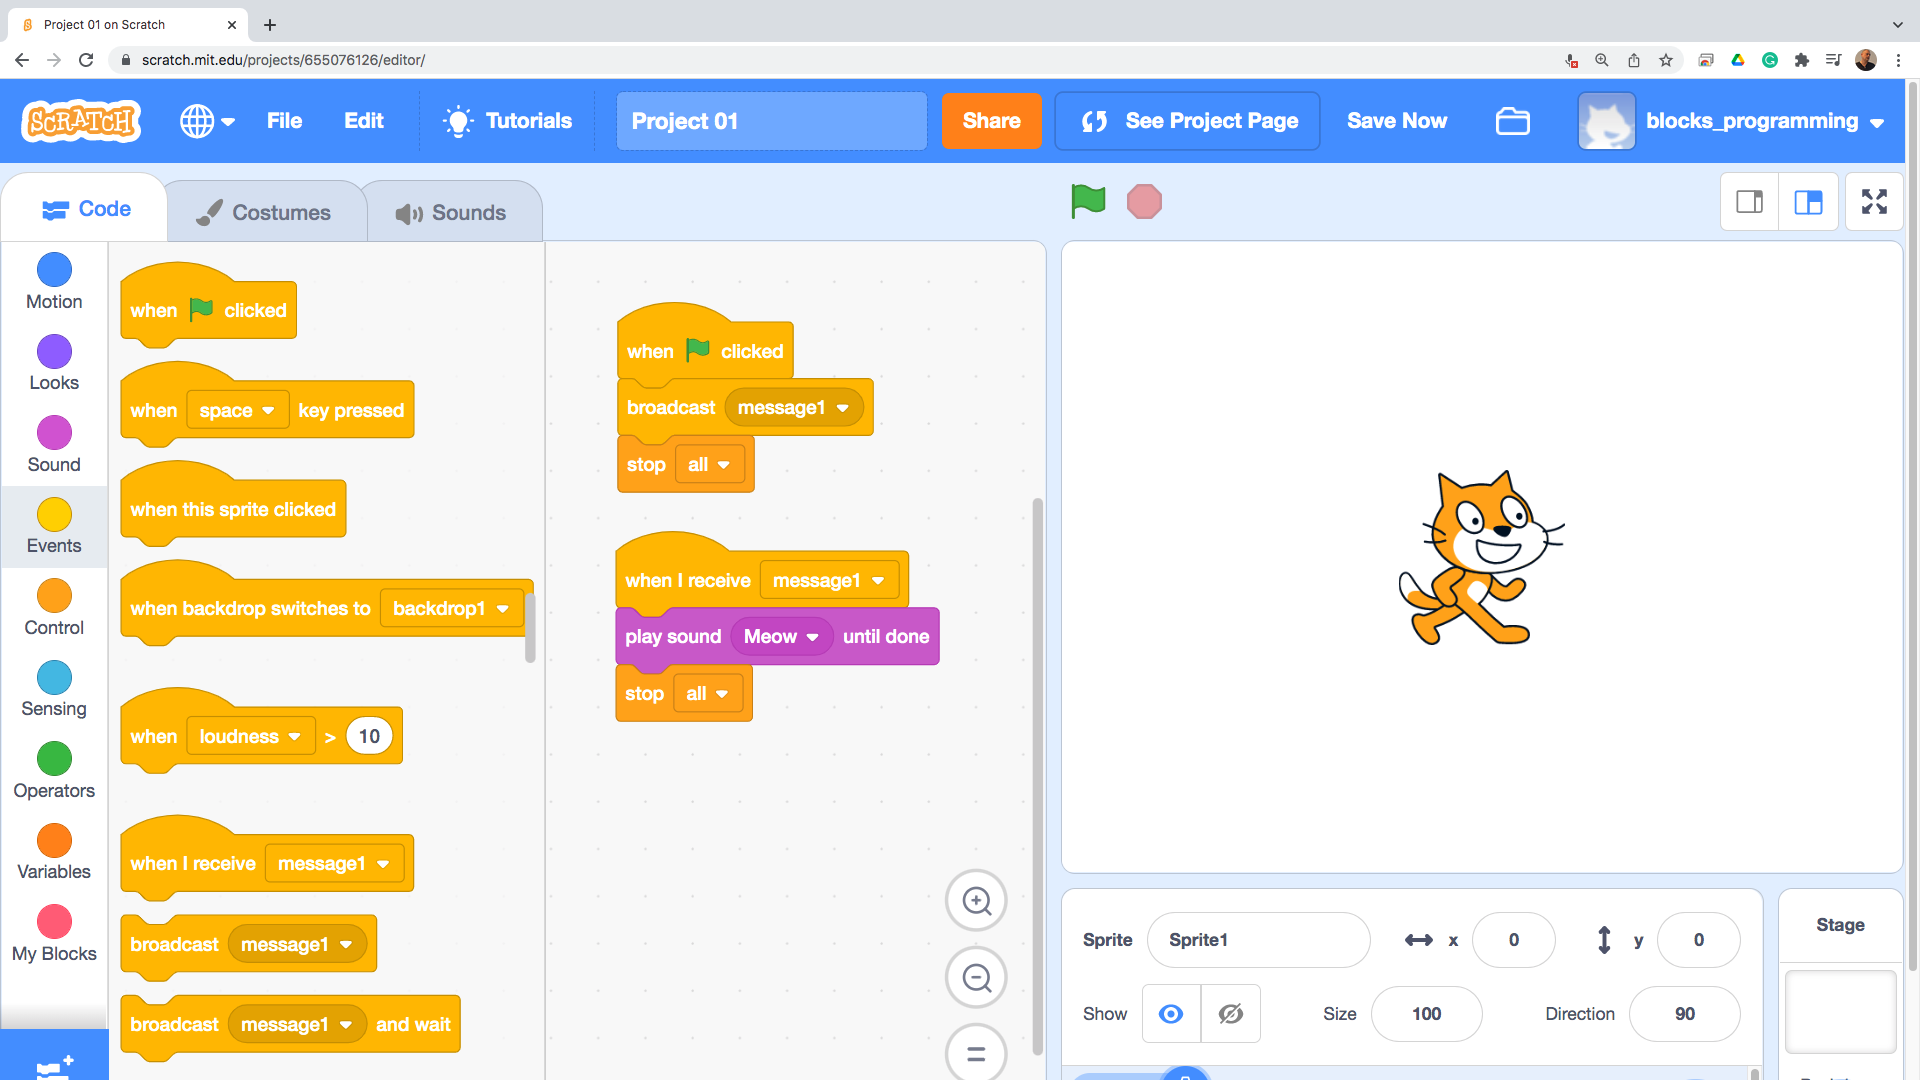
\includegraphics[width=1.0\linewidth,height=0.5\linewidth]{fig020033.png}
   \caption{Broadcasting and receiving messages}
\label{fig020033}
\end{figure}

In Scratch, working with the messaging engine sometimes requires synchronization between different parts of your project. To facilitate this, a specific block allows you to send a message and wait for a corresponding action to be taken upon its interception (Fig. \ref{fig020034}).

This block, known as the "broadcast and wait" block, combines the broadcast and wait operations. When this block is executed, it sends a message to other parts of your project, just like the regular broadcast block. However, it also pauses the execution of the current script until a response is received or the corresponding event is triggered.

Using the "broadcast and wait" block, you can ensure that the actions dependent on the message are carried out in the desired order and timing. It allows for synchronization between different sprites or scripts, ensuring they respond appropriately to the message.

You can create and define different messages for various situations as a programmer. These messages can represent different events, commands, or signals within your project. By carefully designing your messages, you can establish clear communication pathways and enable specific behaviors in response to each message.

When using the "broadcast and wait" block, it's essential to consider the flow of your program and how the different parts interact. Ensure the scripts listening for the message are appropriately positioned and ready to respond. Also, be mindful of potential delays or timeouts if the expected action is not taken within a specified time frame.

Experiment with different combinations of messages and corresponding actions to create complex and interactive behaviors in your Scratch project. Test the synchronization between other parts of your project and fine-tune the timing of message-based interactions to achieve the desired results.

With the messaging engine and the "broadcast and wait" block, you have a powerful tool to orchestrate synchronized actions and facilitate communication between different elements of your Scratch project. Use it creatively to enhance the interactivity and functionality of your projects.

\begin{figure}[H]
   \centering
   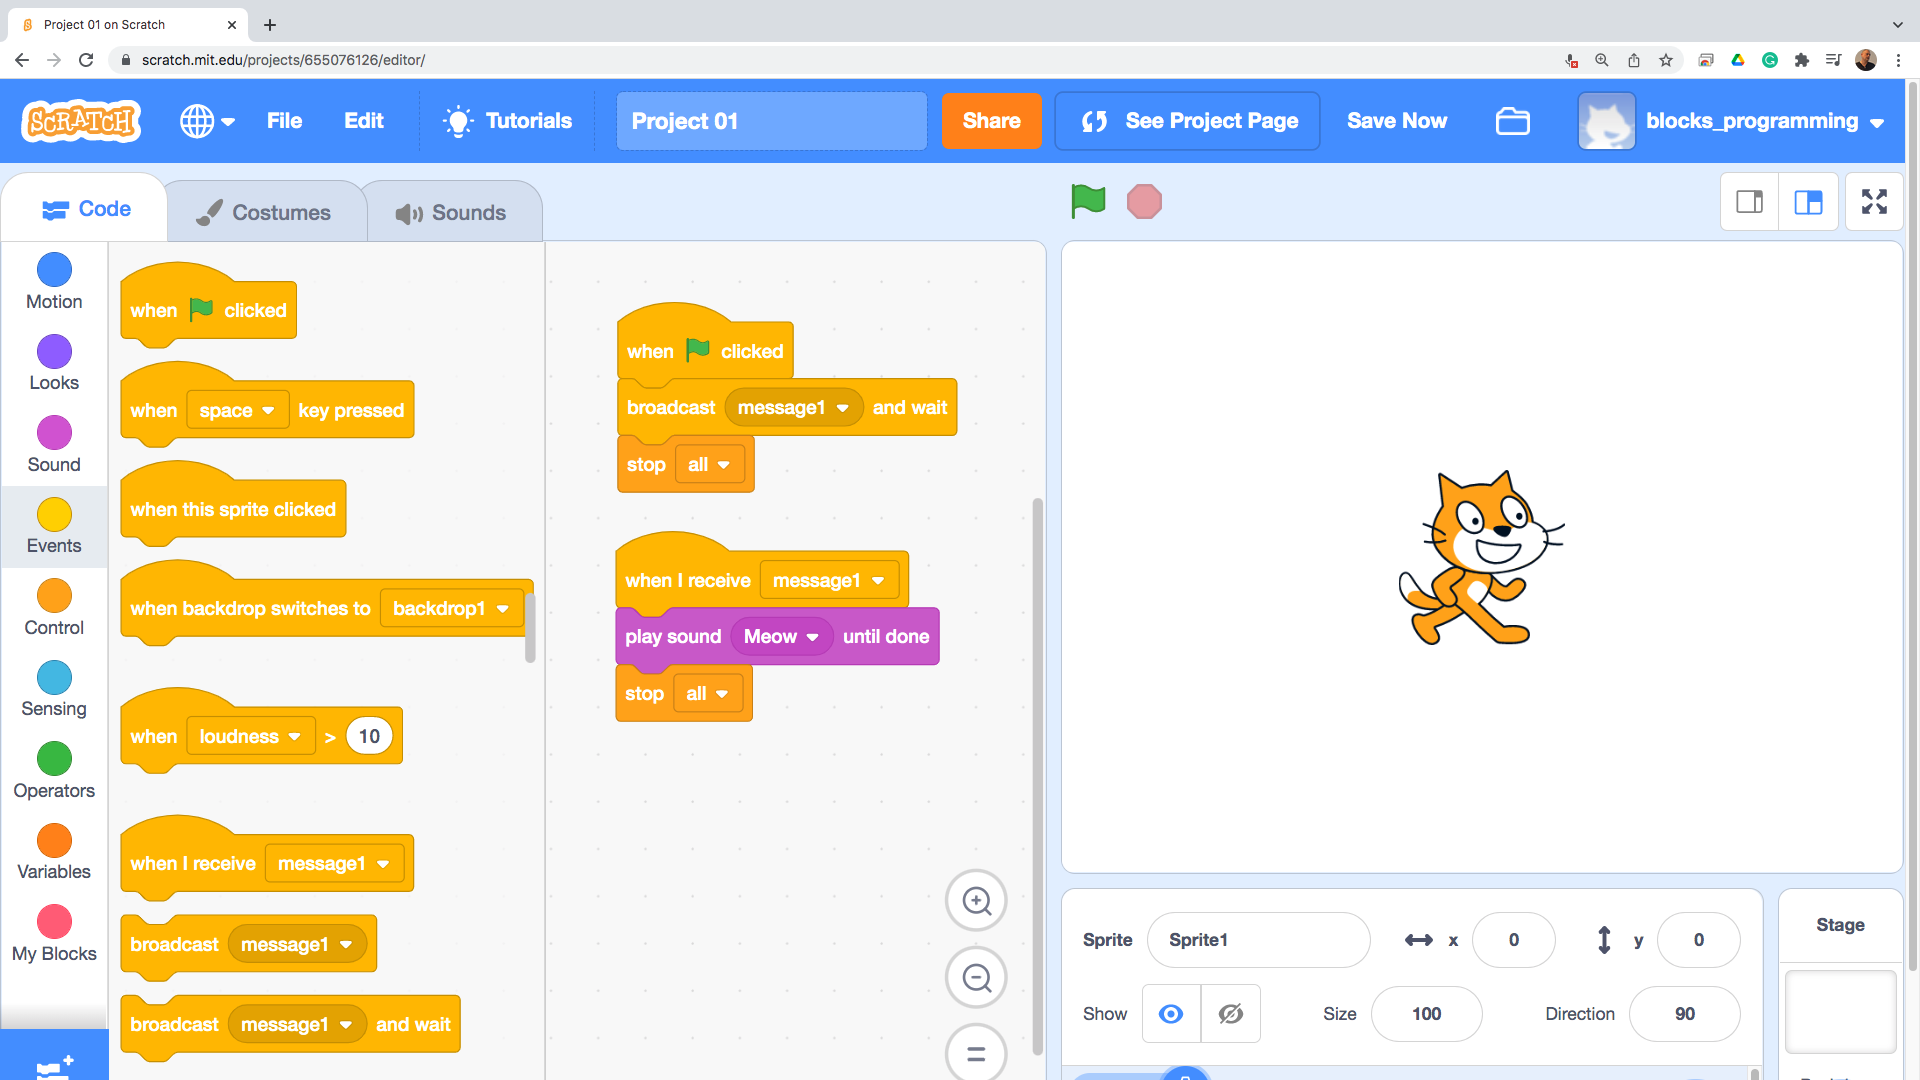
\includegraphics[width=1.0\linewidth,height=0.5\linewidth]{fig020034.png}
   \caption{Propagating a pending message}
\label{fig020034}
\end{figure}

The dark orange group in Scratch contains some of the most essential and useful blocks for controlling the execution flow of instructions. These blocks allow you to decide and choose different paths based on specific conditions. Among these blocks, there is one handy block for performing a particular action repeatedly for a set number of times (Fig. \ref{fig020035}).

In programming, the concept of repeating instructions multiple times is achieved through loop constructs. The iteration block in Scratch provides a convenient way to implement loops within your program. Using this block, you can specify the number of times you want a specific action or set of steps to be repeated.

To use the iteration block effectively, you can place the instructions you want to repeat inside the loop, ensuring they are executed the desired number of times. This is especially useful when you have a task that needs to be performed repeatedly, such as drawing a pattern, calculating a sum, or animating a sequence of movements.

You can control the exact number of repetitions by setting the appropriate value within the iteration block. This gives you precise control over how many times the actions are executed, allowing you to fine-tune the behavior of your program.

The iteration block in Scratch provides a structured and efficient way to handle repetitive tasks. It helps you avoid duplicating code and promotes cleaner and more manageable programs. Using loops, you can write more concise and expressive code that is easier to understand and maintain.

Explore the possibilities of the iteration block in Scratch, and experiment with different values to achieve the desired number of repetitions for your actions. This will allow you to create more dynamic and interactive projects where certain behaviors are repeated according to your specifications.

Remember to use loops judiciously and consider the impact they may have on the overall performance of your program. Be mindful of any potential infinite loops and ensure your loop condition is appropriately defined to avoid unintended consequences.

With the iteration block, you have a powerful tool to control repetitive actions in your Scratch projects. Embrace its versatility and unleash your creativity to build exciting and engaging experiences.

\begin{figure}[H]
   \centering
   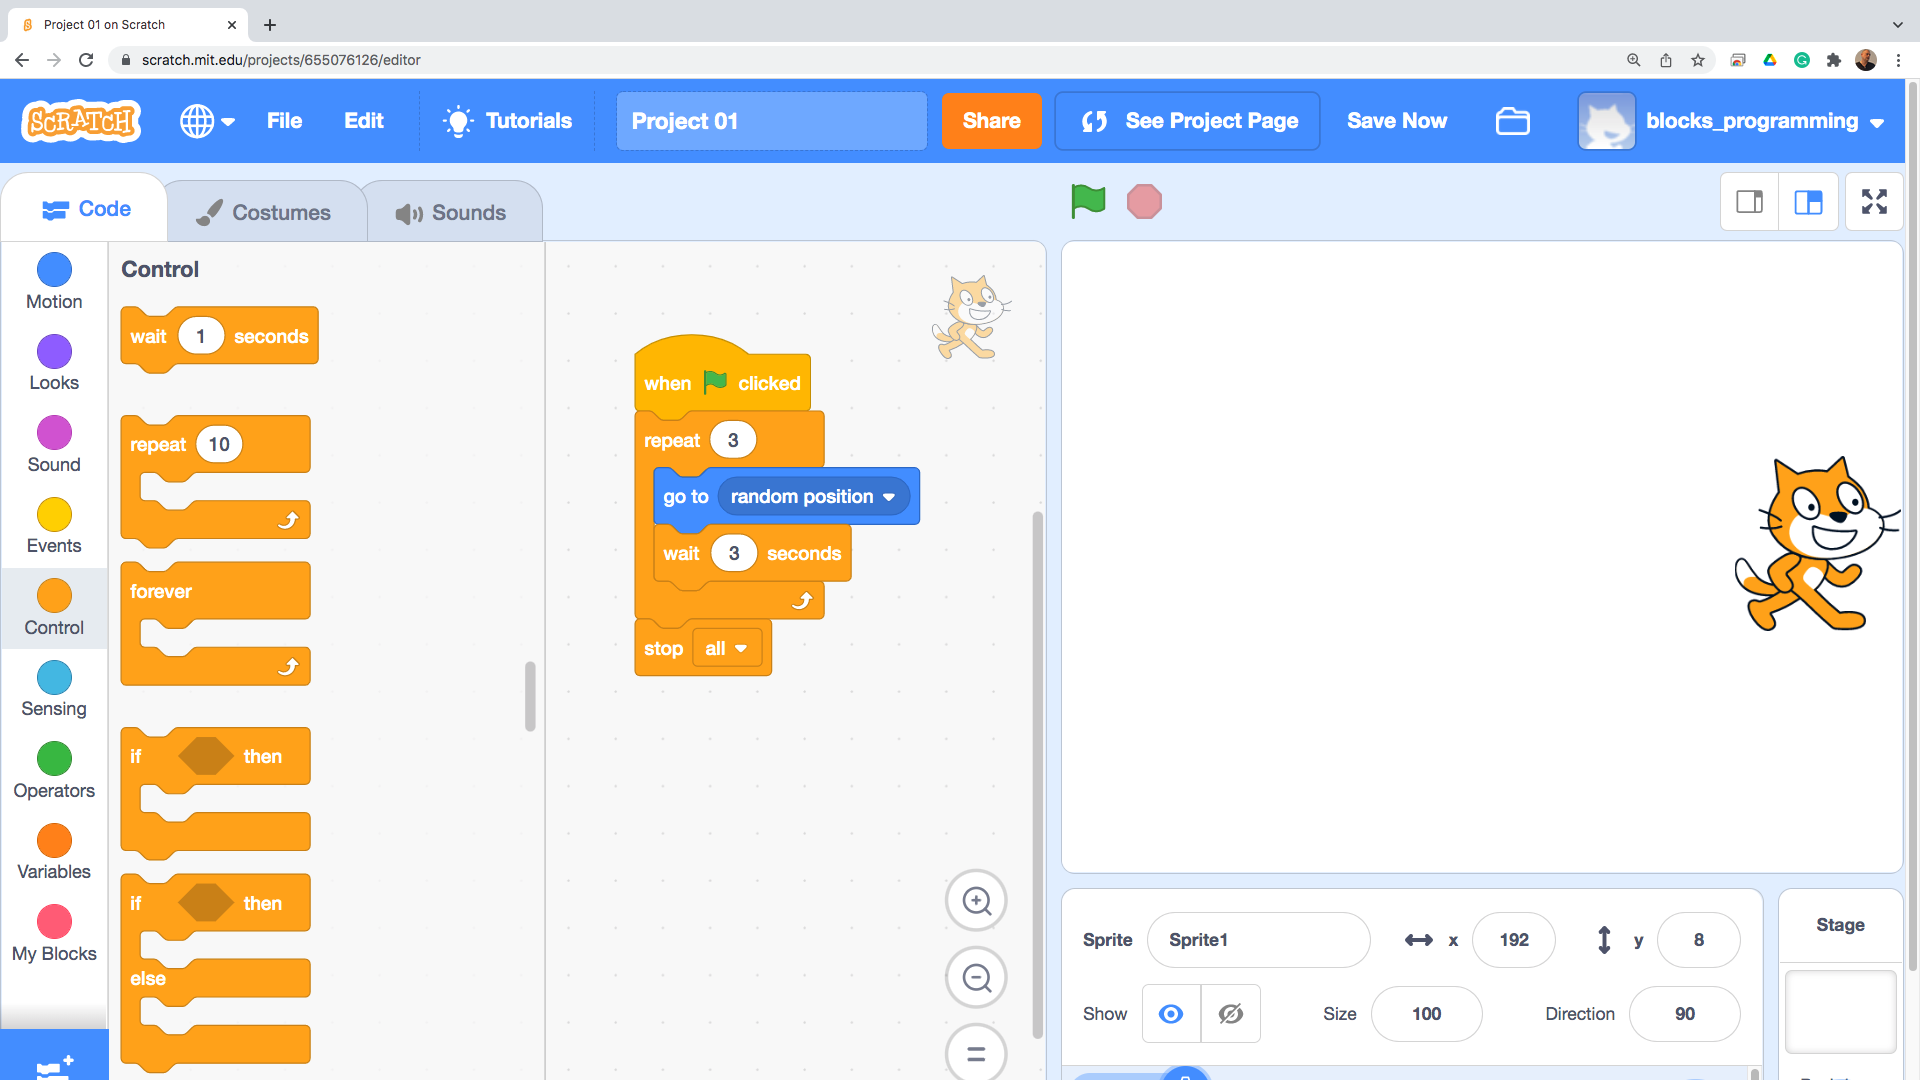
\includegraphics[width=1.0\linewidth,height=0.5\linewidth]{fig020035.png}
   \caption{Fixed number of iterations}
\label{fig020035}
\end{figure}

The "repeat" block in Scratch allows you to perform a specific set of instructions repeatedly for a certain number of times. As the name suggests, the block's purpose is to repeat a sequence of actions. The numerical input inside the block determines how many repetitions will be executed, while the space inside is where you place the instructions to be repeated. 

For instance, let's consider an example where a sprite, such as a kitten, is moved to randomly selected coordinates, and then a pause of a specified duration is inserted. Using the "repeat" block, you can easily instruct the program to execute this sequence of actions multiple times.

The "repeat" block is a valuable tool to avoid duplicating the exact instructions manually. Instead, you can encapsulate the repetitive actions within the block, making your code more concise and easier to manage.

Sometimes, you may encounter situations where an infinitely repeating loop is needed. While using infinite loops with caution is essential, Scratch provides a specific block to handle such scenarios (Fig. \ref{fig020036}). This block allows you to create a loop that repeats indefinitely until certain conditions are met or until the user stops the program.

When using infinite loops, it is crucial to ensure an appropriate exit condition to prevent the program from getting stuck in an endless loop. Careful consideration and planning are required to implement such loops effectively and avoid unintended consequences.

The "repeat" block and the "forever" block offer different ways to control the repetition of instructions in your Scratch program. By leveraging these blocks, you can create dynamic and interactive projects that respond to user input or execute specific actions several times.

Remember to experiment with different values inside the "repeat" block to achieve the desired number of repetitions. This flexibility allows you to fine-tune the behavior of your program and bring your ideas to life.

Remember that using loops effectively requires understanding their logic and structuring your code appropriately. Test and debug your program to ensure it behaves as expected and avoid potential errors or unexpected behavior.

The "repeat" and the "forever" blocks are powerful tools in Scratch that allow you to create complex and interactive projects. Embrace their capabilities and unleash your creativity to build engaging experiences for yourself and others.

\begin{figure}[H]
   \centering
   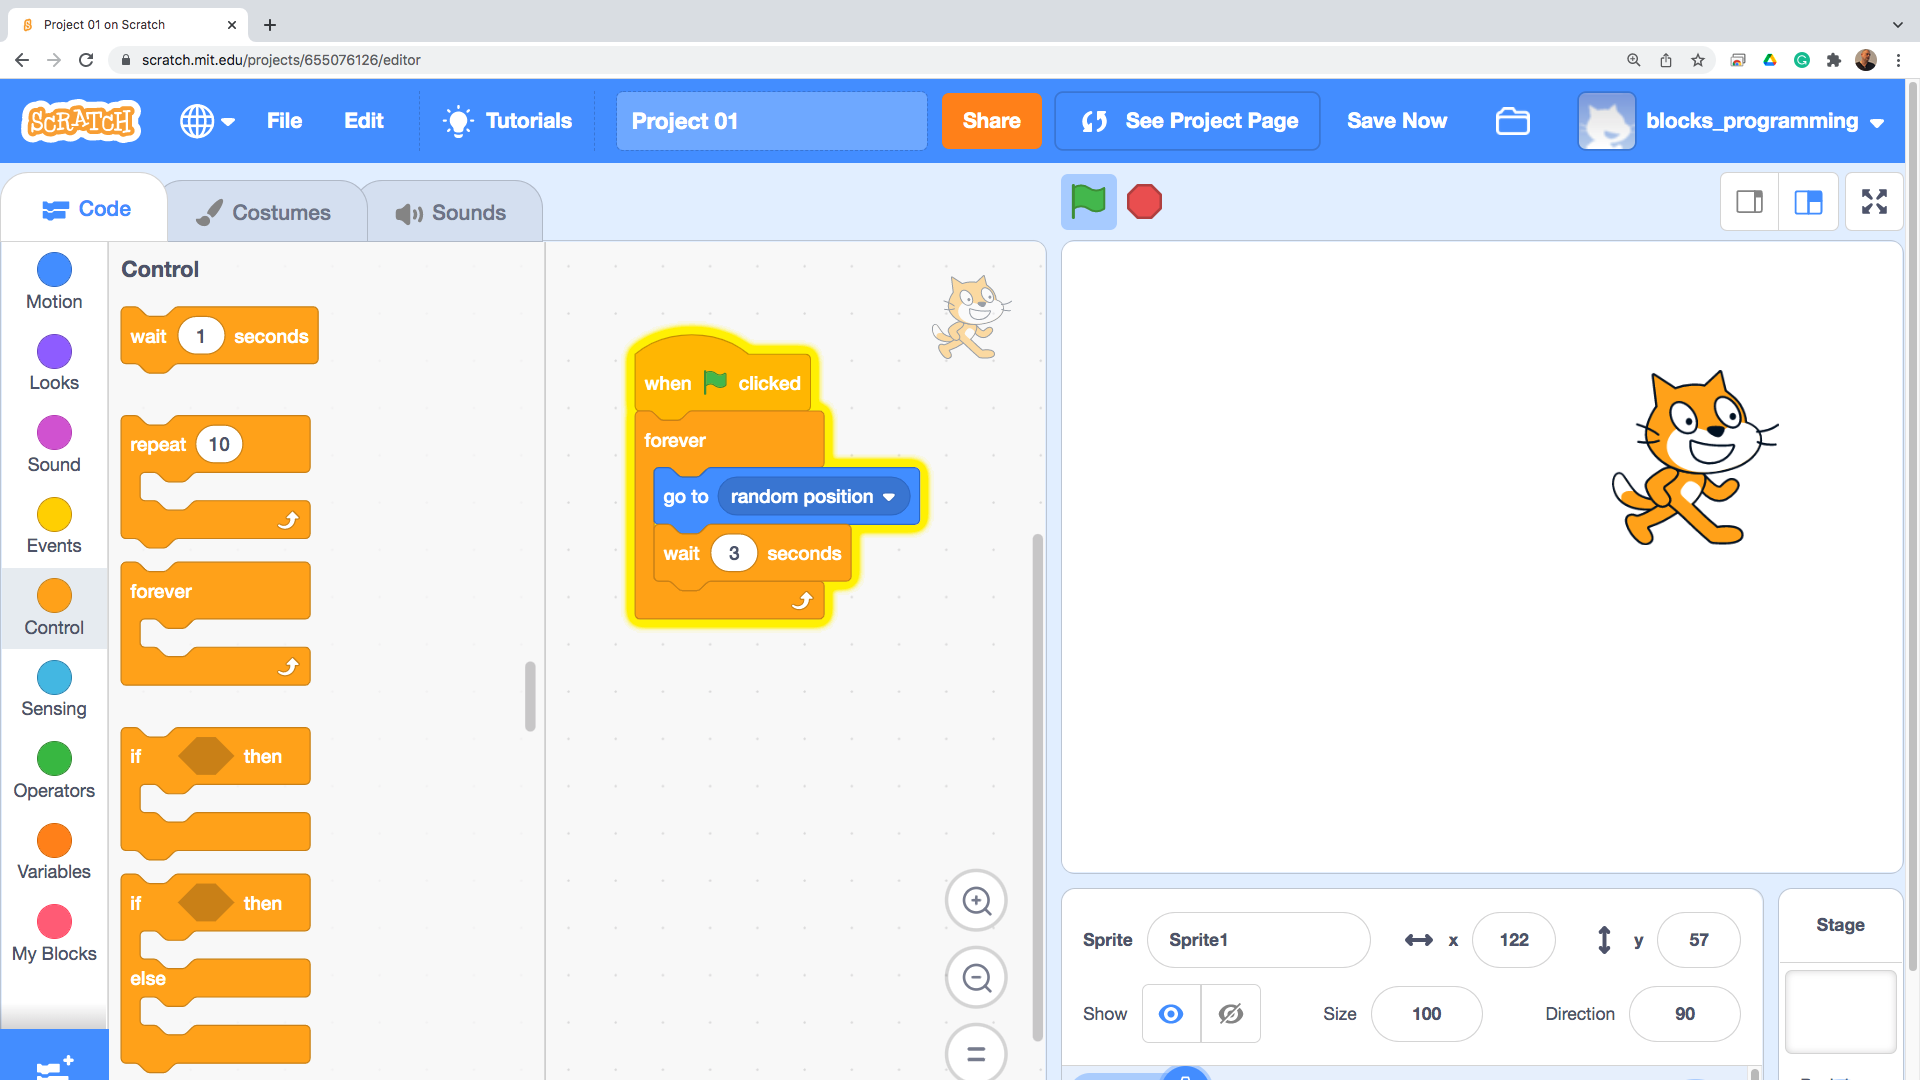
\includegraphics[width=1.0\linewidth,height=0.5\linewidth]{fig020036.png}
   \caption{Infinite Replays}
\label{fig020036}
\end{figure}

The conditional execution block, also known as a conditional statement or conditional transition, is one of the fundamental building blocks in programming (Fig. \ref{fig020037}). This block allows you to control the flow of your program based on certain conditions. The instructions inside the block are executed only if the condition specified in its header is satisfied.

Conditional statements are essential for making decisions and branching your code based on different scenarios. They enable your program to respond dynamically and adapt to varying situations. With conditional execution blocks, you can create logic that selectively executes specific actions based on the values of variables, user input, or other factors.

The condition in the block's header is typically a logical expression that evaluates to either true or false. When the condition is true, the instructions within the block are executed. If the condition is false, the instructions are skipped, and the program continues to the following sequential statement.

By using conditional execution blocks, you can incorporate different behaviors and outcomes into your program. For example, you can create branches that execute specific actions if a certain condition is met and alternative branches that perform different actions if the condition is not met.

It is essential to construct the condition accurately to ensure the desired logic of your program. You can use comparison operators (such as equal to, not equal to, greater than, less than) and logical operators (such as and, or, not) to create complex conditions that capture specific requirements.

Furthermore, conditional statements can be nested within each other to create more intricate decision-making processes. This allows you to handle multiple scenarios and fine-tune the behavior of your program based on various conditions.

Mastering conditional execution blocks is crucial for writing robust and dynamic programs. They empower you to add intelligence, interactivity, and flexibility to your projects. You can create programs that respond intelligently to different inputs and scenarios by carefully designing your conditions and defining appropriate actions.

As you gain experience, you will discover the versatility and power of conditional execution blocks in shaping the behavior and logic of your programs. Embrace this important concept, practice applying it in different situations, and continue exploring more advanced uses of conditional statements in your coding journey.

\begin{figure}[H]
   \centering
   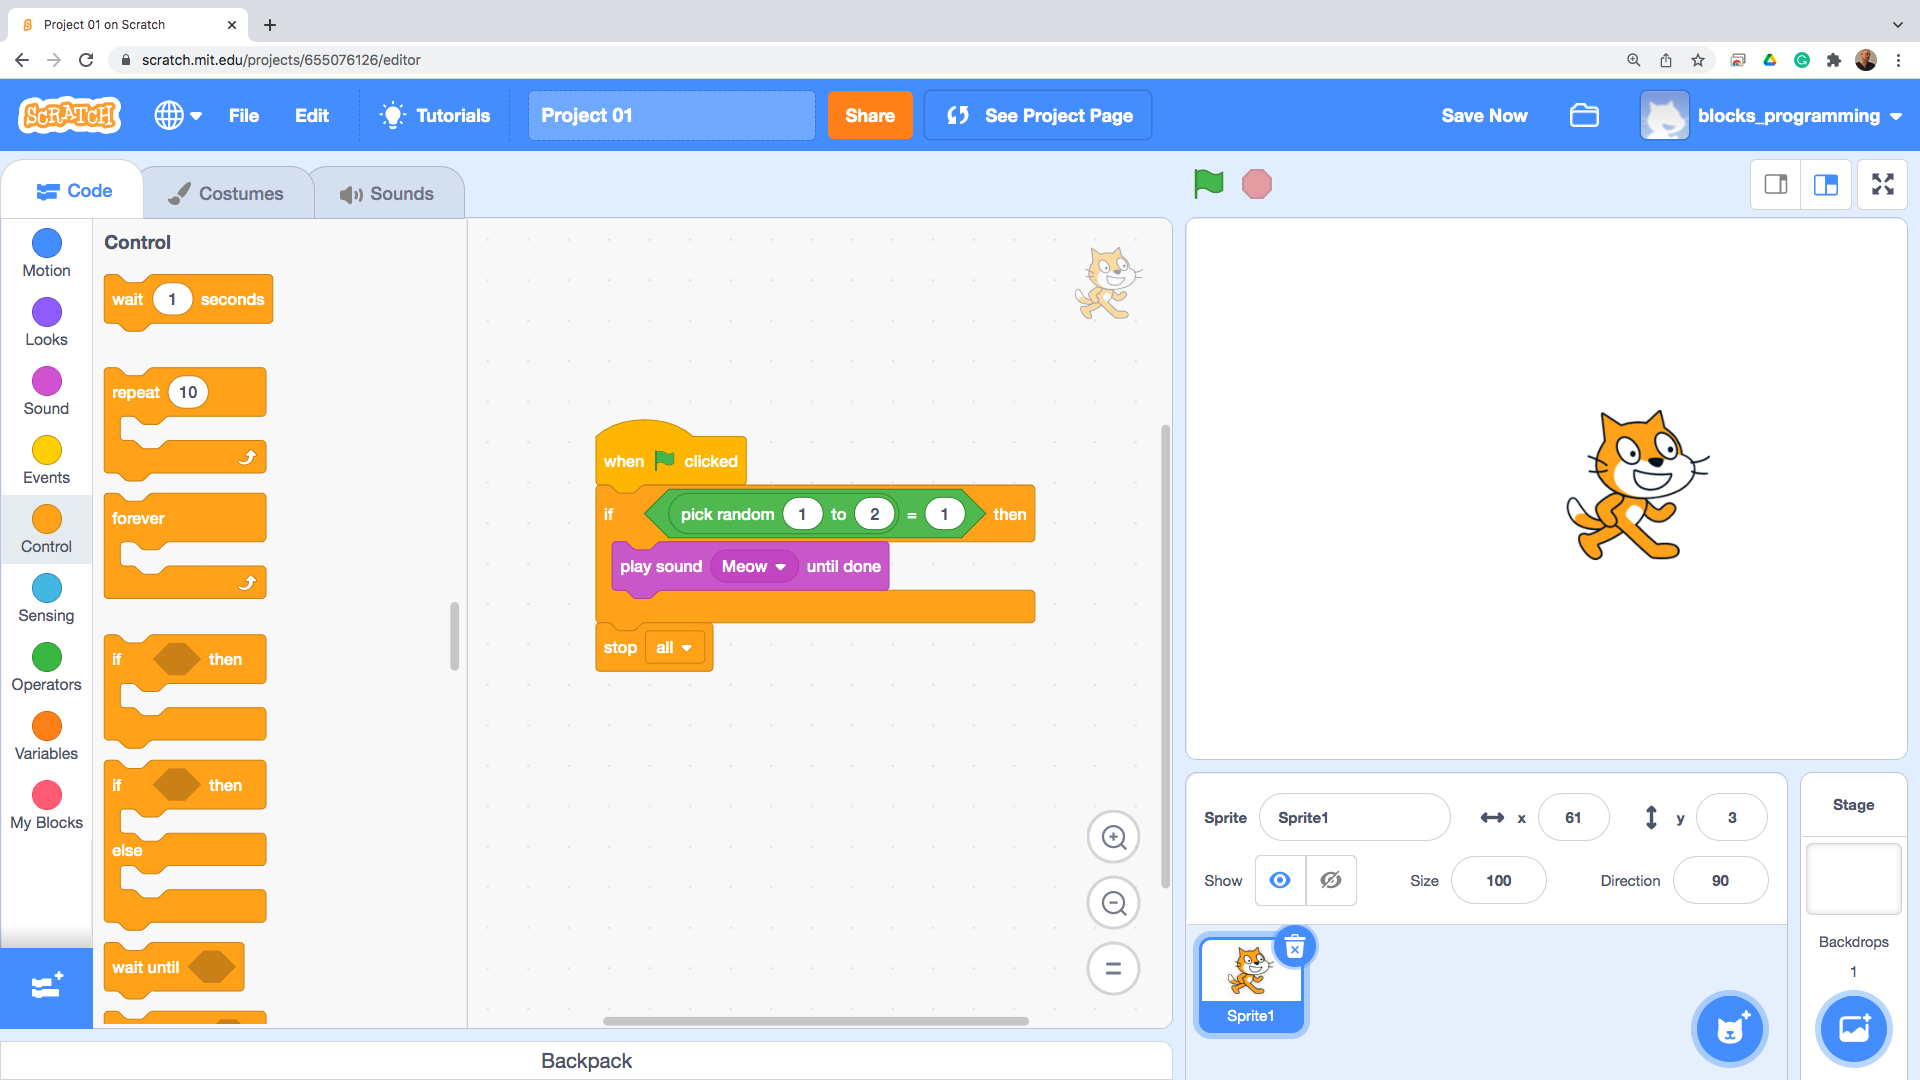
\includegraphics[width=1.0\linewidth,height=0.5\linewidth]{fig020037.png}
   \caption{Execution on condition}
\label{fig020037}
\end{figure}

The dark orange conditional execution block (Fig. \ref{fig020038}) is always used with at least one green block and sometimes two, as shown in the current example. The green blocks, shaped like irregular hexagons, are designed to fit into the header of certain dark orange blocks. These hexagonal blocks feature an oval slot where specific green oval blocks can be inserted.

In the given example, a green block that checks for equality to a specific number is selected. A random number within a predetermined range is generated to generate the value for the oval block. The condition in the header of the conditional execution block is evaluated based on these values. The instructions inside the block's body are executed if the condition is satisfied. However, if the condition is not met, the body is skipped, and the program continues with the instructions after the block.

The conditional execution block also has a variant that provides slots for executing instructions based on true and false conditions. In this variant (Fig. \ref{fig020038}), the first set of instructions is executed if the condition is true. On the other hand, if the condition is false, the second set of instructions is executed.

By utilizing conditional execution blocks, you can introduce decision-making capabilities to your program. The condition in the block's header determines which path the program takes based on the values and comparisons involved. This allows for dynamic and adaptive behavior, enabling your program to respond differently to various inputs or conditions.

Remember, proper construction of the condition is crucial for the expected behavior of your program. You can use comparison operators (e.g., equal to, not equal to, greater than, less than) and logical operators (e.g., and, or, not) to build complex conditions that accurately capture your requirements.

Through practice and experimentation, you'll gain proficiency in using conditional execution blocks effectively. They are a powerful tool for adding logic and decision-making capabilities to your projects, enabling your programs to respond intelligently and flexibly to different scenarios. Embrace the versatility of these blocks and continue exploring their applications in your programming endeavors.

\begin{figure}[H]
   \centering
   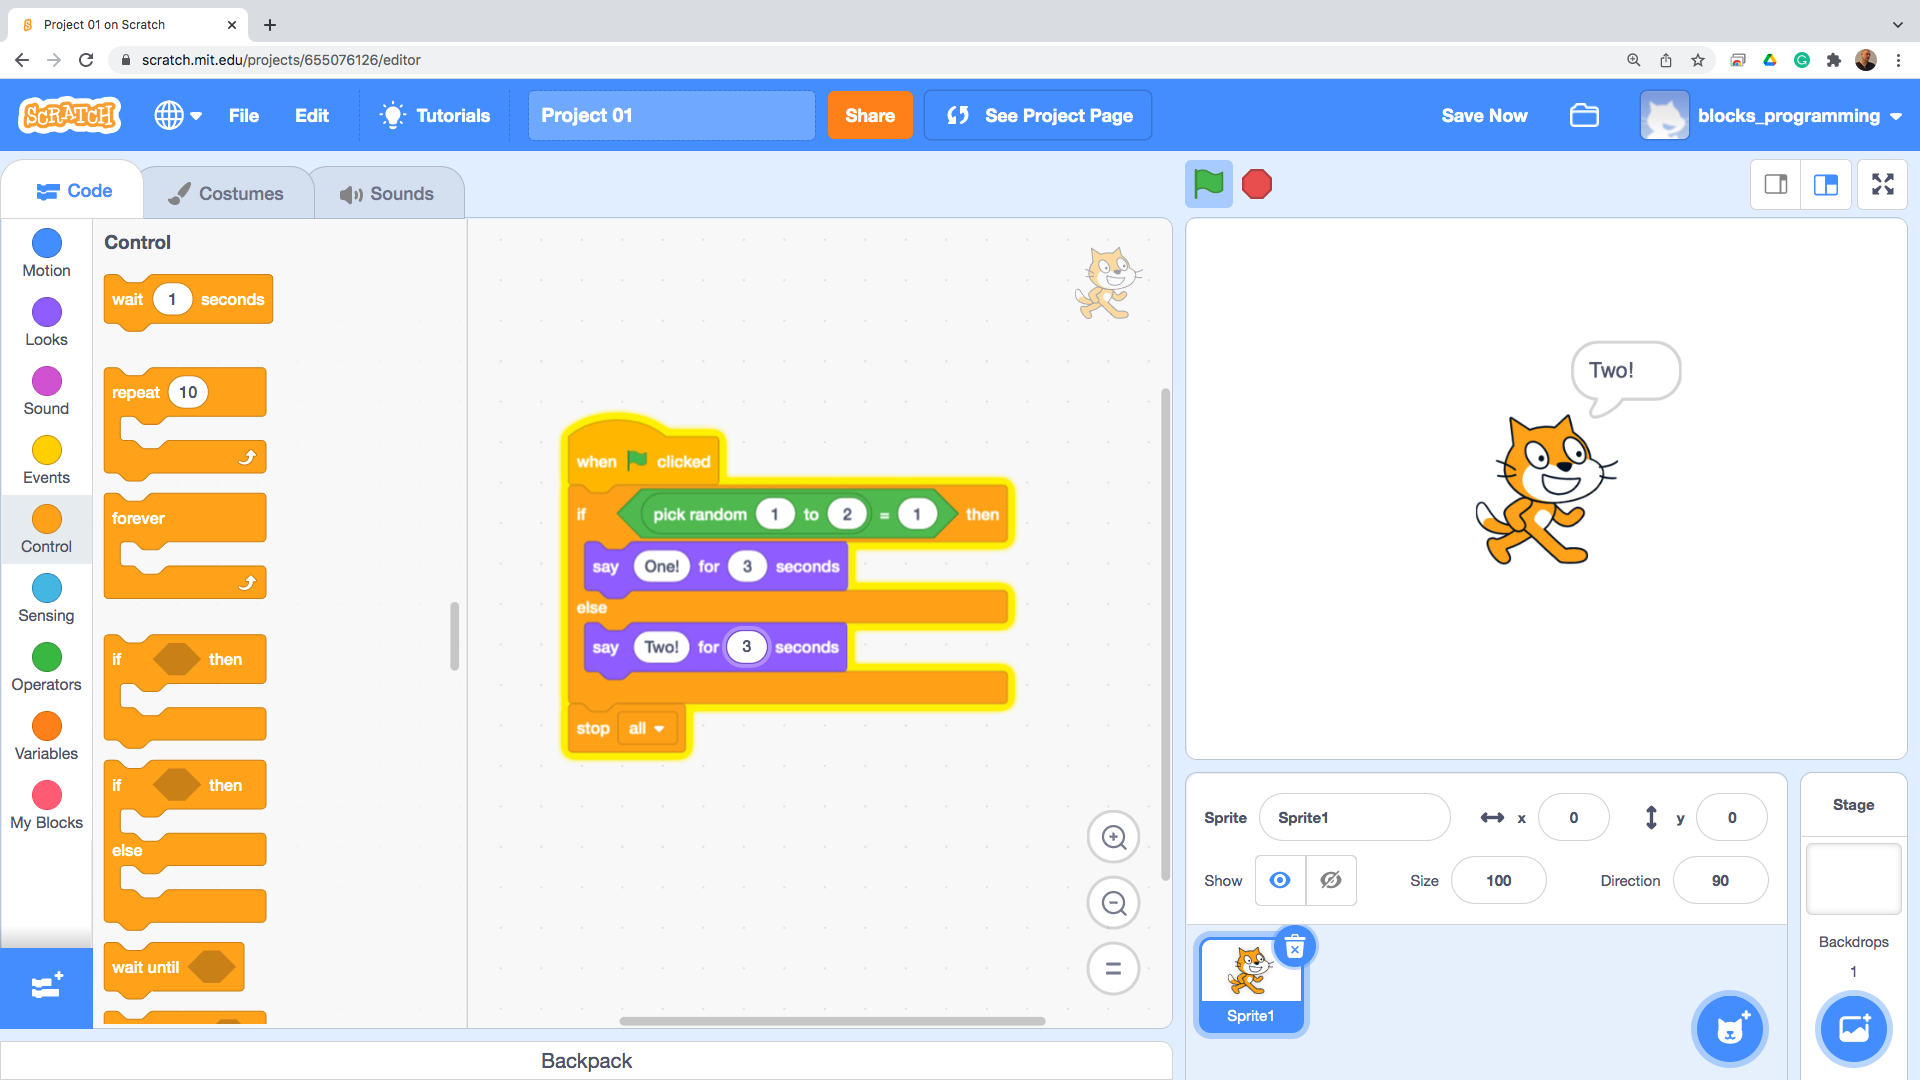
\includegraphics[width=1.0\linewidth,height=0.5\linewidth]{fig020038.png}
   \caption{Execution on condition with alternative}
\label{fig020038}
\end{figure}

The following intriguing block is the "wait until" block, which allows the program to pause execution until a specific event occurs. In this case, the event is defined as the sprite being touched with the mouse (Fig. \ref{fig020039}). When this touch event happens, the program proceeds to the next block and continues its execution.

An additional block (light blue) with an irregular hexagonal shape is used to specify the desired event. This block serves as a condition that determines when the "wait until" block should conclude. The condition can be tailored to various criteria, such as mouse interactions, key presses, or other sprite-related events.

You can create interactive and responsive programs by incorporating the "wait until" block and its associated condition block. This allows for synchronization with user actions or specific triggers, ensuring that particular instructions are executed only when the desired event occurs.

Utilize the flexibility of the condition block to define the specific event or condition that needs to be met for the program to proceed. Experiment with different event types and explore the possibilities of creating engaging and dynamic experiences through event-driven programming.

With the "wait until" block, you can introduce a level of interactivity that enables your program to wait for user input or specific conditions before moving forward. This capability allows for creating interactive games, simulations, and other engaging projects.

\begin{figure}[H]
   \centering
   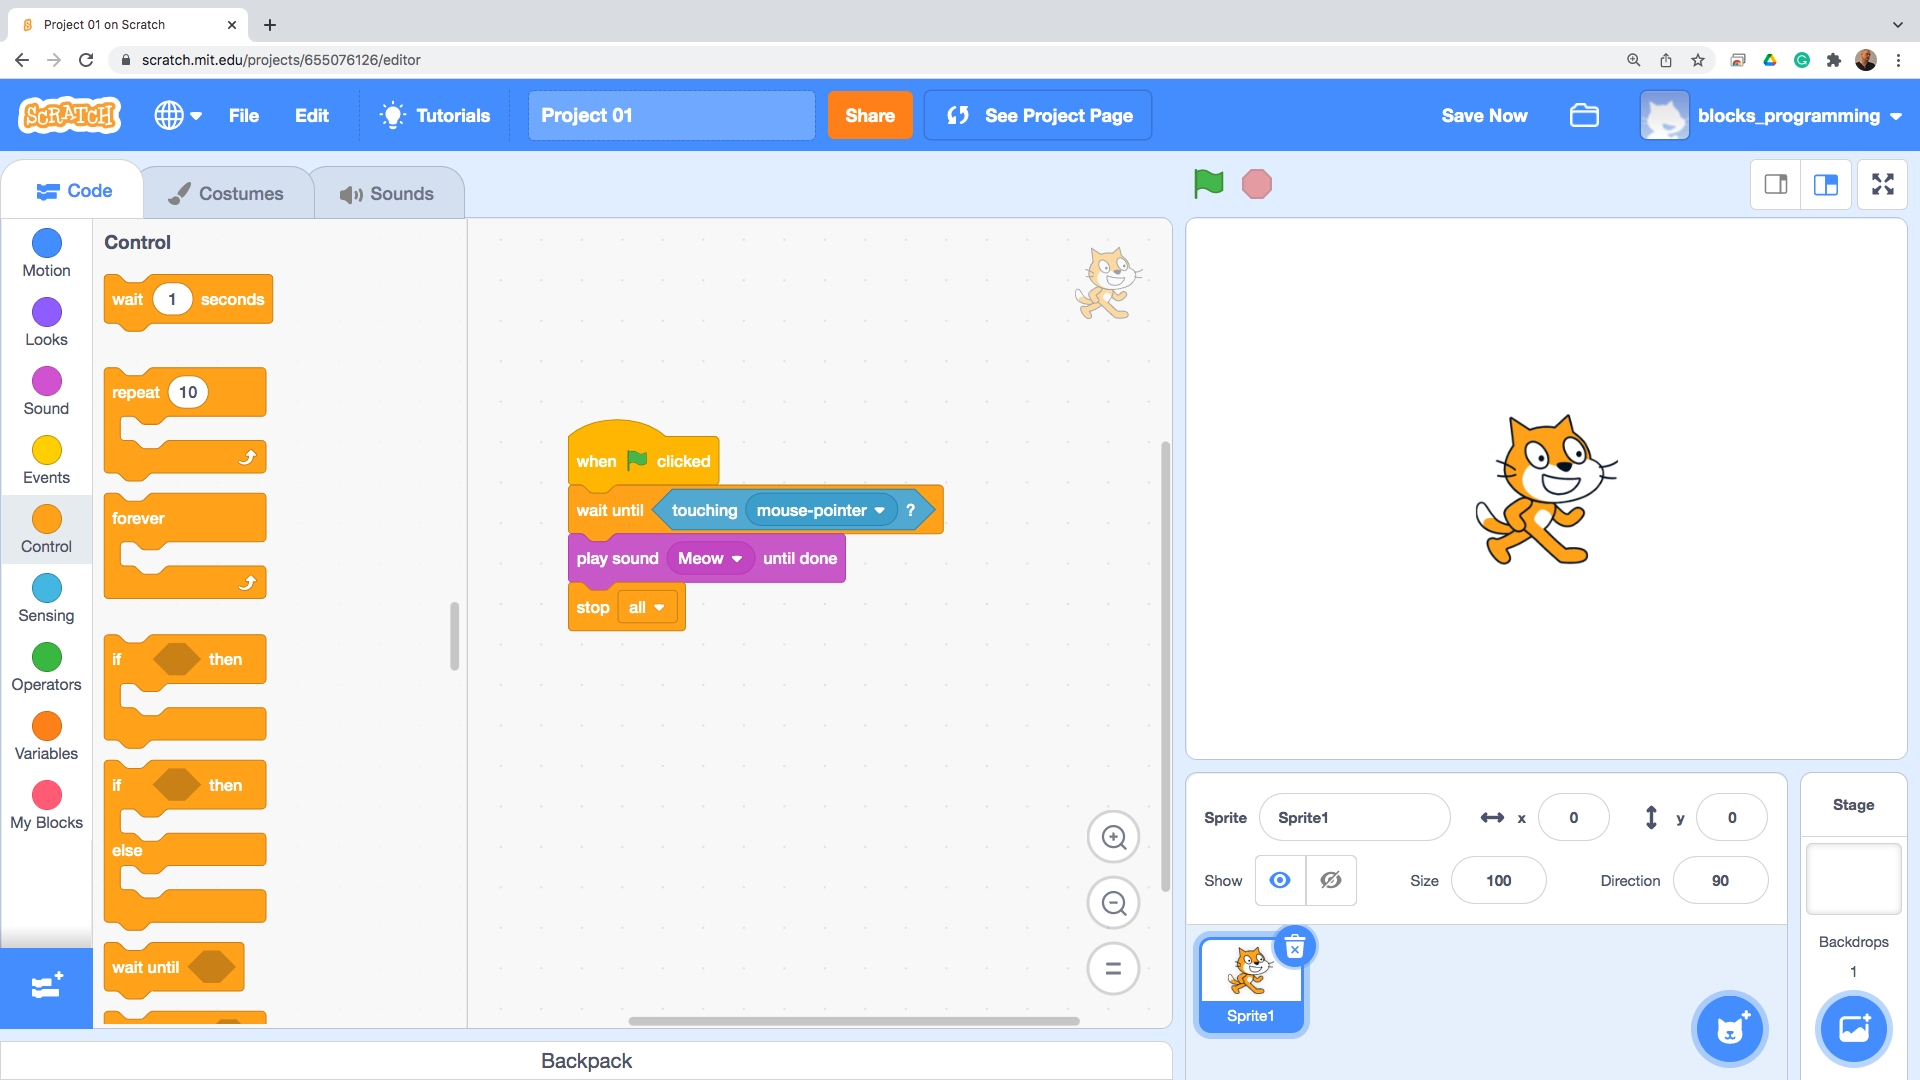
\includegraphics[width=1.0\linewidth,height=0.5\linewidth]{fig020039.png}
   \caption{Waiting condition}
\label{fig020039}
\end{figure}

The final three blocks in the dark orange group are designed to work together and demonstrate sprite cloning and deletion functionality (Fig. \ref{fig020040}). These blocks enable you to create and manage multiple sprite instances within your program.

The first block establishes a new sequence of instructions that will be executed when a specific sprite is cloned. This block allows you to define the behavior and actions of the cloned sprite independently from the original sprite.

The second block, known as the "clone" block, creates a new instance or clone of the current sprite. When this block is executed, an identical copy of the sprite is generated, including its appearance, position, and other associated attributes.

The third block lets you delete the current sprite from the scene. When this block is executed, the sprite is removed, and its associated resources are freed up. This is particularly useful when you no longer need a sprite in your program and want to remove it dynamically.

Combining these three blocks allows you to dynamically create, manage, and remove sprite clones in your project. This capability provides for creating dynamic scenes, spawning new characters, or managing game elements.

Experiment with sprite cloning and deletion to add depth and flexibility to your projects. Whether you're creating games, simulations, or interactive stories, these blocks provide you with the tools to create and manage multiple instances of sprites, enhancing the interactivity and complexity of your programs.

\begin{figure}[H]
   \centering
   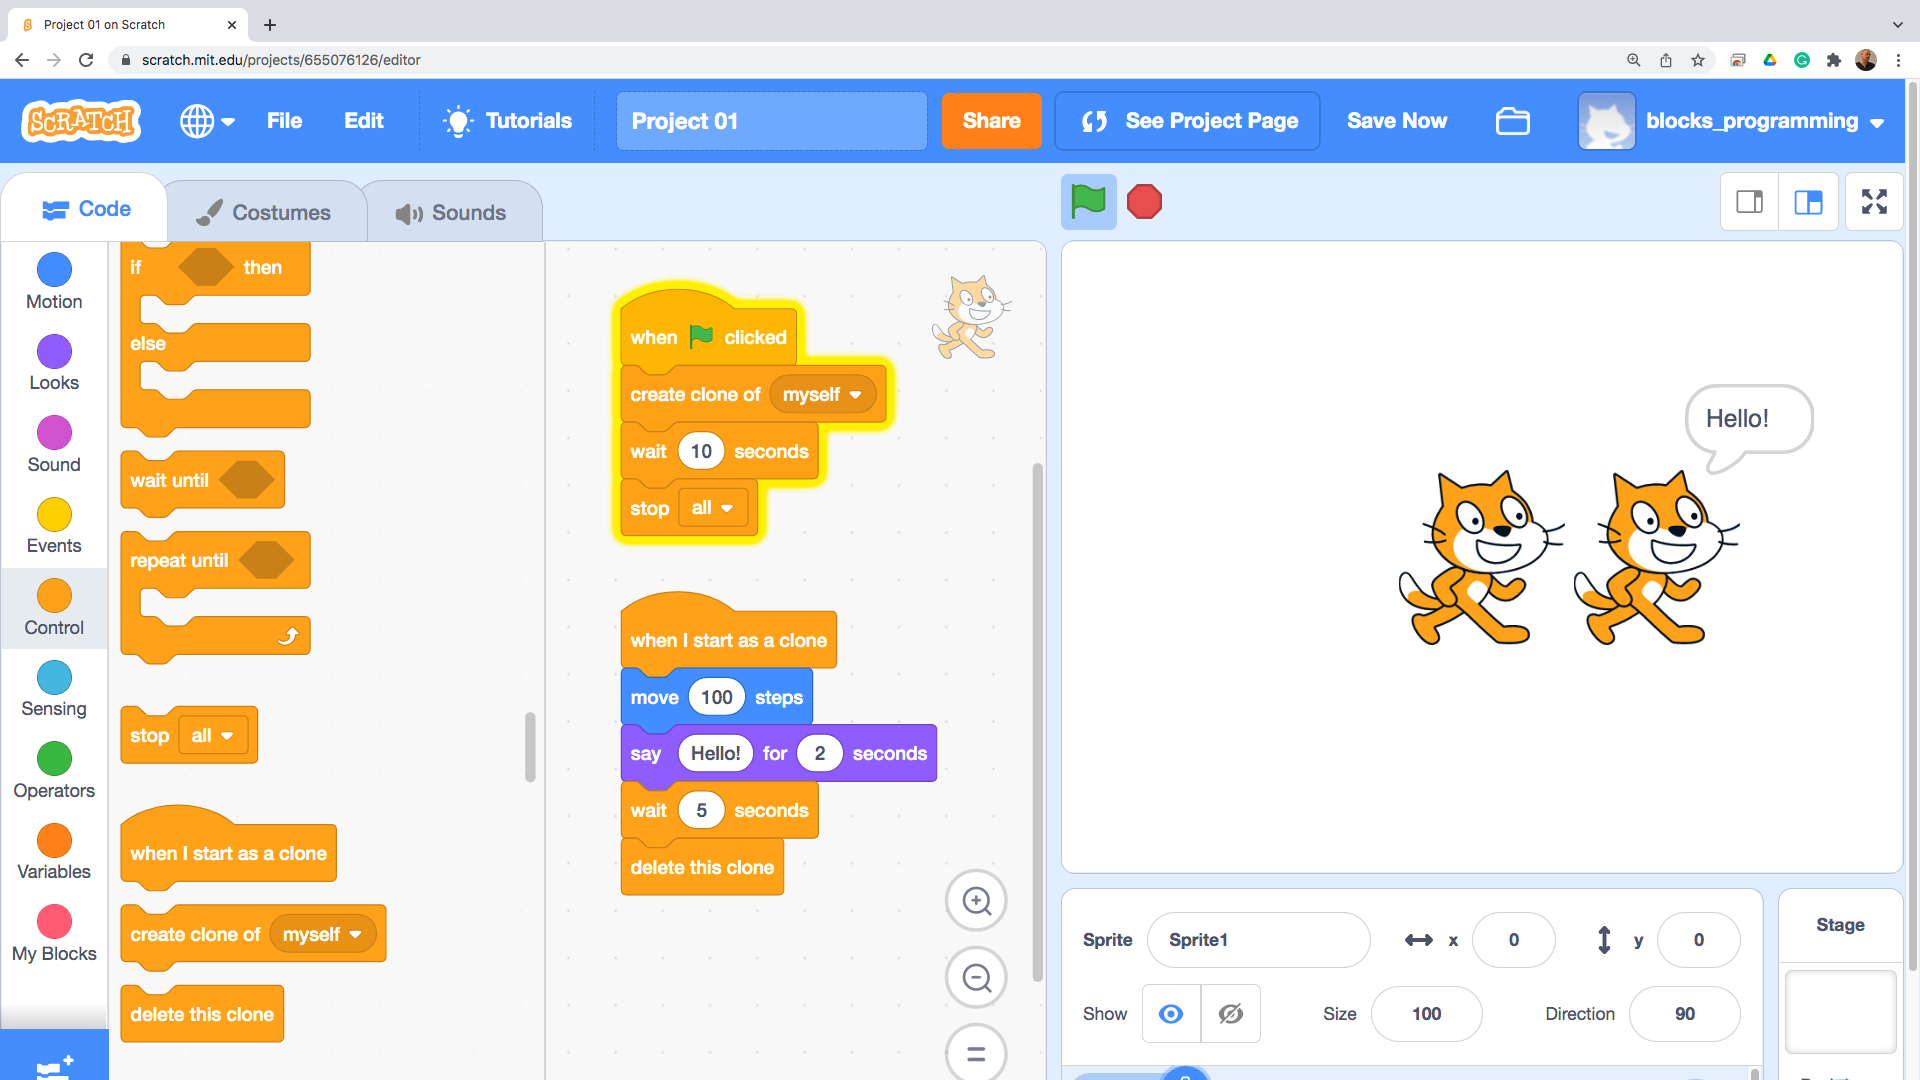
\includegraphics[width=1.0\linewidth,height=0.5\linewidth]{fig020040.png}
   \caption{Clone Sprites}
\label{fig020040}
\end{figure}

The light blue block group focuses on sprite interactions and includes a block designed to detect when a sprite touches a particular color (Fig. \ref{fig020041}). This block, represented by a hexagonal shape, is intended to be embedded within other blocks to create conditional behaviors based on color interactions.

To demonstrate the functionality of this block, a loop can be implemented. Within the loop, the kitten sprite will be moved to random coordinates, followed by a short pause before the next movement. The embedded color-touching block will trigger a condition when the kitten touches a specific color.

Incorporating this block into the loop allows you to create interactive scenarios where the program responds to specific color interactions. This can be particularly useful for implementing collision detection or triggering specific actions when the sprite encounters a particular color in the background or other sprites.

Experimenting with the color-touching block and combining it with other blocks and behaviors can add a new layer of interactivity to your projects. It allows you to create dynamic and responsive experiences where the sprite's actions are influenced by its interaction with colors in the scene.

Take advantage of the flexibility the color-touching block provides to enhance the engagement and immersion of your Scratch projects.

\begin{figure}[H]
   \centering
   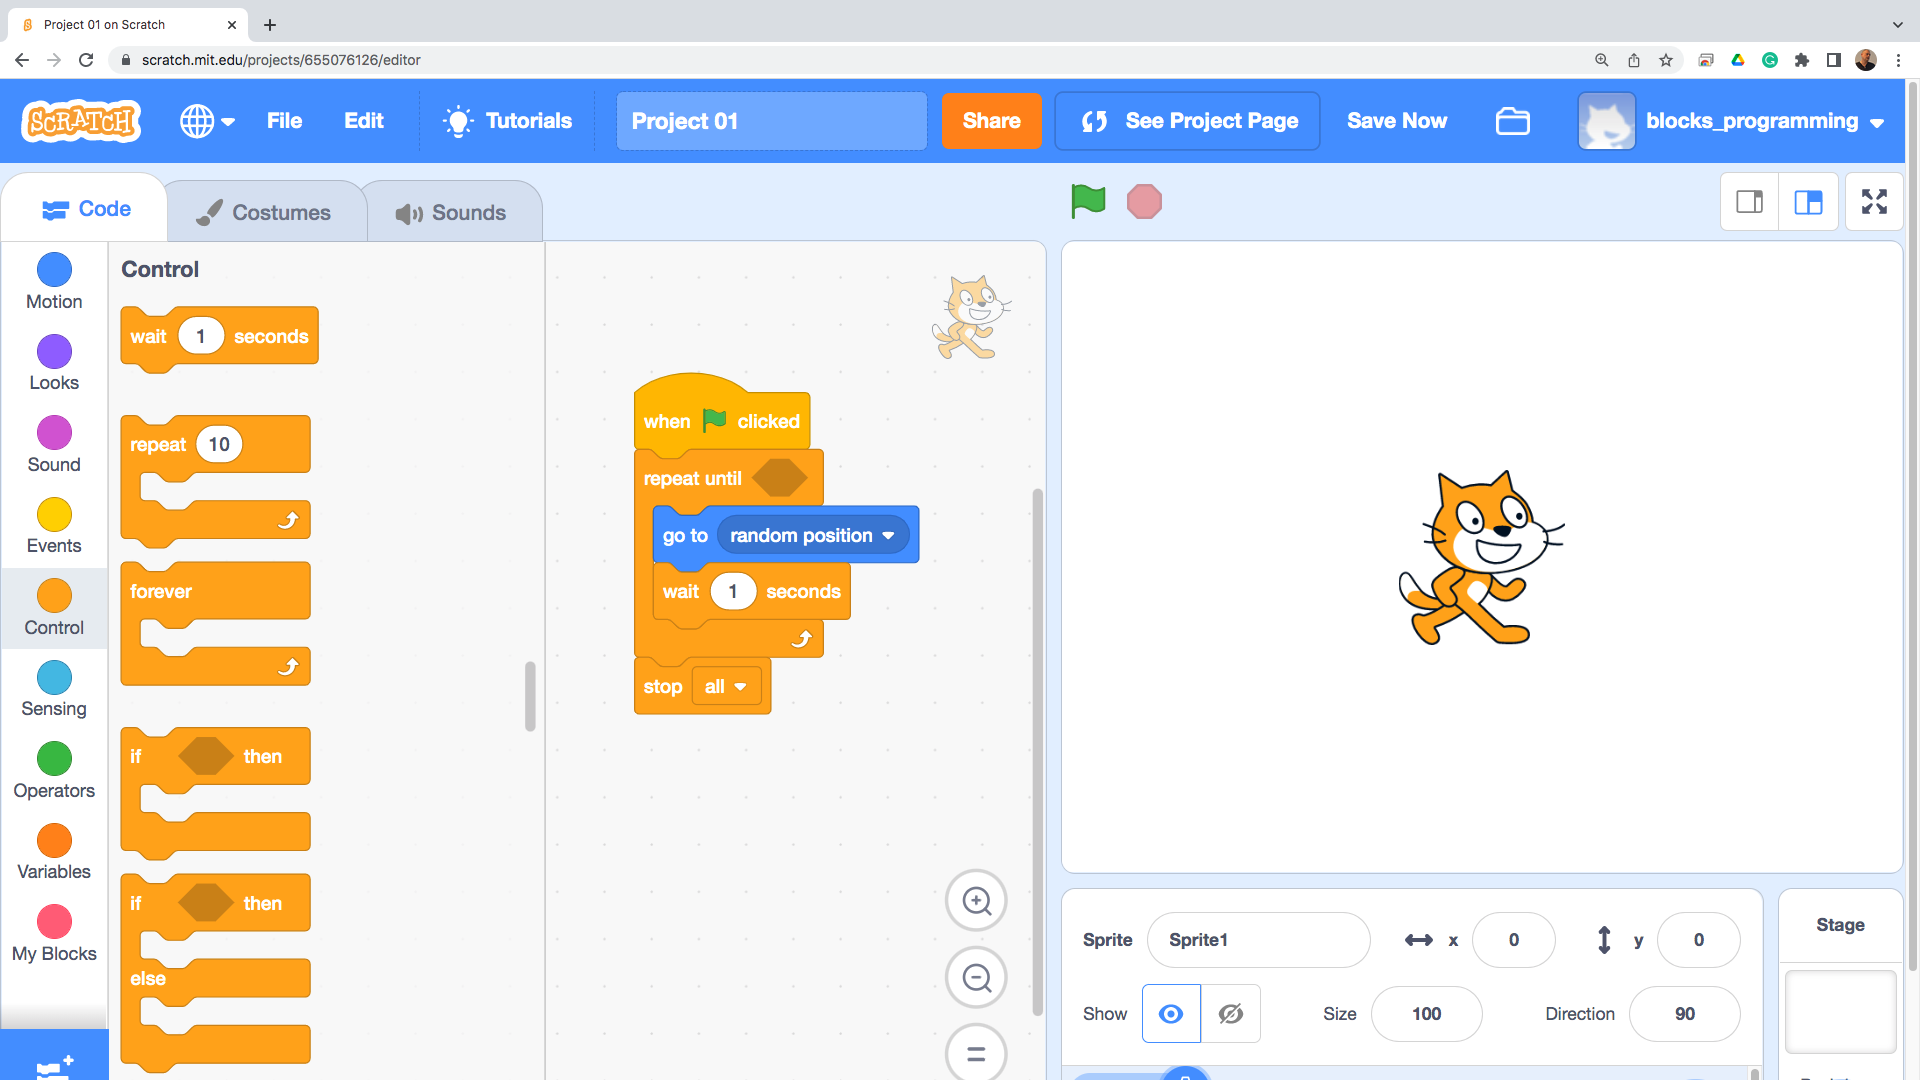
\includegraphics[width=1.0\linewidth,height=0.5\linewidth]{fig020041.png}
   \caption{Cyclical jump of random coordinates}
\label{fig020041}
\end{figure}

The current loop implementation lacks an end condition, resulting in an endless loop. To address this, we can incorporate the block that detects the touch of a specific color as the end condition. Let's introduce a new sprite, a red apple (Fig. \ref{fig020042}), which the kitten sprite will attempt to catch. Once the kitten successfully catches the apple, it will stop moving and emit a "meow" sound (Fig. \ref{fig020044}).

We can modify the loop structure to achieve this behavior by including the color-touching block as the loop's end condition. This block will check if the kitten touches the specific color associated with the apple sprite. The loop will terminate once the condition is met, and the subsequent instructions will be executed.

Introducing the red apple sprite and incorporating the color-touching block creates an interactive scenario where the kitten sprite actively pursues and catches the apple. This engagement adds a new level of gameplay to your Scratch project.

Remember to assign appropriate scripts to the apple sprite, such as changing its position randomly to provide an ongoing challenge for the kitten sprite. Additionally, don't forget to include the sound block to emit the "meow" sound when the kitten successfully catches the apple, enhancing the audiovisual experience of your project.

Utilize the various blocks and sprites to create dynamic and engaging interactions in your Scratch projects, allowing users to immerse themselves in captivating scenarios.

\begin{figure}[H]
   \centering
   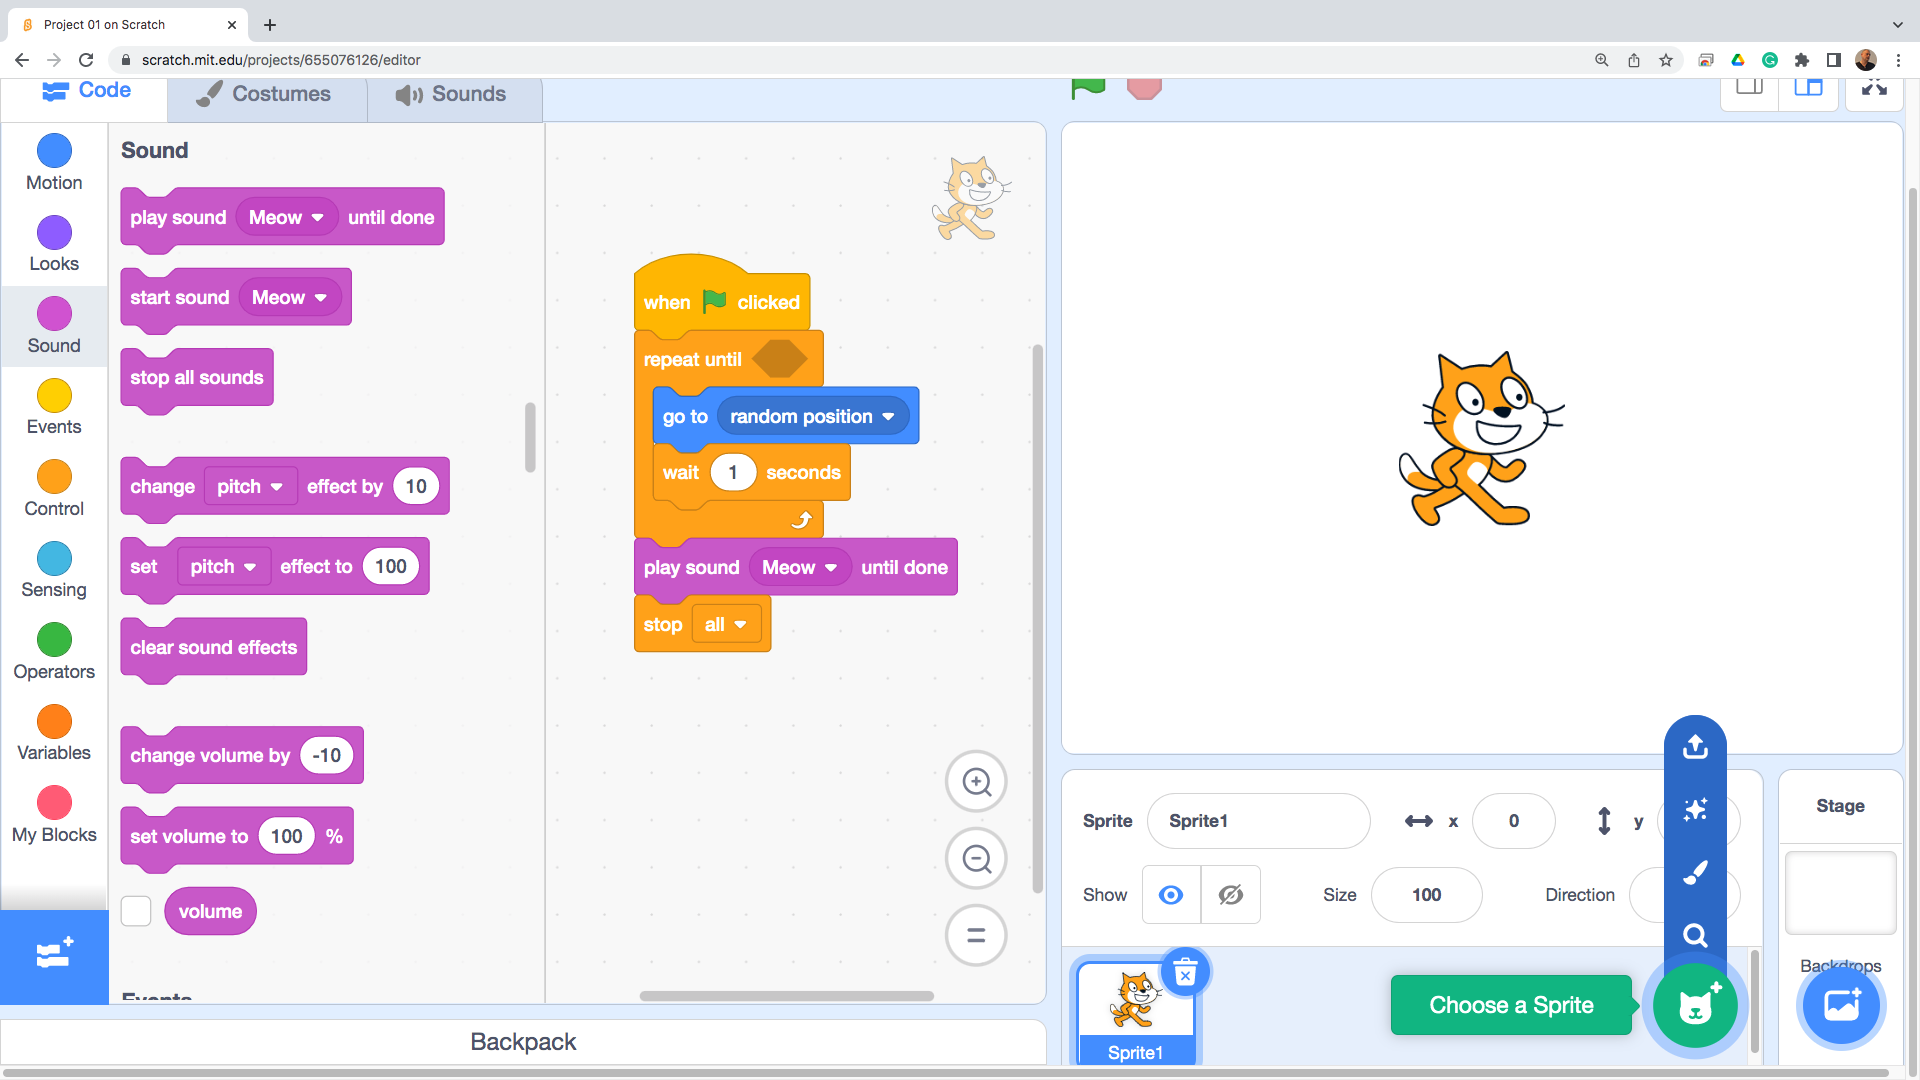
\includegraphics[width=1.0\linewidth,height=0.5\linewidth]{fig020042.png}
   \caption{Add sprite}
\label{fig020042}
\end{figure}

\begin{figure}[H]
   \centering
   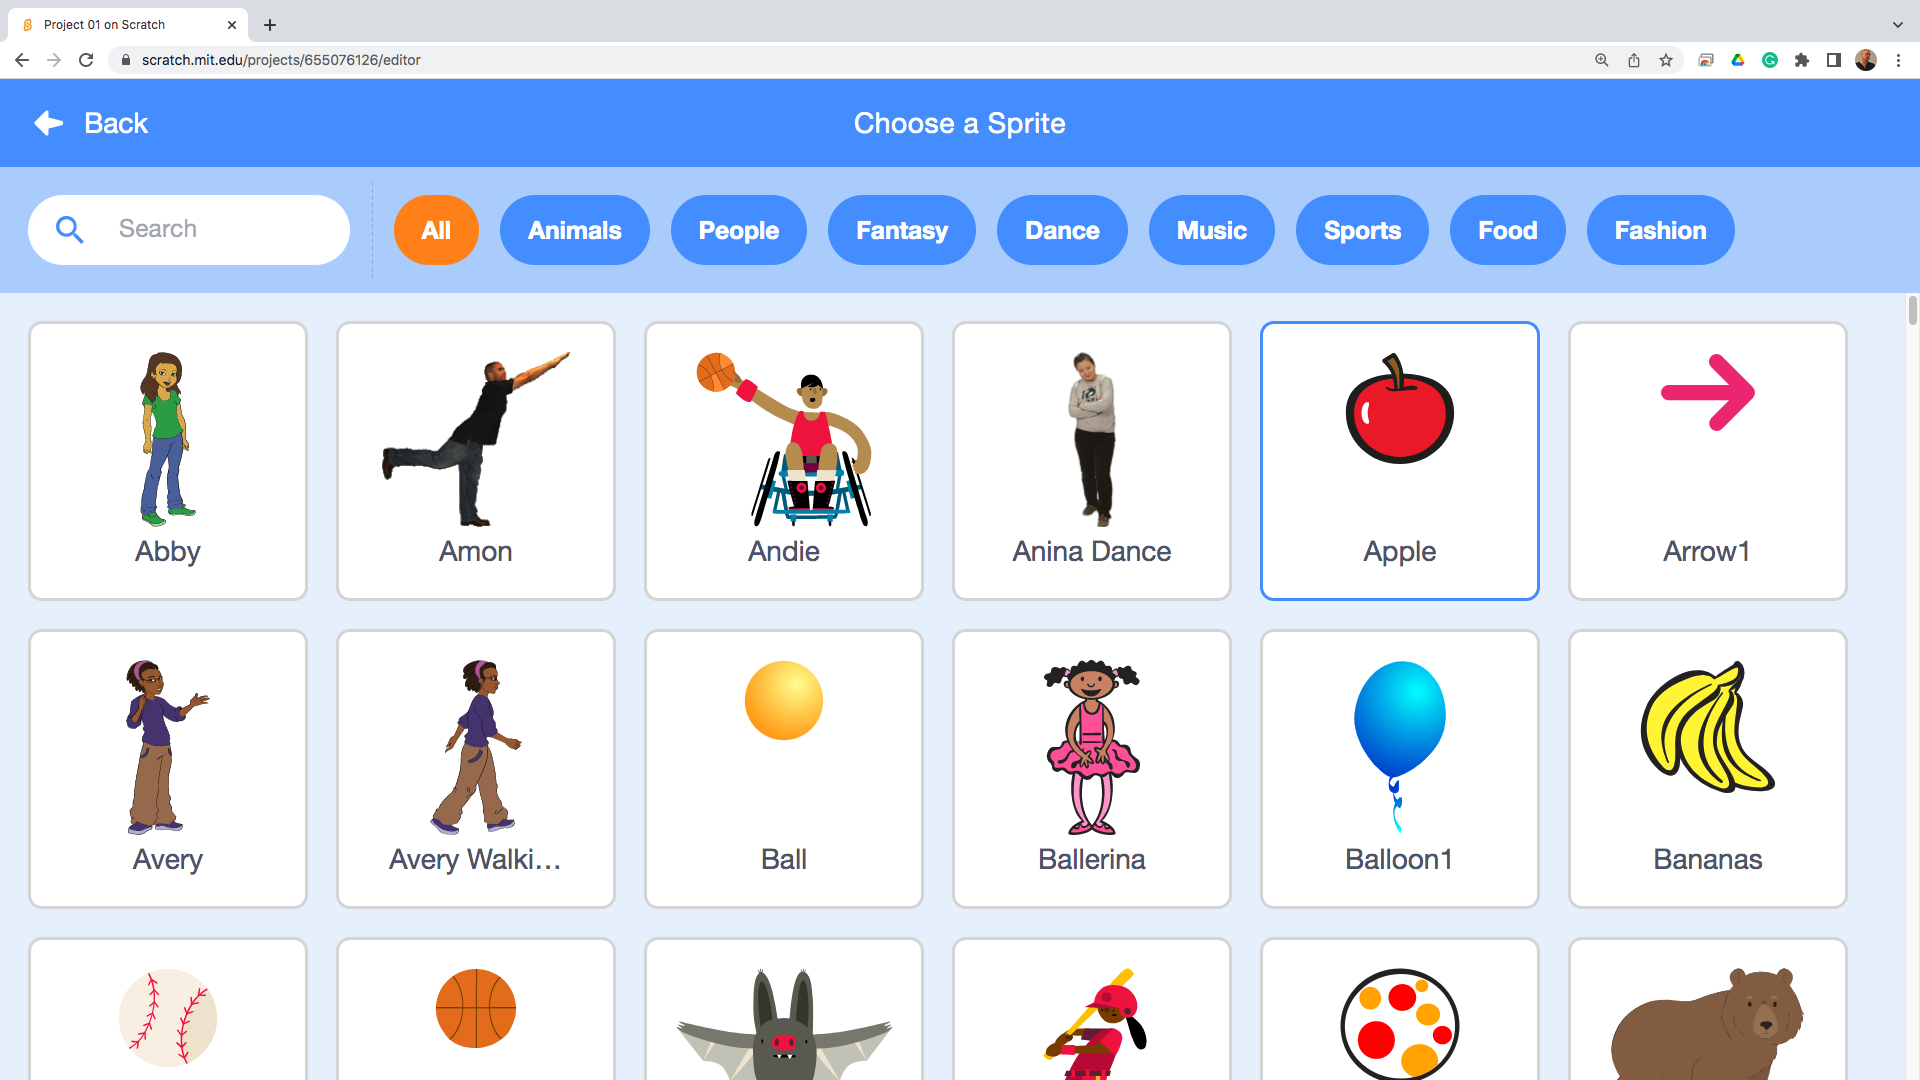
\includegraphics[width=1.0\linewidth,height=0.5\linewidth]{fig020043.png}
   \caption{Choose sprite from gallery}
\label{fig020043}
\end{figure}

\begin{figure}[H]
   \centering
   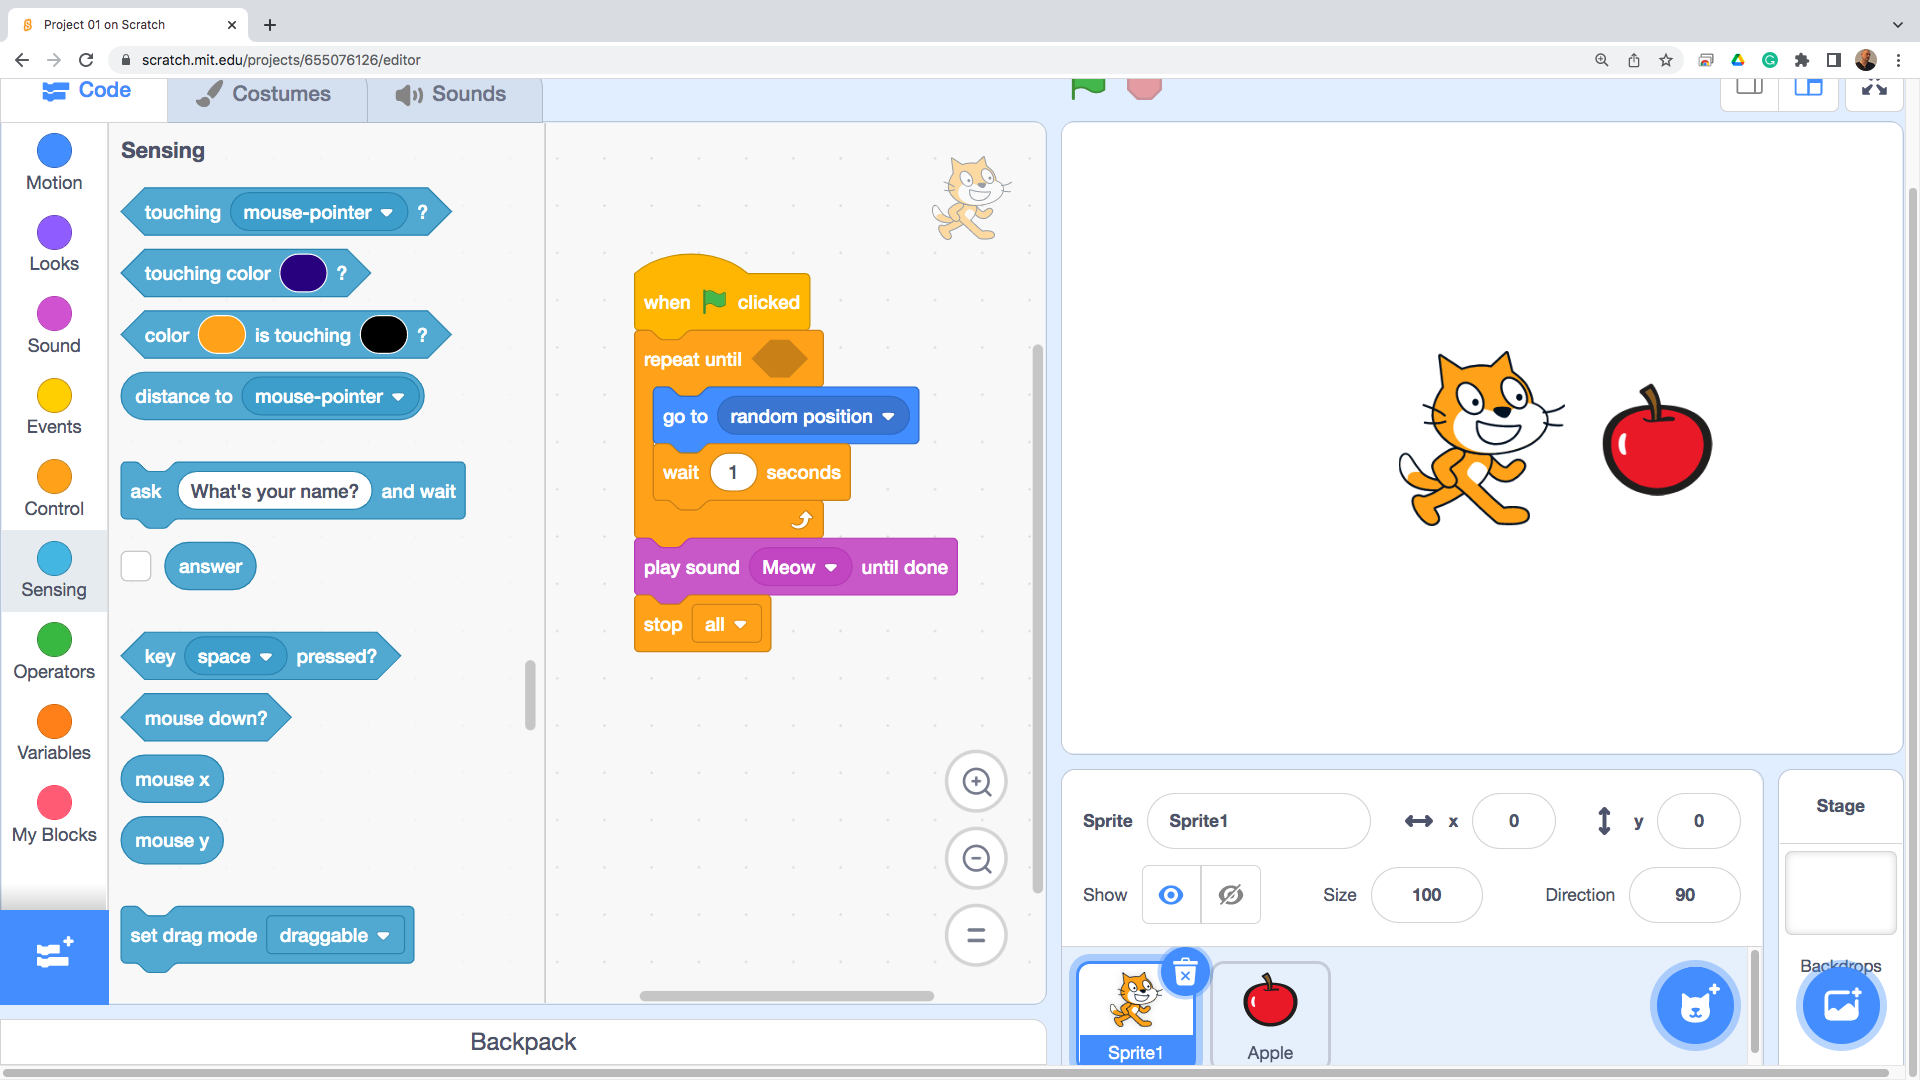
\includegraphics[width=1.0\linewidth,height=0.5\linewidth]{fig020044.png}
   \caption{Positioning the apple}
\label{fig020044}
\end{figure}

When working with sprites, one common challenge is detecting whether two sprites touch or overlap. Several techniques can be used to identify collisions, but one particularly effective method is based on detecting specific colors. Modern computers can display over 16 million colors, providing ample opportunities to leverage color detection for collision detection.

In our scenario, since the apple sprite is red, we can use the touching of the red color as the condition to end the loop. We can determine if it has successfully caught the apple by detecting when the kitten sprite touches the red color (Fig. \ref{fig020045}).

This approach offers limitless possibilities for detecting collisions by carefully selecting the colors associated with the sprites. It allows for precise and reliable collision detection, enhancing the interactive nature of your Scratch project.

By implementing the color-touching block with the red color, you ensure that the loop terminates when the kitten catches the apple. You can further extend this concept by exploring different color combinations and their corresponding actions or events in your project.

Adjust the sprite positions, add appropriate scripts, and provide visual and auditory feedback to enhance the user experience and engagement with your project.

\begin{figure}[H]
   \centering
   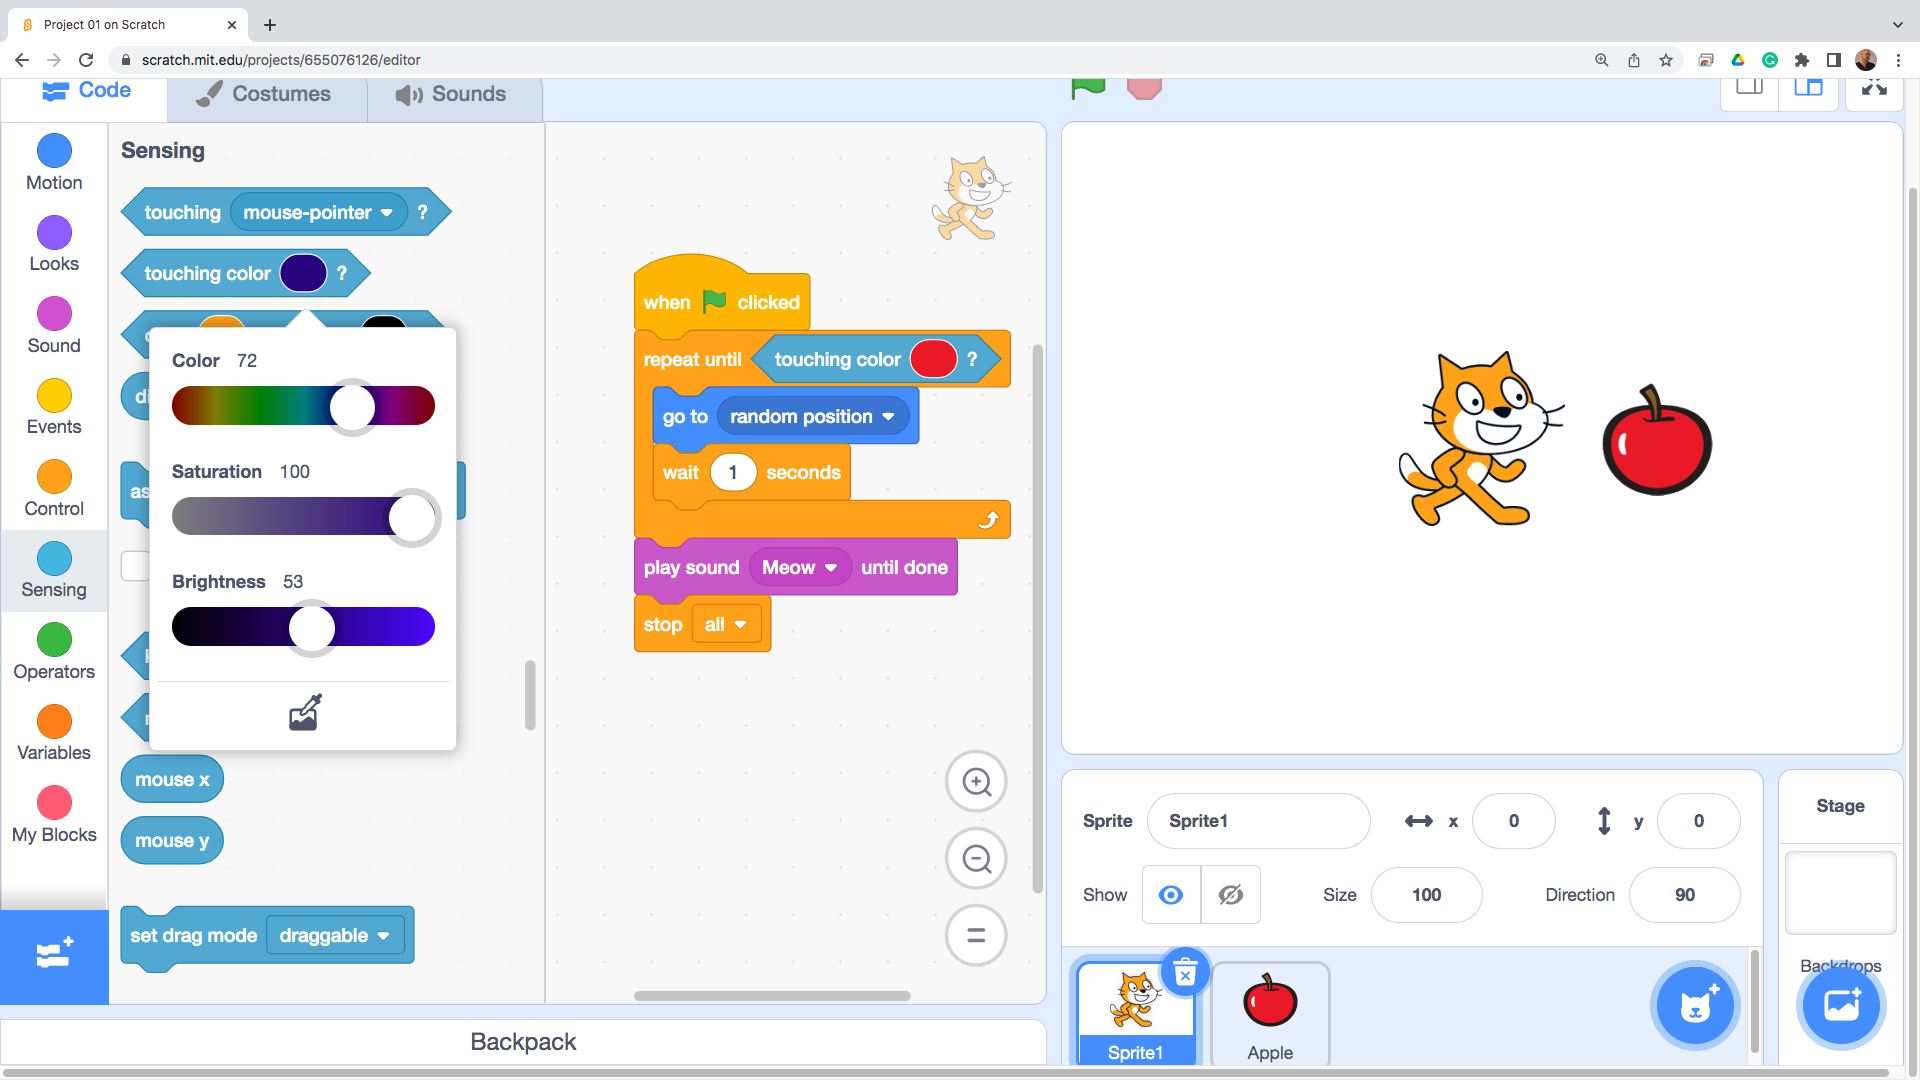
\includegraphics[width=1.0\linewidth,height=0.5\linewidth]{fig020045.png}
   \caption{Touch by color}
\label{fig020045}
\end{figure}

The previous block detected a collision between the kitten and the apple based on any part of the kitten touching the apple's red color. However, for more precise collision detection, we can focus on checking the kitten's black outline against the apple's red color. This level of detail can be achieved using the following block specifically designed for this purpose (Fig. \ref{fig020046}).

By utilizing this block, you can ensure that the collision is detected only when the black outline of the kitten touches the red color of the apple, providing a more accurate representation of the interaction between the sprites.

Implementing this block allows for finer control over collision detection, enhancing your project's visual and functional aspects. It provides a more realistic simulation of sprite interactions, ensuring the collision is triggered only when the specific criteria are met.

Remember to adjust the positions of the sprites, incorporate appropriate scripts, and provide visual and audio cues to provide a seamless and engaging user experience.

\begin{figure}[H]
   \centering
   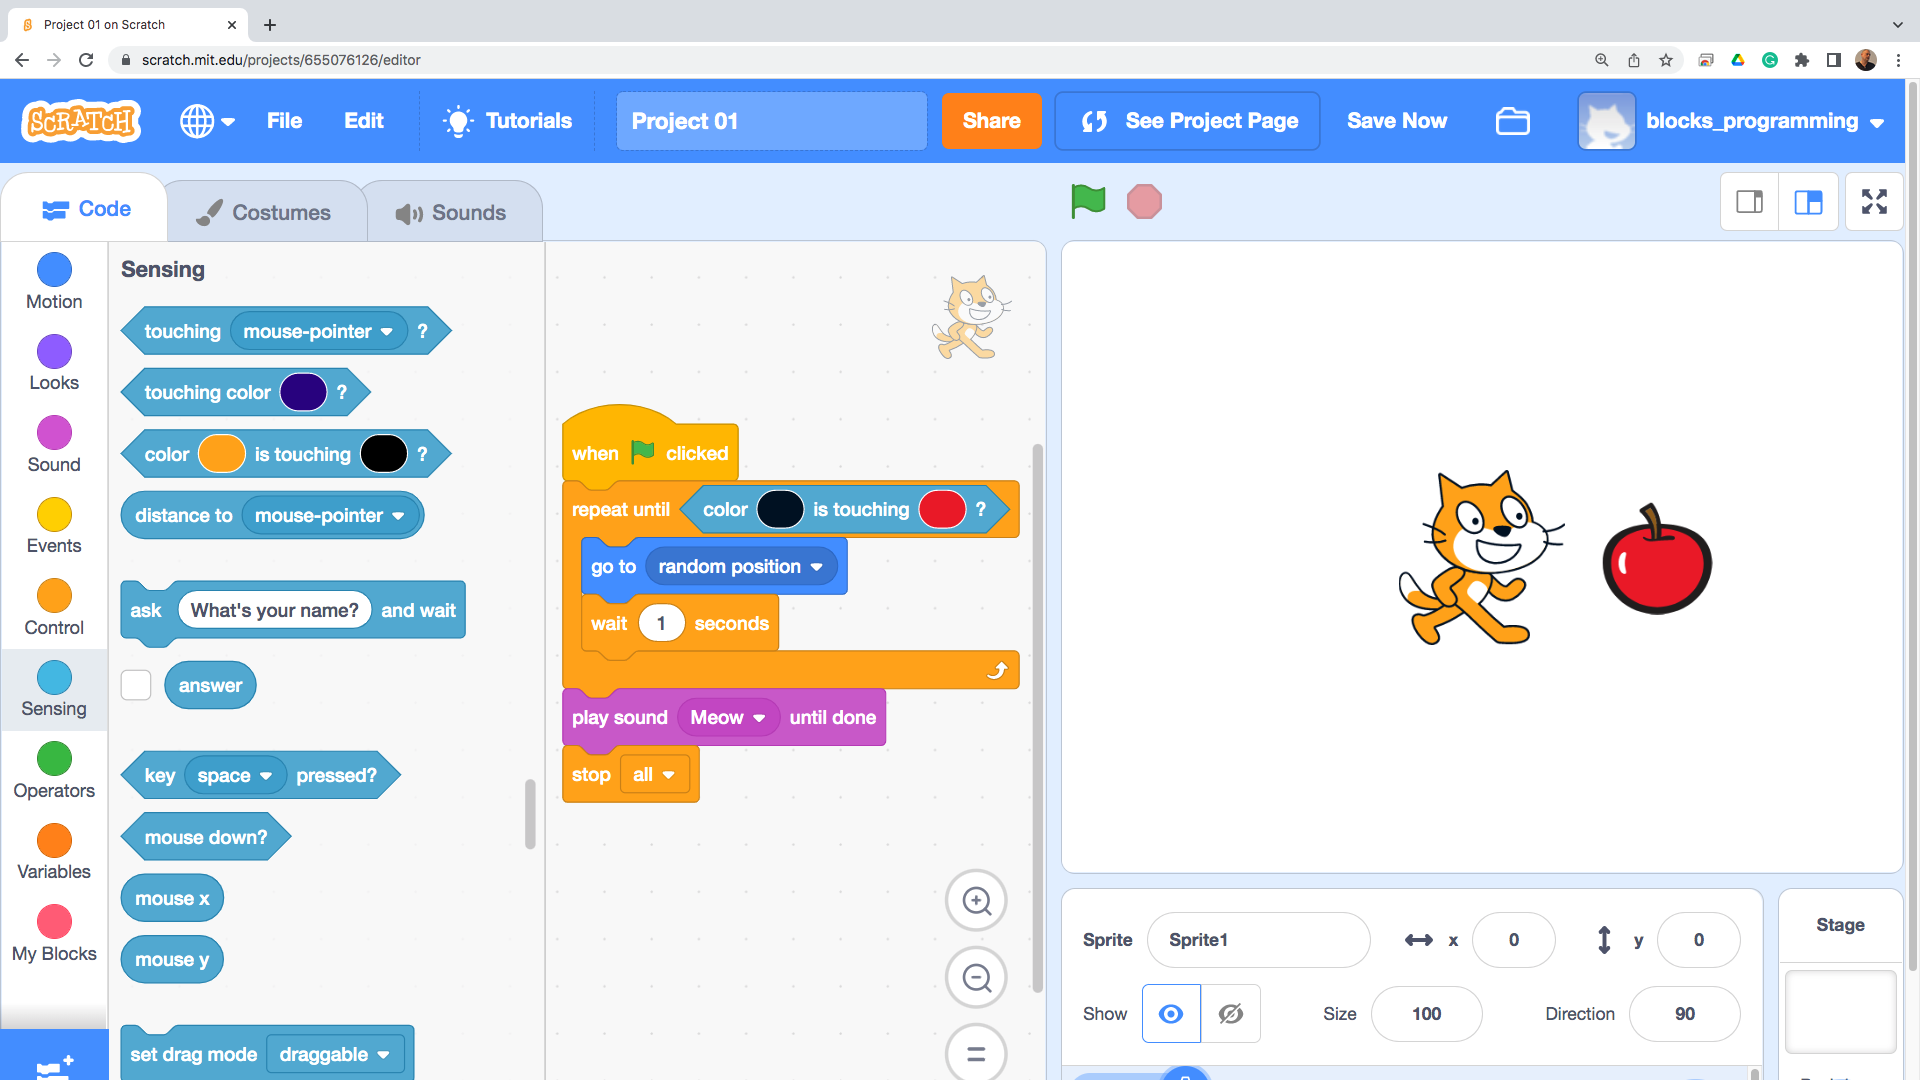
\includegraphics[width=1.0\linewidth,height=0.5\linewidth]{fig020046.png}
   \caption{Collision on two preset colors}
\label{fig020046}
\end{figure}

With its oval shape, the next block provides the program with the distance between the sprite and the mouse pointer. This block is designed to be embedded within one of the arithmetic expression blocks, as indicated by its oval shape (Fig. \ref{fig020047}).

This block allows you to dynamically calculate the distance between the sprite and the mouse pointer, allowing for interactive behaviors and responsive animations. This distance information can be used in various ways, such as adjusting the sprite's movement speed based on proximity to the mouse or triggering specific actions when the sprite is within a certain distance from the mouse pointer.

Integrating this block within arithmetic expressions empowers you to create more complex and dynamic calculations involving the sprite's position and the mouse pointer. This enhances the interactivity of your project and enables more sophisticated interactions between the sprite and user input.

Remember to combine this block with other relevant blocks and scripts to achieve the desired behavior in your project. Experiment with different scenarios and leverage the flexibility of Scratch to create engaging experiences for your users.

\begin{figure}[H]
   \centering
   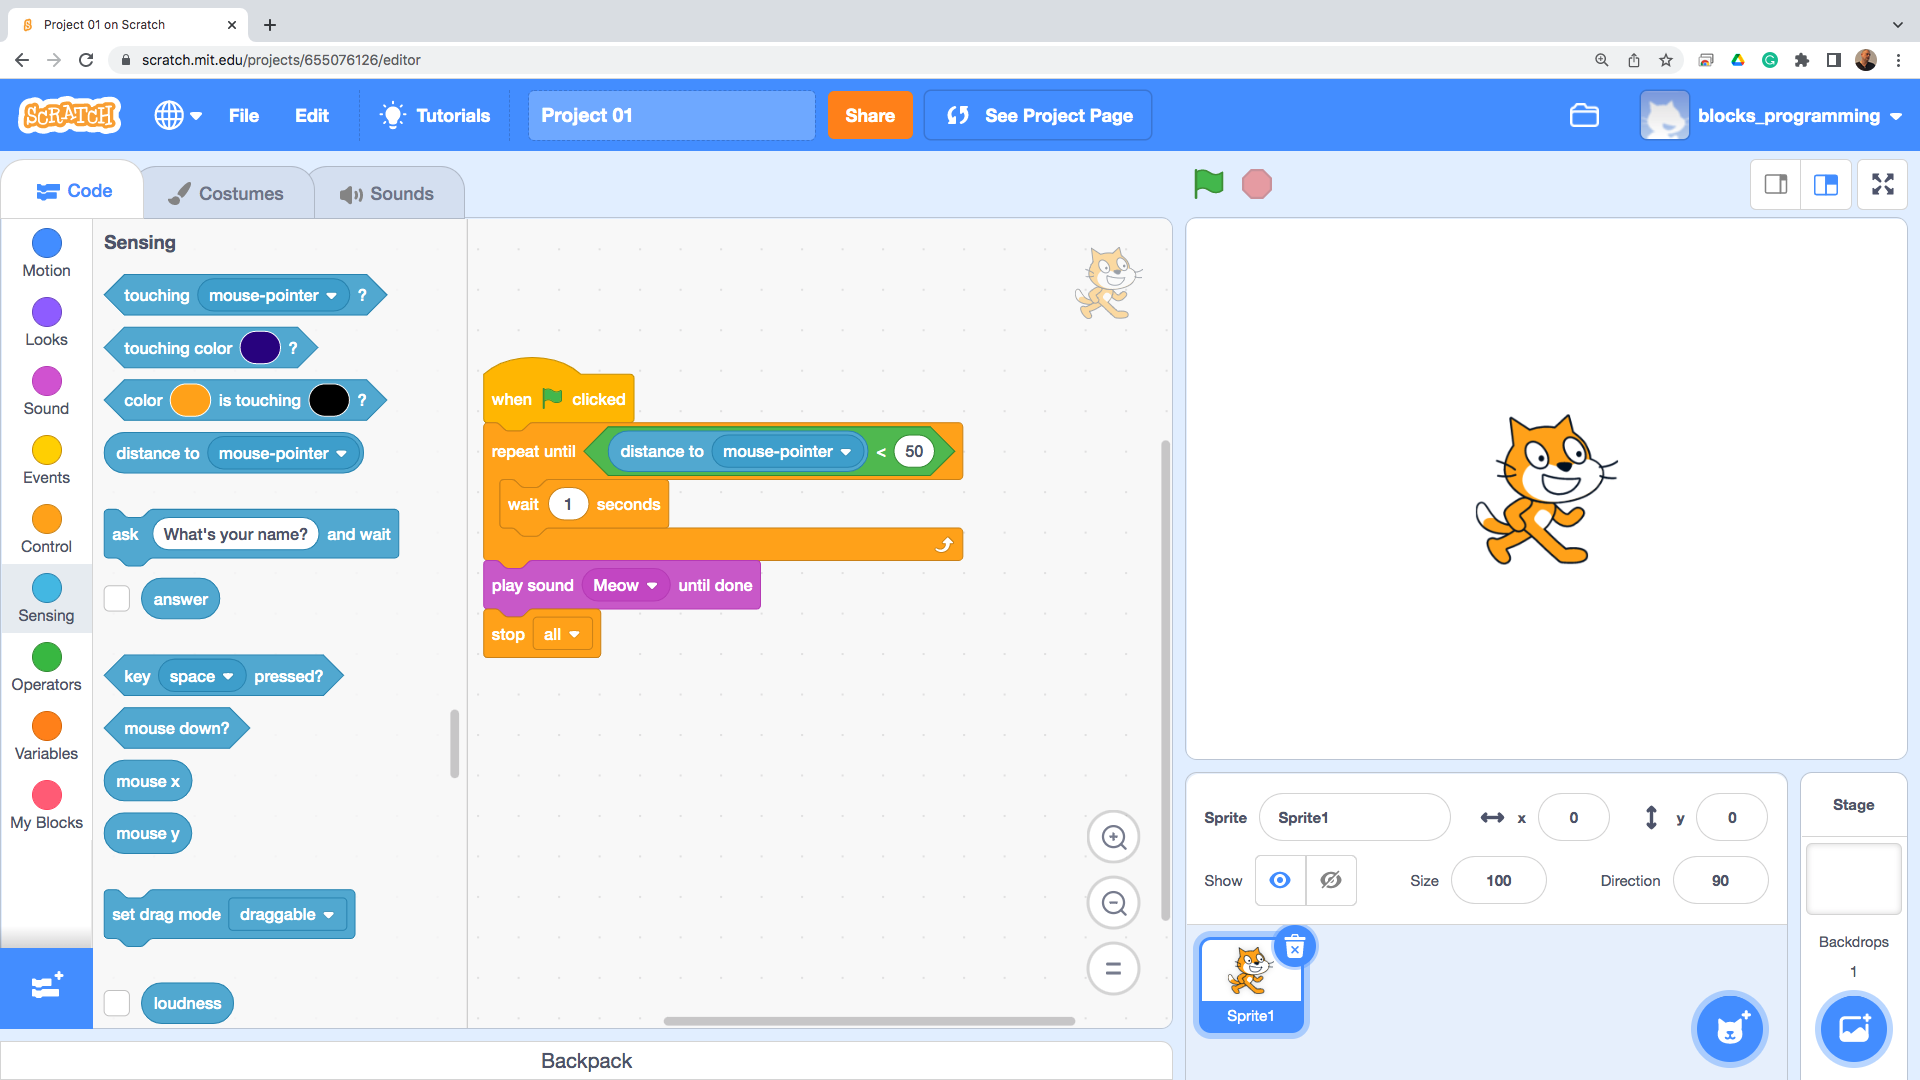
\includegraphics[width=1.0\linewidth,height=0.5\linewidth]{fig020047.png}
   \caption{Mouse Pointer Distance}
\label{fig020047}
\end{figure}

To enable user input through typing, the next block in the light blue group comes into play (Fig. \ref{fig020048}). This block allows the animated character to prompt the user by displaying specific text, indicating what is expected to be typed.

With this block, you can create interactive experiences where the user is prompted to enter information or provide responses. Whether answering a question, filling in a form, or engaging in a dialogue with the character, this block opens up user interaction and dynamic storytelling possibilities.

You can guide the user on desired input by customizing the text in the prompt. This can be particularly helpful for creating educational activities, quizzes, or interactive narratives where user input plays a central role.

Remember to combine this block with other blocks that capture and process user input to create meaningful interactions within your project. You can store the user's input in variables, validate the input, and trigger specific actions based on the typed response.

Utilize this block to empower users to actively participate and engage with your project by typing in their input and influencing the behavior of the animated character.

\begin{figure}[H]
   \centering
   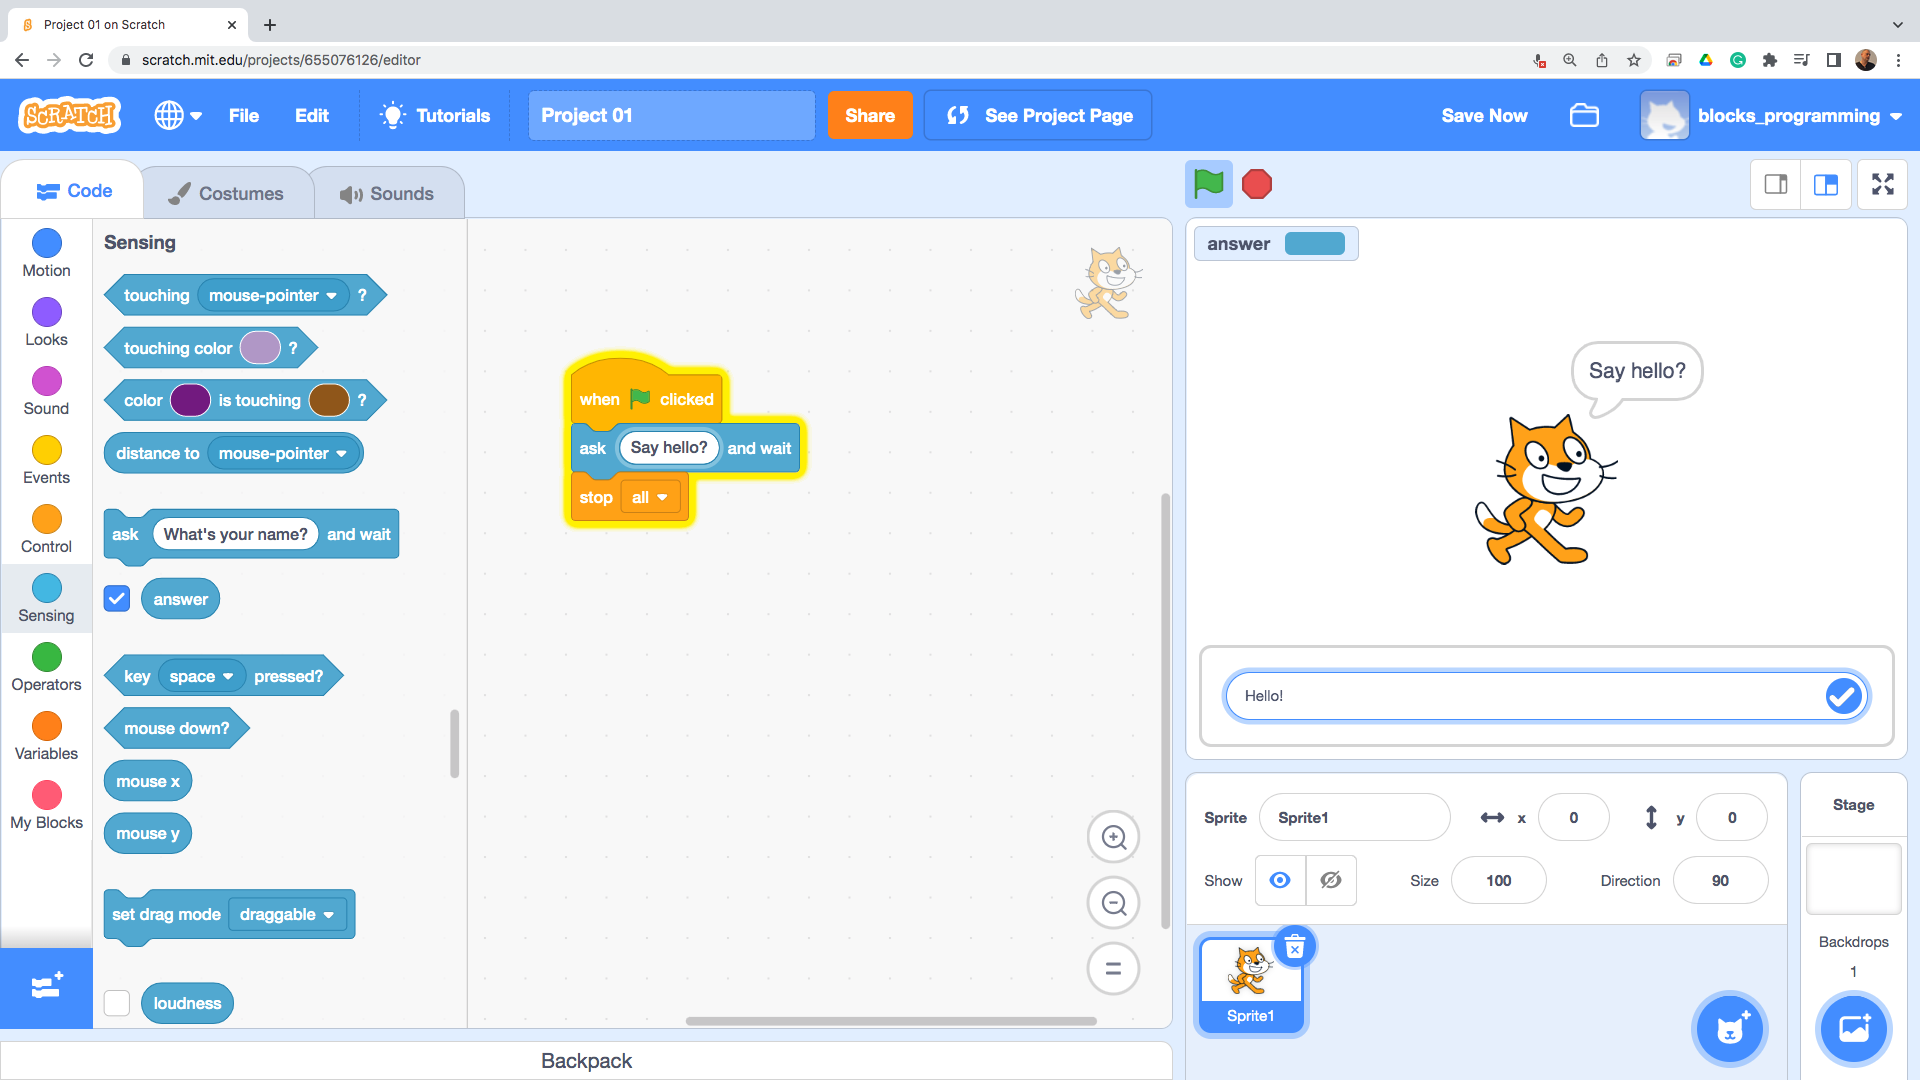
\includegraphics[width=1.0\linewidth,height=0.5\linewidth]{fig020048.png}
   \caption{Enter text}
\label{fig020048}
\end{figure}

The next block is one of the hexagonal blocks designed for embedding. Its purpose is to determine whether a specific key has been pressed, and it returns a result of "true" in such cases (Fig. \ref{fig020049}).

Using this block, you can create interactive experiences where the program responds to specific key inputs from the user. This opens up possibilities for implementing keyboard-controlled games, interactive simulations, or any scenario where user input through key presses is crucial.

You can embed this block within conditional statements to trigger specific actions based on the key pressed. For example, you can make a character jump when the spacebar is pressed, move in different directions using arrow keys, or even simulate typing effects by capturing and displaying typed characters on the screen.

This block adds a layer of interactivity to your project, allowing users to engage and control the behavior of the animated character or influence the program's flow through keyboard input.

Remember to provide clear instructions or prompts to inform users about the keys they can press to interact with your project. Consider handling multiple key presses simultaneously or implementing key combinations for more complex interactions.

With this block, you can create dynamic and engaging experiences that respond to user input through key presses, making your project more interactive and immersive.

\begin{figure}[H]
   \centering
   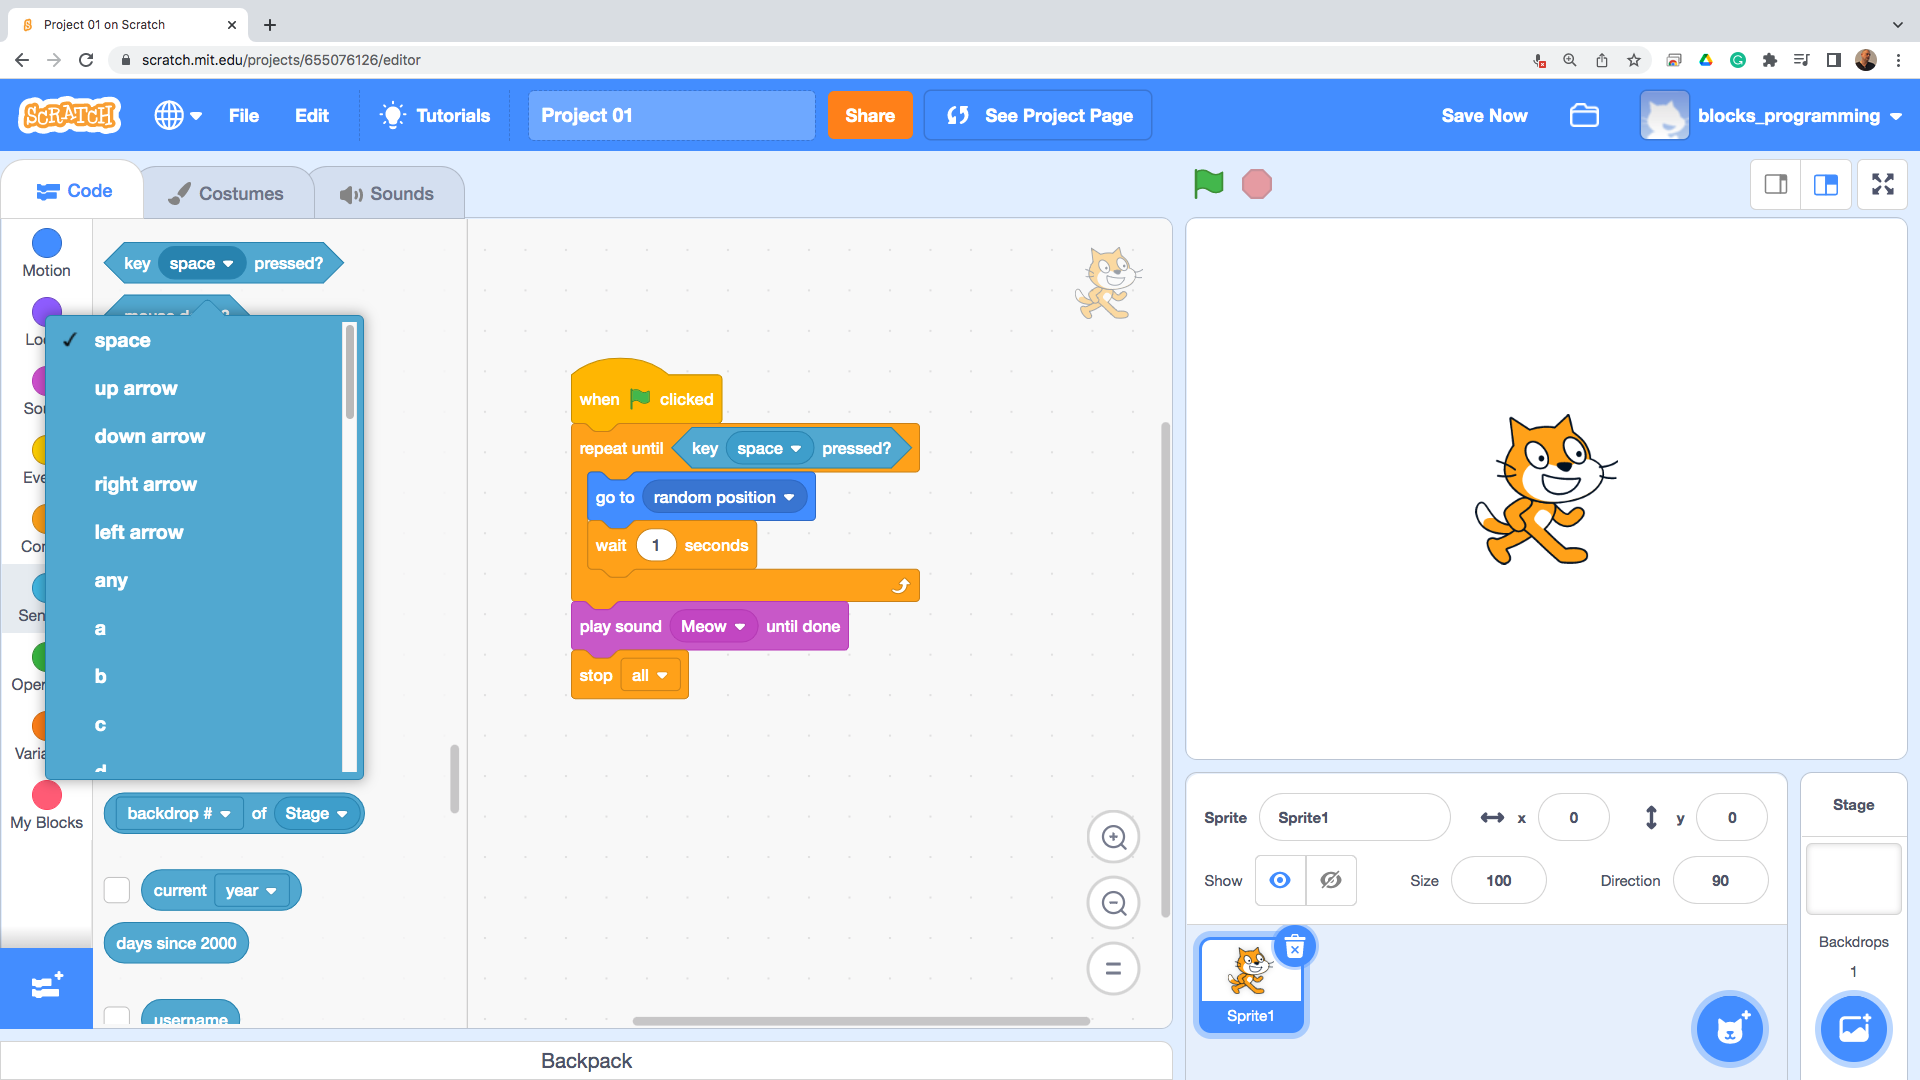
\includegraphics[width=1.0\linewidth,height=0.5\linewidth]{fig020049.png}
   \caption{Defining key pressed}
\label{fig020049}
\end{figure}

Similar behavior can be achieved with the next block, which allows you to detect mouse clicks instead of key presses (Fig. \ref{fig020050}).

This hexagonal block is specifically designed for embedding and returns a result of "true" when a mouse button is clicked. Using this block, you can create interactive experiences where the program responds to mouse clicks from the user.

With this block, you can implement various functionalities based on mouse interactions. For example, you can create clickable buttons, interactive menus, drag-and-drop interactions, or any scenario where user input through mouse clicks is essential.

To utilize this block effectively, you can embed it within conditional statements to trigger specific actions when clicking the mouse button. This allows you to create interactive elements that respond to user interactions in real time.

Consider providing visual feedback to users when they click the mouse button, such as changing the appearance of a button or triggering animations. This enhances the user experience and indicates that their interaction has been registered.

Combining this block with other blocks and programming concepts allows you to create engaging projects that respond to user input through mouse clicks. Whether you're designing games, simulations, or interactive applications, this block opens up a wide range of possibilities for user interaction and engagement.

Remember to consider the context in which the mouse click is expected and provide appropriate instructions or visual cues to guide users on interacting with your project.

Utilize the power of this block to make your project more interactive, intuitive, and enjoyable for users interacting with it through mouse clicks.

\begin{figure}[H]
   \centering
   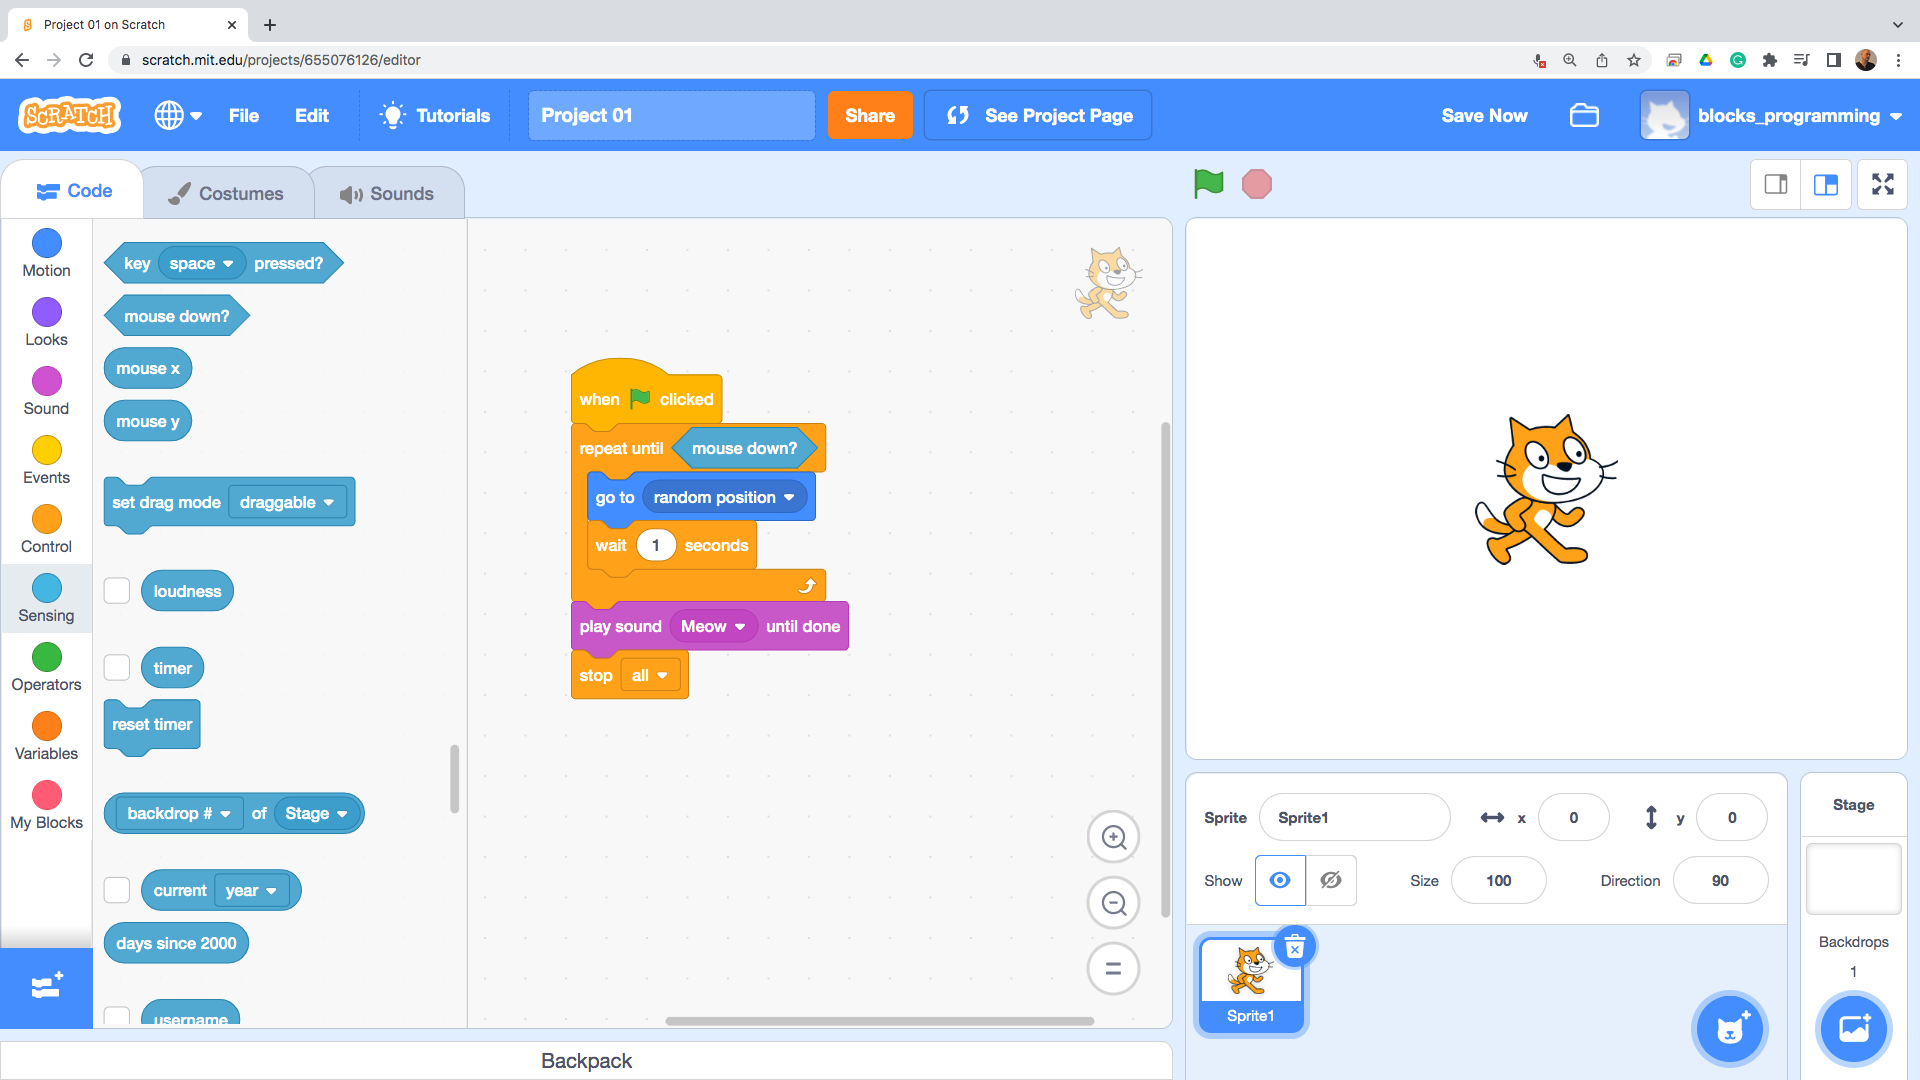
\includegraphics[width=1.0\linewidth,height=0.5\linewidth]{fig020050.png}
   \caption{Detect mouse button pressed}
\label{fig020050}
\end{figure}

The following two blocks are oval-shaped and are designed to be embedded in your program. The first block provides the coordinates of the animated character along the x-axis, while the second block gives the coordinates along the y-axis (Fig. \ref{fig020051}).

Using these blocks, you can access the precise position of the animated character within the program's coordinate system. This information can be valuable for implementing various functionalities and interactions within your project.

The block that provides the x-coordinate allows you to retrieve the horizontal position of the animated character. This can be useful for tasks such as controlling the character's movement along a specific path, aligning objects or sprites relative to the character's position, or triggering actions based on its location within the scene.

Similarly, the block that provides the y-coordinate gives you access to the vertical position of the animated character. This can be utilized for tasks such as controlling vertical movement, determining collision detection with other objects, or dynamically positioning elements based on the character's position.

You can create dynamic and responsive behaviors based on the animated character's coordinates by embedding these blocks within your program's logic. This allows you to build projects that adapt and react to changes in position, enabling immersive experiences for your users.

Consider using these coordinate blocks and other blocks and programming concepts to create more complex behaviors and interactions. By combining them with conditionals, loops, and other mathematical operations, you can achieve precise control and coordination within your project.

Remember to consider the coordinate system used by the programming environment and ensure you understand how the values are interpreted and displayed. This will help you accurately position and control your animated character within the project.

Harness the power of these coordinate blocks to bring your animated character to life and create dynamic, interactive experiences in your Scratch projects.

\begin{figure}[H]
   \centering
   \includegraphics[width=1.0\linewidth,height=0.5\linewidth]{fig020051.png}
   \caption{Coordinates of the animated character}
\label{fig020051}
\end{figure}

During program execution, a timer continuously runs, measuring the elapsed time since the program's start. You can use the following block to reset this timer and start counting from zero again (Fig. \ref{fig020052}).

The block that resets the timer allows you to precisely control and track the passage of time within your program. By resetting the timer at specific points in your code, you can accurately measure the duration of certain events or actions, implement time-based behaviors, or create time-sensitive functionalities.

When you use the reset timer block, the timer will start counting from zero as soon as the block is executed. Any subsequent time-based calculations or comparisons you perform will be based on the time elapsed since the reset.

Consider incorporating the reset timer block into your program when measuring intervals, setting time-based conditions, or synchronizing actions based on specific time thresholds. This block can be handy for implementing time-based animations, timed challenges, or creating time-limited interactions.

Remember to combine the reset timer block with other programming constructs, such as conditionals, loops, or event triggers, to create dynamic and responsive behaviors based on time measurements.

Utilize the power of the reset timer block to accurately track and manage time within your Scratch projects, enhancing the user experience and enabling a wide range of time-based functionalities.

\begin{figure}[H]
   \centering
   \includegraphics[width=1.0\linewidth,height=0.5\linewidth]{fig020052.png}
   \caption{Reset Timer}
\label{fig020052}
\end{figure}

The next block in the Scratch programming interface is an oval-shaped block that serves a versatile purpose. It allows you to access and retrieve various information within your program, such as background information, variables, or sound levels (Fig. \ref{fig020053}).

By using this block, you can gather essential data that can be utilized for decision-making, conditional statements, or displaying relevant information to the user. The specific information you retrieve depends on the context in which you use the block.

For example, if you want background information, this block can provide details about the current background image or its properties. You can use this information to dynamically adapt your program's behavior based on the displayed background.

Similarly, when working with variables, the oval block lets you retrieve the current value stored in a variable. This enables you to utilize the variable's value in calculations, comparisons, or displaying it to the user.

Additionally, if you're working with sound, this block allows you to access the sound level, providing information about the current sound's volume or intensity. You can utilize this information to adjust the behavior of your program based on the sound level.

By leveraging the power of the oval-shaped block, you can access important data within your program, enabling dynamic and context-aware functionality. Explore the various possibilities and incorporate this block into your code to enhance interactivity, responsiveness, and user engagement in your Scratch projects.

\begin{figure}[H]
   \centering
   \includegraphics[width=1.0\linewidth,height=0.5\linewidth]{fig020053.png}
   \caption{Scene Component Information}
\label{fig020053}
\end{figure}

The final block in this group is another embedded block that provides unique functionality. It returns the number of days that have passed since the year 2000, often referred to as the "days since 2000" value (Fig. \ref{fig020054}).

This block allows you to calculate the precise number of days that have elapsed since the beginning of 2000. It is helpful when working with time-related calculations or creating dynamic time-based functionalities in your Scratch projects.

Using this block, you can keep track of the passage of time within your program, create timers, implement countdowns, or even trigger events based on specific dates or durations. It gives you a reliable way to work with dates and times in your Scratch projects, adding a new dimension of interactivity and functionality.

Whether you want to create a game with time-based challenges, simulate real-time events, or display the current day count, this block provides the necessary information to achieve your desired outcomes.

Experiment with this block, combine it with other blocks and explore the possibilities of time-based programming in Scratch. Let your imagination soar as you leverage the "days since 2000" block to create engaging and dynamic user experiences.

\begin{figure}[H]
   \centering
   \includegraphics[width=1.0\linewidth,height=0.5\linewidth]{fig020054.png}
   \caption{Number of days since the beginning of the century}
\label{fig020054}
\end{figure}

The green block group consists of four oval-shaped blocks for performing arithmetic operations: addition, subtraction, multiplication, and division (Fig. \ref{fig020055}).

These blocks enable you to manipulate numerical values within your Scratch projects, allowing you to perform calculations and create dynamic behaviors. Whether you need to compute scores, keep track of variables, or implement complex mathematical algorithms, these arithmetic blocks provide the foundation for your mathematical operations.

The addition block (+) allows you to add two or more numbers, combining their values into a single sum. The subtraction block (-) lets you subtract one number from another, determining the difference between them. The multiplication block (×) enables you to multiply two or more numbers, generating the product of their values. Lastly, the division block (÷) allows you to divide one number by another, providing the quotient or result of the division.

Using these arithmetic blocks, you can create interactive calculations, control the behavior of sprites, or implement game mechanics that rely on mathematical operations. They provide you with the flexibility to perform a wide range of numerical computations, enhancing the functionality and interactivity of your Scratch projects.

Feel free to experiment with these blocks, combine them with other elements, and explore the possibilities of mathematical programming in Scratch. Whether you're working on educational projects, games, or simulations, the arithmetic blocks empower you to bring your ideas to life with numerical precision and logic.

\begin{figure}[H]
   \centering
   \includegraphics[width=1.0\linewidth,height=0.5\linewidth]{fig020055.png}
   \caption{Arithmetic operations}
\label{fig020055}
\end{figure}

The following three blocks in the group are comparison blocks that seamlessly integrate with the random number block we've already seen. These comparison blocks are designed to be embedded within the execution control blocks, enabling you to make decisions based on certain conditions (Fig. \ref{fig020056}).

These comparison blocks allow you to compare values and determine relationships between them, which is crucial for creating conditional logic in your Scratch projects. By evaluating conditions, you can control the flow of execution and make your programs dynamic and responsive to user interactions.

The first block, the "greater than" block (>), compares two values and returns true if the left value is greater than the right value. This allows you to check if one number is larger than another and perform specific actions based on the result.

The second block, the "less than" block (<), compares two values and returns true if the left value is less than the right value. This enables you to check if one number is smaller than another and execute corresponding instructions accordingly.

The third block, the "equal to" block (=), compares two values and returns true if the left value equals the right value. This allows you to check if two numbers are equal and trigger specific behaviors based on the comparison result.

Combining these comparison blocks with the random number block or other numerical values allows you to create dynamic decision-making processes in your Scratch projects. Whether it's controlling sprite movements, determining game outcomes, or implementing interactive quizzes, these blocks provide you with the essential tools to add conditional logic and make your programs adapt to different scenarios.

Experiment with these comparison blocks, explore different conditions, and leverage them to create interactive and engaging user experiences. Conditional statements are fundamental in programming; with these blocks, you can unleash the full potential of decision-making in your Scratch projects.

\begin{figure}[H]
   \centering
   \includegraphics[width=1.0\linewidth,height=0.5\linewidth]{fig020056.png}
   \caption{Comparison Operations}
\label{fig020056}
\end{figure}

Next, we have three hexagonal-shaped blocks (Fig. \ref{fig020057}) designed to be embedded within control blocks. These blocks perform the three fundamental logical operations: "and", "or", and "not". Each of these operations plays a vital role in controlling the flow of your program based on logical conditions.

The first block, the "and" block, requires both conditions to be true to enter the conditional transition construct. It functions as a logical conjunction, where the outcome is true only when both conditions are satisfied.

The second block, the "or" block, allows one or both conditions to be true to enter the conditional transition construct. It functions as a logical disjunction, where the outcome is true if at least one of the conditions is met.

The third block, the "not" block, reverses the result of a condition. If the condition is initially true, the "not" block will make it false, and vice versa. It is a logical negation, where the outcome is the opposite of the original condition.

These logical operations provide powerful tools to make decisions based on multiple conditions in your Scratch projects. By combining these blocks with comparison blocks and other logical constructs, you can create complex decision trees and fine-tune the behavior of your program based on various scenarios.

Whether you need to check if multiple conditions are met simultaneously, evaluate alternative conditions, or reverse the result of a condition, these logical operation blocks empower you to design intricate and dynamic program flows.

Please use these blocks to build intelligent and responsive programs, enabling your sprites to make informed choices, respond to user inputs, and adapt their behavior based on different logical conditions. With the "and", "or", and "not" blocks, you have the flexibility to implement complex decision-making logic in your Scratch projects.

\begin{figure}[H]
   \centering
   \includegraphics[width=1.0\linewidth,height=0.5\linewidth]{fig020057.png}
   \caption{Logical operations walkie talkies}
\label{fig020057}
\end{figure}

Next, four blocks are dedicated to working with character strings (Fig. \ref{fig020058}). The first three blocks are oval-shaped, while the last one is hexagonal. These blocks offer powerful functionalities to manipulate and analyze text-based data within your Scratch projects.

The first block is designed to concatenate or combine two character strings into a single string. Using this block, you can easily join different pieces of text together, creating longer and more meaningful strings.

The second block allows you to retrieve a specific letter from a character string based on its position. By specifying the desired position, you can extract individual letters or characters from a string, enabling you to access and manipulate specific text parts.

The third block allows you to determine the length of a character string. It returns the total number of characters or symbols present in the string, allowing you to analyze and control the size or extent of the text data.

The fourth block is a hexagonal-shaped block that enables you to search for a particular letter within a character string. By providing the letter you want to search for, this block scans through the string and returns a Boolean result, indicating whether the letter is found.

These string manipulation blocks empower you to work with text-based data in various ways. You can combine, extract, measure, and search for specific characters within strings, allowing you to create dynamic and interactive text-based experiences in your Scratch projects.

Whether you need to manipulate user input, generate dynamic responses, or analyze textual data, these string blocks provide the essential tools to handle character strings effectively. Explore the possibilities of string manipulation in Scratch and unlock the potential for creative storytelling, interactive conversations, and much more.

\begin{figure}[H]
   \centering
   \includegraphics[width=1.0\linewidth,height=0.5\linewidth]{fig020058.png}
   \caption{Working with character strings}
\label{fig020058}
\end{figure}

The final three blocks in the green group are dedicated to working with functions (Fig. \ref{fig020059}). These blocks provide additional mathematical operations to enhance your computational capabilities within Scratch.

The first block calculates the remainder of an integer division operation. It allows you to determine the leftover value after dividing one integer by another. This can be useful for various mathematical and programming tasks where you must work with remainders.

The second block is designed to round a fractional number to its nearest whole part. Using this block, you can ensure that your calculations produce whole numbers or integers, disregarding any decimal or fractional components.

The third block is particularly powerful, offering a comprehensive range of mathematical functions. This block allows you to perform advanced mathematical calculations, including trigonometric functions (sine, cosine, and tangent), logarithmic, exponential, and more. It provides a versatile toolset for implementing complex mathematical operations within your Scratch projects.

These function blocks expand the range of mathematical operations at your disposal, enabling you to tackle more sophisticated calculations and algorithms. Whether you need to work with remainders, round numbers, or leverage advanced mathematical functions, these blocks empower you to explore new realms of computational possibilities in your Scratch programs.

Use these function blocks to create interactive simulations, solve mathematical puzzles, or develop simulations that mimic real-world phenomena. The versatility and power of these blocks will surely elevate the mathematical capabilities of your Scratch projects.

\begin{figure}[H]
   \centering
   \includegraphics[width=1.0\linewidth,height=0.5\linewidth]{fig020059.png}
   \caption{Mathematical Functions}
\label{fig020059}
\end{figure}

The final group of blocks is the dark orange group (Fig. \ref{fig020060}), dedicated to working with variables. When writing programs, it is often necessary to store intermediate calculated results temporarily and reuse them for subsequent calculations. This is where variables come into play. Variables are temporary containers that hold assigned values.

The first block in this group is used to initialize or set the value of a variable. Using this block, you can assign an initial value to a variable, providing a starting point for your calculations or data storage.

The second block allows you to change the value of a variable during program execution. It is handy when you need to update or modify the value of a variable based on certain conditions or calculations within your program.

The third block in the group enables you to visualize the current value of a variable during program execution. This can help debug and understand how the variable's value changes as your program runs. It allows you to monitor and track the state of your variables, aiding in program development and troubleshooting.

Finally, the last block in the group provides an option to hide the preview of the variable. This can be useful when you want to keep the variable value hidden from the user interface or when you no longer need to display the variable's value during program execution.

Working with variables allows you to store and manipulate data dynamically, making your programs more robust and adaptable. Using these blocks, you can effectively manage and utilize variables within your Scratch projects, enabling you to create more interactive and dynamic experiences.

\begin{figure}[H]
   \centering
   \includegraphics[width=1.0\linewidth,height=0.5\linewidth]{fig020060.png}
   \caption{Working with variables}
\label{fig020060}
\end{figure}

Having familiarized yourself with the essential constructs of the Scratch programming environment, you are now ready to delve into the next phase of your programming journey. This entails composing more intricate programs by combining the fundamental building blocks cohesively and strategically.

With a solid understanding of loops, conditionals, events, variables, and other key elements, you have a solid foundation to tackle more complex programming challenges. You can craft sophisticated and interactive projects by creatively combining these constructs and leveraging their interactions.

As you progress, remember to think critically and plan your code effectively. Break down larger tasks into smaller manageable steps, employing the appropriate programming constructs to achieve your desired outcomes. Experiment with different combinations of blocks, explore new possibilities and iterate on your designs.

Don't hesitate to explore additional features and blocks Scratch offers, such as custom procedures, advanced event handling, and external inputs. These will enable you to expand your programming repertoire further and create increasingly impressive projects.

Embrace the iterative programming process, where you continuously test, refine, and improve your code. Emphasize creativity and problem-solving, pushing the boundaries of what you can achieve with Scratch.

Building upon the basic constructs you have learned will unlock a world of endless possibilities, empowering you to create captivating games, interactive stories, and innovative animations. So, embrace the challenge, explore new ideas, and have fun as you embark on your journey to create more complex and engaging programs in Scratch.

\section{Fundamental Constructs in App Inventor}

A major difference between App Inventor and Scratch is that App Inventor does not use sprites, but builds a graphical user interface. The reason for this is that App Inventor takes a classic approach to writing Android apps. This difference makes it necessary to consider two types of expressions in App Inventor, namely the GUI components and the programming blocks for building a series of instructions.

Building an application in App Inventor starts in a new, blank screen (Fig. \ref{fig020061}). Screens are called scenes, and the program's work moves from scene to scene. When the program is something very simple, it can be realized and it is only one scene.

\begin{figure}[H]
   \centering
   \includegraphics[width=1.0\linewidth,height=0.5\linewidth]{fig020061.png}
   \caption{Opening scene}
\label{fig020061}
\end{figure}

\subsection{Graphical Interface}

GUI components are organized into groups, just as instruction blocks are organized. Most visual components have a graphical layout directly on the screen, but there are also components that are not visualized. An example of non-renderable components are layout management managers. These managers are represented in the second group and their function is to serve as grouping components that arrange the visually represented components.

A hierarchical structure of the positioned graphic components is presented on the right of the working scene. Components can be deleted or renamed in this panel. On the far right is a panel with the characteristics of the currently selected graphic component. Components have different characteristics and these can be established while designing the interface itself.

The first group includes the main components for building a graphical user interface. The first component in this group is the button (Fig. \ref{fig020062}). Placing it in the workspace of the scene is done by selecting with the mouse and dragging it to the workspace. The button has characteristics related to the text on the component itself, the ability to place an image, dimensions, shape, font size, background and foreground colors, and some others.

\begin{figure}[H]
   \centering
   \includegraphics[width=1.0\linewidth,height=0.5\linewidth]{fig020062.png}
   \caption{Button Graphical Component}
\label{fig020062}
\end{figure}

The button is followed by a marking component (Fig. \ref{fig020063}), which has similar functionality to the button, but the on or off state is marked. It is often used to denote properties. The most important characteristic of this component is whether it is in the established state or in the disabled state.

\begin{figure}[H]
   \centering
   \includegraphics[width=1.0\linewidth,height=0.5\linewidth]{fig020063.png}
   \caption{Graphical ticker component}
\label{fig020063}
\end{figure}

Entering dates by the user is a process that can lead to many errors. The reason for this is that different months have different lengths, and the month of February is determined by leap years and whether the corresponding leap year is a multiple of four hundred. To avoid date entry errors Android offers a visual component to be used for controlled date entry (Fig. \ref{fig020064}).

\begin{figure}[H]
   \centering
   \includegraphics[width=1.0\linewidth,height=0.5\linewidth]{fig020064.png}
   \caption{Graphic component for entering dates}
\label{fig020064}
\end{figure}

In different versions or proprietary modifications of the Android operating system, the date input component may have a different presentation. One possibility is in the form of a counter with three segments for day, month and year (Fig. \ref{fig020065}).

\begin{figure}[H]
   \centering
   \includegraphics[width=1.0\linewidth,height=0.5\linewidth]{fig020065.png}
   \caption{Enter date}
\label{fig020065}
\end{figure}

The next visual component has the sole task of displaying an image (Fig. \ref{fig020066}). This is also its most important characteristic in the characteristics panel for the component.

\begin{figure}[H]
   \centering
   \includegraphics[width=1.0\linewidth,height=0.5\linewidth]{fig020066.png}
   \caption{Graphic component for images}
\label{fig020066}
\end{figure}

Next is the label, which is a text field with no possibility for the user to change the text content (Fig. \ref{fig020067}).

\begin{figure}[H]
   \centering
   \includegraphics[width=1.0\linewidth,height=0.5\linewidth]{fig020067.png}
   \caption{Label Graphical Component}
\label{fig020067}
\end{figure}

In the next component, it is possible to select from a list of character strings. A comma is used as a separator between strings (Fig. \ref{fig020068}).

\begin{figure}[H]
   \centering
   \includegraphics[width=1.0\linewidth,height=0.5\linewidth]{fig020068.png}
   \caption{Selectable Graphical Component}
\label{fig020068}
\end{figure}

Each of the options is visualized on a separate line (Fig. \ref{fig020069}).

\begin{figure}[H]
   \centering
   \includegraphics[width=1.0\linewidth,height=0.5\linewidth]{fig020069.png}
   \caption{List options}
\label{fig020069}
\end{figure}

In the list view component, a separate cell is provided for each option (Fig. \ref{fig020070}).

\begin{figure}[H]
   \centering
   \includegraphics[width=1.0\linewidth,height=0.5\linewidth]{fig020070.png}
   \caption{List widget}
\label{fig020070}
\end{figure}

The next component is one of the components that is not visualized at design time. Used to display notifications (Fig. \ref{fig020071}).

\begin{figure}[H]
   \centering
   \includegraphics[width=1.0\linewidth,height=0.5\linewidth]{fig020071.png}
   \caption{Notification widget}
\label{fig020071}
\end{figure}

In order to be visualized, it is necessary to add several instructions to the intercepted event, so that during execution, the written texts are displayed (Fig. \ref{fig020072}). The interception is for the back button pressed event when the app displays the first scene.

\begin{figure}[H]
   \centering
   \includegraphics[width=1.0\linewidth,height=0.5\linewidth]{fig020072.png}
   \caption{A series of instructions to display a notification}
\label{fig020072}
\end{figure}

During preview, the popup dialog can be dismissed (Fig. \ref{fig020073}) because the cancel option is enabled.

\begin{figure}[H]
   \centering
   \includegraphics[width=1.0\linewidth,height=0.5\linewidth]{fig020073.png}
   \caption{Notification window}
\label{fig020073}
\end{figure}

Password input fields look like regular text input fields, but the difference is that when typing, the characters are not visible, but are replaced by asterisks (Fig. \ref{fig020074}).

\begin{figure}[H]
   \centering
   \includegraphics[width=1.0\linewidth,height=0.5\linewidth]{fig020074.png}
   \caption{Graphic component for entering passwords}
\label{fig020074}
\end{figure}

With a slider component, the two most important characteristics are the minimum and maximum values that the component can take. The slider serves to visualize a position on a linear scale (Fig. \ref{fig020075}).

\begin{figure}[H]
   \centering
   \includegraphics[width=1.0\linewidth,height=0.5\linewidth]{fig020075.png}
   \caption{Position Graphical Component}
\label{fig020075}
\end{figure}

At the next component, choices are given, again as an enumerated list of character strings (Fig. \ref{fig020076}).

\begin{figure}[H]
   \centering
   \includegraphics[width=1.0\linewidth,height=0.5\linewidth]{fig020076.png}
   \caption{Selectable Graphical Component}
\label{fig020076}
\end{figure}

The visual representation of the options differs from the options presented in the previous ones those components (Fig. \ref{fig020077}).

\begin{figure}[H]
   \centering
   \includegraphics[width=1.0\linewidth,height=0.5\linewidth]{fig020077.png}
   \caption{Selection via radio buttons}
\label{fig020077}
\end{figure}

An alternative to the check box component is the key type component (Fig. \ref{fig020078}). The most important characteristic of this component is the state it is in - on or off.

\begin{figure}[H]
   \centering
   \includegraphics[width=1.0\linewidth,height=0.5\linewidth]{fig020078.png}
   \caption{Switch widget}
\label{fig020078}
\end{figure}

The text field is a component that serves to enter text from the user (Fig. \ref{fig020079}).

\begin{figure}[H]
   \centering
   \includegraphics[width=1.0\linewidth,height=0.5\linewidth]{fig020079.png}
   \caption{Text input widget}
\label{fig020079}
\end{figure}

By analogy with the date input component, a time input component is also available (Fig. \ref{fig020080}).

\begin{figure}[H]
   \centering
   \includegraphics[width=1.0\linewidth,height=0.5\linewidth]{fig020080.png}
   \caption{Time input widget}
\label{fig020080}
\end{figure}

In one of its possible implementations it takes the form of three fields, two for scrolling up/down and one for specifying morning or afternoon (Fig. \ref{fig020081}).

\begin{figure}[H]
   \centering
   \includegraphics[width=1.0\linewidth,height=0.5\linewidth]{fig020081.png}
   \caption{Choose a time}
\label{fig020081}
\end{figure}

The most feature-rich component is the last in the group and is an entire web browser (Fig. \ref{fig020082}).

\begin{figure}[H]
   \centering
   \includegraphics[width=1.0\linewidth,height=0.5\linewidth]{fig020082.png}
   \caption{Web Browser Graphical Component}
\label{fig020082}
\end{figure}

Entire web pages (Fig. \ref{fig020083}) can be loaded into this component, including those that require JavaScript interactivity.

\begin{figure}[H]
   \centering
   \includegraphics[width=1.0\linewidth,height=0.5\linewidth]{fig020083.png}
   \caption{Loading Web Page}
\label{fig020083}
\end{figure}

The second group of visual components serve to organize the graphical user interface and are containers for the components that have a visual representation. This mechanism for organizing the graphical user interface was proposed with the first graphical user interface libraries offered with the Java programming language. The purpose of this kind of organization is to make the graphical user interface suitable for devices with different screen sizes. Visual components are arranged according to the available area and according to the rules of the containers containing them.

With the first component in the group, the visual components are arranged horizontally, hence its name (Fig. \ref{fig020084}).

\begin{figure}[H]
   \centering
   \includegraphics[width=1.0\linewidth,height=0.5\linewidth]{fig020084.png}
   \caption{Horizontal stacking container}
\label{fig020084}
\end{figure}

In the first container, if the visual components go outside the user's visible field of operation, then they cannot be reached. For this reason, the second container provides scrolling capabilities (horizontally) so that visual components that go outside the work area can be reached (Fig. \ref{fig020085}).

\begin{figure}[H]
   \centering
   \includegraphics[width=1.0\linewidth,height=0.5\linewidth]{fig020085.png}
   \caption{Horizontal stacking container with slider}
\label{fig020085}
\end{figure}

The third container in the group allows the visual components to be arranged in the form of a table with rows and columns (Fig. \ref{fig020086}).

\begin{figure}[H]
   \centering
   \includegraphics[width=1.0\linewidth,height=0.5\linewidth]{fig020086.png}
   \caption{Table arrangement container}
\label{fig020086}
\end{figure}

By analogy with the container for horizontal stacking, a container for vertical stacking is also provided (Fig. \ref{fig020087}). In it, visual components are stacked on top of each other.

\begin{figure}[H]
   \centering
   \includegraphics[width=1.0\linewidth,height=0.5\linewidth]{fig020087.png}
   \caption{Vertical stack container}
\label{fig020087}
\end{figure}

In case of insufficient working space along the vertical axis, it is also possible to use a container with the possibility of sliding (Fig. \ref{fig020088}).

\begin{figure}[H]
   \centering
   \includegraphics[width=1.0\linewidth,height=0.5\linewidth]{fig020088.png}
   \caption{Vertical stacking container with slider}
\label{fig020088}
\end{figure}

The slider appears on the container's borders, but disappears when there is no sliding, so that it does not take up too much visual space (Fig. \ref{fig020089}).

\begin{figure}[H]
   \centering
   \includegraphics[width=1.0\linewidth,height=0.5\linewidth]{fig020089.png}
   \caption{Slide content into container}
\label{fig020089}
\end{figure}

Mainly an advantage of containers is that they themselves can be nested within other containers (Fig. \ref{fig020090}). By properly arranging the different embeddings, a graphical user interface layout can be achieved that looks good on devices with different screen sizes.

\begin{figure}[H]
   \centering
   \includegraphics[width=1.0\linewidth,height=0.5\linewidth]{fig020090.png}
   \caption{Inserting containers}
\label{fig020090}
\end{figure}

After the component group used to arrange the visible components, there is a multimedia group. In this group, components have no graphical representation at design time, but they also have no graphical representation at runtime. Two components are an exception. The first is an image selection component and the second is a video display component (Fig. \ref{fig020091}).

\begin{figure}[H]
   \centering
   \includegraphics[width=1.0\linewidth,height=0.5\linewidth]{fig020091.png}
   \caption{Multimedia Group}
\label{fig020091}
\end{figure}

The group of multimedia components provide programming capabilities to perform certain tasks, which are: video recording, photo recording, sound file playback, sound management, sound file recording, speech recognition, speech synthesis, and machine translation between spoken languages. The complexity of the components in this group prevents their easy demonstration, but some of them will be used in the following examples.

After the multimedia group comes the animation group (Fig. \ref{fig020092}). Most often, when writing games, the concept of the canvas (Canvas) and moving animated characters (Sprites) is used. The familiar Scratch sprites appear here too, but in a very special case.

\begin{figure}[H]
   \centering
   \includegraphics[width=1.0\linewidth,height=0.5\linewidth]{fig020092.png}
   \caption{Animation Group}
\label{fig020092}
\end{figure}

Generally speaking, canvas is a two-dimensional matrix of colored dots (pixels) on which various two-dimensional primitives or bitmaps with a transparency channel are drawn. It is important to note that sprites cannot be placed on their own, but must be below the canvas hierarchy.

Since the Android operating system is primarily implemented on mobile devices, and they very often have GPS sensors, the next group of components provides opportunities for working with geographic maps and geolocation (Fig. \ref{fig020093}).

\begin{figure}[H]
   \centering
   \includegraphics[width=1.0\linewidth,height=0.5\linewidth]{fig020093.png}
   \caption{Geolocation Group}
\label{fig020093}
\end{figure}

Analogous to the drawing canvas, this group also has a basic map visualization component, which can contain graphic primitives such as circle, feature selection, lines, markers, polygons, and rectangles. There is also a component that does not have a preview, but serves to enable map navigation functionality. Map rendering is done in layers, which allows graphics primitives to be added above the map rendering layer itself.

Different mobile devices have a different set of hardware sensors (Fig. \ref{fig020094}). Sensors are parts of the device that collect information from the external environment. In the next group of components, it is possible to program work with different types of sensors, such as: accelerometer, barcode reader, pressure sensor, clock, spatial orientation sensor, humidity sensor, illumination sensor, location sensor, magnetic field strength, proximity sensor, spatial orientation sensor, pedometer, object proximity sensor and thermometer.

\begin{figure}[H]
   \centering
   \includegraphics[width=1.0\linewidth,height=0.5\linewidth]{fig020094.png}
   \caption{Sensor Working Group}
\label{fig020094}
\end{figure}

All components in the group have no visual representation and are used through program constructs. Working with the hardware and its sensors requires considerable skill and is beyond the scope of this presentation.

The next group presents components that are related to social contacts. The first component allows the selection of a person from the contact list (Fig. \ref{fig020095}). The contact list serves to save information about various people with whom the user communicates.

\begin{figure}[H]
   \centering
   \includegraphics[width=1.0\linewidth,height=0.5\linewidth]{fig020095.png}
   \caption{Contact Selector Graphical Component}
\label{fig020095}
\end{figure}

Next is a component for entering an e-mail address (Fig. \ref{fig020096}). E-mail addresses have a strictly fixed format and it is essential that the format is followed when entered by the user.

\begin{figure}[H]
   \centering
   \includegraphics[width=1.0\linewidth,height=0.5\linewidth]{fig020096.png}
   \caption{Graphic component hand email input}
\label{fig020096}
\end{figure}

The phone call initiation component is for programmatic use and has no visual representation (Fig. \ref{fig020097}).

\begin{figure}[H]
   \centering
   \includegraphics[width=1.0\linewidth,height=0.5\linewidth]{fig020097.png}
   \caption{Phone Call Component}
\label{fig020097}
\end{figure}

Next is a component for selecting a phone number from the contact list (Fig. \ref{fig020098}).

\begin{figure}[H]
   \centering
   \includegraphics[width=1.0\linewidth,height=0.5\linewidth]{fig020098.png}
   \caption{Graphic component for selecting a phone number}
\label{fig020098}
\end{figure}

The last three components have no visual representation and serve to share information, send text messages, and post to Twitter (Fig. \ref{fig020099}). These components are intended for programmatic use only and enable applications within the operating system.

\begin{figure}[H]
   \centering
   \includegraphics[width=1.0\linewidth,height=0.5\linewidth]{fig020099.png}
   \caption{Information Sharing Component}
\label{fig020099}
\end{figure}

Next is a group of components, without visual representation. This group has the task of storing the information between separate program starts (Fig. \ref{fig020100}). The first component stores the information on a remote cloud service. An address to the remote server is provided for this purpose. The second component serves to work with files on the local drive. The third component serves to store structured information between separate program launches. The storage is on the local drive and can be likened to variables saved after the program is stopped. The latter component stores information on a remote server using the web services mechanism.

\begin{figure}[H]
   \centering
   \includegraphics[width=1.0\linewidth,height=0.5\linewidth]{fig020100.png}
   \caption{Information storage component}
\label{fig020100}
\end{figure}

The next group of components is responsible for communication connectivity (Fig. \ref{fig020101}). All components have no visual representation and are intended for programmatic use. The first component is used to open the next screen, the way it happens in Android programs. The second component adds client-side Bluetooth functionality. The third component adds server-side Bluetooth functionality. The fourth component enables serial communication with devices such as Arduino. The last component in the group enables web-based communication without rendering, as is the case with the web browser component.

\begin{figure}[H]
   \centering
   \includegraphics[width=1.0\linewidth,height=0.5\linewidth]{fig020101.png}
   \caption{Communication Connectivity Component}
\label{fig020101}
\end{figure}

One of the largest groups of components is for working with Lego Mindstorms (Fig. \ref{fig020102}). This series from the Lego company is designed for children with an interest in robotics. Since the topic of robotics falls outside the scope of this presentation, these components will not be discussed.

\begin{figure}[H]
   \centering
   \includegraphics[width=1.0\linewidth,height=0.5\linewidth]{fig020102.png}
   \caption{Lego Mindstorms Component}
\label{fig020102}
\end{figure}

The group of experimental components includes only a component for working with a Firebase database (Fig. \ref{fig020103}).

\begin{figure}[H]
   \centering
   \includegraphics[width=1.0\linewidth,height=0.5\linewidth]{fig020103.png}
   \caption{Experimental Components}
\label{fig020103}
\end{figure}

The graphical user interface in the Android operating system is designed so that third-party manufacturers of graphical components can add them in the form of libraries. This option is also available in App Inventor, as the last group in the component groups panel.

\subsection{Program Constructs}

In App Inventor, unlike Scratch, there are many more blocks, as each GUI component has multiple event-handling capabilities and accordingly offers slots for nesting block constructs. For this reason, only the main blocks will be considered, and the rest will be partially demonstrated with the subsequent presentation.

Basic blocks in App Inventor have identical functionality to blocks in Scratch. Visually, they are shaped a little differently, but the idea is the same – the blocks follow one another or are embedded in each other. For the demonstration of most blocks, one button and one instance of the notification component will be used (Fig. \ref{fig020104}). The button press event is the ideal slot to place the demonstrated constructs.

\begin{figure}[H]
   \centering
   \includegraphics[width=1.0\linewidth,height=0.5\linewidth]{fig020104.png}
   \caption{A minimal interface for demonstrating block constructions}
\label{fig020104}
\end{figure}

The block constructions are also arranged in a work space specially set aside for this purpose (Fig. \ref{fig020105}).

\begin{figure}[H]
   \centering
   \includegraphics[width=1.0\linewidth,height=0.5\linewidth]{fig020105.png}
   \caption{Workspace for block structures}
\label{fig020105}
\end{figure}

The blocks are again organized into colored groups, and their arrangement will be done in the button pressed event slot (Fig. \ref{fig020106}).

\begin{figure}[H]
   \centering
   \includegraphics[width=1.0\linewidth,height=0.5\linewidth]{fig020106.png}
   \caption{Groups of colored blocks}
\label{fig020106}
\end{figure}

First is the colored group of the brown blocks, which serves to control the performance. It starts with the already familiar conditional transition block (Fig. \ref{fig020107}).

\begin{figure}[H]
   \centering
   \includegraphics[width=1.0\linewidth,height=0.5\linewidth]{fig020107.png}
   \caption{Conditional transition block}
\label{fig020107}
\end{figure}

If the condition in the transition construct evaluates to true, then a notification display is called in the body of the block, by embedding a purple block (Fig. \ref{fig020108}), from the list of blocks in the notifications component.

\begin{figure}[H]
   \centering
   \includegraphics[width=1.0\linewidth,height=0.5\linewidth]{fig020108.png}
   \caption{View Notification}
\label{fig020108}
\end{figure}

The bolded text of the notification is written in a magenta block and embedded to the notification preview block (Fig. \ref{fig020109}).

\begin{figure}[H]
   \centering
   \includegraphics[width=1.0\linewidth,height=0.5\linewidth]{fig020109.png}
   \caption{Notification text}
\label{fig020109}
\end{figure}

Next is the formation of the header part of the conditional transition construction. A blue block is placed next to the title slot, in which the transition condition will be entered (Fig. \ref{fig020110}).

\begin{figure}[H]
   \centering
   \includegraphics[width=1.0\linewidth,height=0.5\linewidth]{fig020110.png}
   \caption{Transition block header}
\label{fig020110}
\end{figure}

On the left side of the condition expression is a blue box that generates a random number in a set interval (Fig. \ref{fig020111}).

\begin{figure}[H]
   \centering
   \includegraphics[width=1.0\linewidth,height=0.5\linewidth]{fig020111.png}
   \caption{Left side of condition expression}
\label{fig020111}
\end{figure}

On the right side in the condition there is a blue block with an exact predefined value (Fig. \ref{fig020112}). That way, on some button presses, the caption will be displayed, and on others it won't be displayed.

\begin{figure}[H]
   \centering
   \includegraphics[width=1.0\linewidth,height=0.5\linewidth]{fig020112.png}
   \caption{Right side of condition expression}
\label{fig020112}
\end{figure}

When the random number is below the set threshold, the notification is displayed for a short time interval and then disappears (Fig. \ref{fig020113}).

\begin{figure}[H]
   \centering
   \includegraphics[width=1.0\linewidth,height=0.5\linewidth]{fig020113.png}
   \caption{Notification Preview}
\label{fig020113}
\end{figure}

The second block in the brown group is for a conditional transition, executing a block construction when the condition is met, but another construction when the condition is not (Fig. \ref{fig020114}).

\begin{figure}[H]
   \centering
   \includegraphics[width=1.0\linewidth,height=0.5\linewidth]{fig020114.png}
   \caption{Conditional transition block and alternative}
\label{fig020114}
\end{figure}

The third block in the brown group represents a cascade for conditional transitions (Fig. \ref{fig020115}). More than one condition is checked.

\begin{figure}[H]
   \centering
   \includegraphics[width=1.0\linewidth,height=0.5\linewidth]{fig020115.png}
   \caption{Conditional transition cascade block}
\label{fig020115}
\end{figure}

The next block in the brown group is a step loop block (Fig. \ref{fig020116}). At each turn of the loop, the value of the variable is taken, via an orange block, and displayed as a notification.

\begin{figure}[H]
   \centering
   \includegraphics[width=1.0\linewidth,height=0.5\linewidth]{fig020116.png}
   \caption{Step loop block}
\label{fig020116}
\end{figure}

The next block in the brown group is for looping over the elements of a list structure (Fig. \ref{fig020117}). To form a list, the purple block is very useful, which divides a character string into substrings, according to a predefined delimiter.

\begin{figure}[H]
   \centering
   \includegraphics[width=1.0\linewidth,height=0.5\linewidth]{fig020117.png}
   \caption{List loop block}
\label{fig020117}
\end{figure}

Next is a block in the brown group to loop over the elements of a "dictionary" type structure (Fig. \ref{fig020118}). This type of structure is also known as an "associative array". The key value to access the elements does not have to be a number, and can be a character string, for example. The key is used to access the items. A dark blue block is used to create the dictionary. Some blocks have a small gear in the upper left corner. This wheel is an icon that expands to a block setting menu. In this case, the number of slots for key-value pairs is determined through the setting. The orange blocks take the contents of the two variables local to the loop. One variable contains the key and the other variable contains the value corresponding to that key. Using a purple string concatenation block forms the text message displayed in the notification component.

\begin{figure}[H]
   \centering
   \includegraphics[width=1.0\linewidth,height=0.5\linewidth]{fig020118.png}
   \caption{Vocabulary loop block}
\label{fig020118}
\end{figure}

The next block implements a loop with a precondition of type "while" (Fig. \ref{fig020119}). In this loop, the iteration termination condition precedes the loop body. For execution control, it is necessary to create an external variable, via an orange variable initialization block. In this case, the variable is initialized with a random value. In the loop header, a check is made for the value of the variable and a decision is made whether the loop should continue running. The value of the variable is visualized in the notifications component and then, with an appropriate orange block, a new random value is selected. The loop stops spinning when the value in the variable drops below the preset threshold.

\begin{figure}[H]
   \centering
   \includegraphics[width=1.0\linewidth,height=0.5\linewidth]{fig020119.png}
   \caption{For loop block with precondition}
\label{fig020119}
\end{figure}

The next block has the meaning of a ternary operation in the Java programming language and resembles the conditional transition construction with an alternative (Fig. \ref{fig020120}). If the condition evaluates to true, the result returned is the first possibility. If it evaluates to "false", the result returned is the second possibility.

\begin{figure}[H]
   \centering
   \includegraphics[width=1.0\linewidth,height=0.5\linewidth]{fig020120.png}
   \caption{Ternary operation block}
\label{fig020120}
\end{figure}

The next block executes a series of other blocks and returns a result (Fig. \ref{fig020121}). This case uses a blue block that generates a random fractional number that is in the range zero to one without including the unit.

\begin{figure}[H]
   \centering
   \includegraphics[width=1.0\linewidth,height=0.5\linewidth]{fig020121.png}
   \caption{Instruction grouping block}
\label{fig020121}
\end{figure}

The next block executes the instructions attached to it, but ignores the resulting result (Fig. \ref{fig020122}). This block is useful when calling a function that returns a result, but the result is unnecessary.

\begin{figure}[H]
   \centering
   \includegraphics[width=1.0\linewidth,height=0.5\linewidth]{fig020122.png}
   \caption{Block to execute instructions with no result}
\label{fig020122}
\end{figure}

The next block serves to open a new screen (Fig. \ref{fig020123}), and for this purpose a second screen must be added to the project.

\begin{figure}[H]
   \centering
   \includegraphics[width=1.0\linewidth,height=0.5\linewidth]{fig020123.png}
   \caption{Open new screen block}
\label{fig020123}
\end{figure}

The new screen should be given a service name (Fig. \ref{fig020124}). Each screen has its own set of visual components and its own set of program constructs.

\begin{figure}[H]
   \centering
   \includegraphics[width=1.0\linewidth,height=0.5\linewidth]{fig020124.png}
   \caption{Screen Naming}
\label{fig020124}
\end{figure}

The second screen uses the same concept, with one button and one notification component (Fig. \ref{fig020125}).

\begin{figure}[H]
   \centering
   \includegraphics[width=1.0\linewidth,height=0.5\linewidth]{fig020125.png}
   \caption{Second screen user interface}
\label{fig020125}
\end{figure}

In the initialization event of the second screen, text is displayed by using the notification component in the second screen (Fig. \ref{fig020126}).

\begin{figure}[H]
   \centering
   \includegraphics[width=1.0\linewidth,height=0.5\linewidth]{fig020126.png}
   \caption{Notification when opening the second screen}
\label{fig020126}
\end{figure}

The next block opens a new screen, passing a value to the newly opened screen (Fig. \ref{fig020127}).

\begin{figure}[H]
   \centering
   \includegraphics[width=1.0\linewidth,height=0.5\linewidth]{fig020127.png}
   \caption{Open parameter passing screen}
\label{fig020127}
\end{figure}

The next block takes the value with which the screen was started (Fig. \ref{fig020128}).

\begin{figure}[H]
   \centering
   \includegraphics[width=1.0\linewidth,height=0.5\linewidth]{fig020128.png}
   \caption{Value the screen is started with}
\label{fig020128}
\end{figure}

The next block slclose the screen (Fig. \ref{fig020129}). In this case, the closing is performed when the button is pressed in the second screen.

\begin{figure}[H]
   \centering
   \includegraphics[width=1.0\linewidth,height=0.5\linewidth]{fig020129.png}
   \caption{Screen close block}
\label{fig020129}
\end{figure}

The next block closes the screen, returning a result (Fig. \ref{fig020130}). Using the startup value and the returned slenderness, the different screens can exchange information with each other.

\begin{figure}[H]
   \centering
   \includegraphics[width=1.0\linewidth,height=0.5\linewidth]{fig020130.png}
   \caption{Screen close block with return value}
\label{fig020130}
\end{figure}

The next block closes the entire program (Fig. \ref{fig020131}).

\begin{figure}[H]
   \centering
   \includegraphics[width=1.0\linewidth,height=0.5\linewidth]{fig020131.png}
   \caption{Program close block}
\label{fig020131}
\end{figure}

The next block gives the starting value in the form of text (Fig. \ref{fig020132}).

\begin{figure}[H]
   \centering
   \includegraphics[width=1.0\linewidth,height=0.5\linewidth]{fig020132.png}
   \caption{Text of the value with which the screen is started}
\label{fig020132}
\end{figure}

With the next block, the screen is closed, and text is sent as the return value (Fig. \ref{fig020133}).

\begin{figure}[H]
   \centering
   \includegraphics[width=1.0\linewidth,height=0.5\linewidth]{fig020133.png}
   \caption{Screen close block with text value return}
\label{fig020133}
\end{figure}

The last block in the group of browns serves for emergency interruption of rotating cycles (Fig. \ref{fig020134}). If the termination condition of a loop is always false, then the loop becomes infinite and then the break block is the only way to stop the loop.

\begin{figure}[H]
   \centering
   \includegraphics[width=1.0\linewidth,height=0.5\linewidth]{fig020134.png}
   \caption{Emergency Loop Break Block}
\label{fig020134}
\end{figure}

The group of brown blocks is followed by the group of green blocks. All blocks in this group are intended for embedding and represent the set of basic logical operations. The first two boxes set the "true" and "false" constants. Logical operations are the basis of Boolean algebra, where everything boils down to "true" or "false" expressions. The third block in the group is the negation operation. If the argument of this operation is "true", then its result is "false". If the argument is "false", then the result is "true". The fourth block in the group performs the compare/difference operation of two boolean values. For comparison, if they are equal, then the result is "true" and vice versa, and for difference, if they are different, then the result is "true" and vice versa. The fifth block in the group is the "and" operation. In this operation, both operands must be true for the result of the operation to be true. The last block in the group is the "or" operation. In this operation, at least one of the two operands must be true for the result of the operation to be true. The "and" and "or" operations allow setting blocks, where setting is the addition of more operands.

\begin{figure}[H]
   \centering
   \includegraphics[width=1.0\linewidth,height=0.5\linewidth]{fig020135.png}
   \caption{Boolean operation blocks}
\label{fig020135}
\end{figure}

The green block group is followed by the blue block group, which contains mathematical operations and functions. Some of the blocks have already been used, so the presentation will be for those that have not yet come into use. Blocks in this group are designed primarily for embedding. At the very beginning are the blocks for arithmetic operations (Fig. \ref{fig020136}). Integers can be represented in several different number systems, such as decimal, binary, octal, and hexadecimal. The first of the presented blocks allows exactly this representation in the different number systems. Then come the operations of addition, subtraction, multiplication, division and exponentiation.

\begin{figure}[H]
   \centering
   \includegraphics[width=1.0\linewidth,height=0.5\linewidth]{fig020136.png}
   \caption{Blocks for arithmetic operations}
\label{fig020136}
\end{figure}

The next sub group of blue blocks perform some more special mathematical operations (Fig. \ref{fig020137}). The first block enables logical operations to be performed, but bit by bit. This means that the corresponding logical operation is applied in pairs of bits, according to the binary representation of the two numbers that are operands of the operation. The second block serves to feed the random number generator with an initial value. The most commonly used random number generators in computers are essentially a mathematical formula. This formula starts its calculation from an explicitly set, preset value. Through the power supply block of the random generator, the same exp can be achievedexcitement of the range of random numbers, at different starts of the program. In actual practice, the initial value is taken from the system clock. The third of the blocks presented defines a minimum/maximum value. This block can also be parameterized, allowing comparison of more than two values. The fourth block presented determines how many decimal places to present, if a fractional number is present. The fifth of the blocks presented checks for a number or number system of the number. The last of the blocks transforms an integer into a specified number system.

\begin{figure}[H]
   \centering
   \includegraphics[width=1.0\linewidth,height=0.5\linewidth]{fig020137.png}
   \caption{Number Operations Blocks}
\label{fig020137}
\end{figure}

The last subgroup of blue blocks represents a set of mathematical functions (Fig. \ref{fig020138}). The first of these is for the square root function. The second block gives the absolute value of the number. The third box gives a negative value of the number. The fourth block gives mathematical rounding of a fractional number to a whole number. The fifth block gives an upper integer value. The sixth block gives a lower integer value. The seventh block is intended for the remainder of division. The eighth block is a sine function. The ninth block is a cosine function. The ninth block is a tangent function. The last block calculates an angle in degrees, at given coordinates, using the arctangent function.

\begin{figure}[H]
   \centering
   \includegraphics[width=1.0\linewidth,height=0.5\linewidth]{fig020138.png}
   \caption{Math Function Blocks}
\label{fig020138}
\end{figure}

Instructions for working with character strings are organized in the purple group of blocks. Some of the blocks have already been used to illustrate previous examples, so they will not be presented again. The first subset of blocks (Fig. \ref{fig020139}) do the following: determine length, determine if string is empty, lexicographic comparison of strings, trim strings (remove leading and trailing blank characters), transform to lowercase /uppercase string, index of substring, search for substring, determine if object is string, and reverse letters in string.

\begin{figure}[H]
   \centering
   \includegraphics[width=1.0\linewidth,height=0.5\linewidth]{fig020139.png}
   \caption{Blocks for basic string operations}
\label{fig020139}
\end{figure}

The second subset of blocks (Fig. \ref{fig020140}) do the following: split a string by a specified delimiter, split a string by a space character, cut a substring, replace a substring with a string, recode a string, and replace substrings by a list of strings.

\begin{figure}[H]
   \centering
   \includegraphics[width=1.0\linewidth,height=0.5\linewidth]{fig020140.png}
   \caption{Blocks for more complex string operations}
\label{fig020140}
\end{figure}

The group of light blue blocks is for working with list data structures. Lists are data containers that are ordered and of variable length. Lists can contain heterogeneous elements, unlike most arrays. Some of the blocks in the group are considered together with other groups of blocks and are therefore not represented in the following examples. The first subset of light blue blocks (Fig. \ref{fig020141}) do the following: create an empty list (saved as a variable), add values to the list, check for an item in the list, length of the list, check for an empty list, selecting a random element from the list, index of an element in the list and selecting an element by index.

\begin{figure}[H]
   \centering
   \includegraphics[width=1.0\linewidth,height=0.5\linewidth]{fig020141.png}
   \caption{Blocks for basic list operations}
\label{fig020141}
\end{figure}

The second subset of the blue blocks is for manipulations with the elements of the lists (Fig. \ref{fig020142}). The actions that can be performed with these blocks are as follows: insert an element at a given index, replace an element at a given index, and remove an element at a given index.

\begin{figure}[H]
   \centering
   \includegraphics[width=1.0\linewidth,height=0.5\linewidth]{fig020142.png}
   \caption{List element manipulation blocks}
\label{fig020142}
\end{figure}

The next subset of blue blocks is for working with more than one list (Fig. \ref{fig020143}). The actions that can be performed with them are as follows: copy a list, add one list to another list, reverse the elements of the list, convert the list to text from a row in CSV format, convert the list to text from a table in CSV format, loading list from row in CSV format and loading list from table in CSV format.

\begin{figure}[H]
   \centering
   \includegraphics[width=1.0\linewidth,height=0.5\linewidth]{fig020143.png}
   \caption{Blocks for working with more than one list}
\label{fig020143}
\end{figure}

The last two blocks in the light blue group are for searching for a pair (pairs from the dictionary group) by key and concatenating the list elements, using a predefined separator (Fig. \ref{fig020144}).

\begin{figure}[H]
   \centering
   \includegraphics[width=1.0\linewidth,height=0.5\linewidth]{fig020144.png}
   \caption{Blocks for searching pairs by key and concatenation of elements}
\label{fig020144}
\end{figure}

The group of dark blue blocks is a group for working with dictionary-type structures. Dictionary-type structures are analogous to associative arrays. Their characteristic is that the information is organized in key-value pairs. The key serves as the address to access the value. Keys can be different data types, but don't have to be numbers. The first subset of dark blue blocks represents the basic actions (Fig. \ref{fig020145}) that can be performed with dictionaries as follows: create a dictionary, represent a key-value pair, create an empty dictionary, access a value by specified key, set value by specified key, remove value by specified key, retrieve all keys, retrieve all values, and check for key in dictionary.

\begin{figure}[H]
   \centering
   \includegraphics[width=1.0\linewidth,height=0.5\linewidth]{fig020145.png}
   \caption{Blocks for basic dictionary operations}
\label{fig020145}
\end{figure}

The second subset of dark blue blocks serve for slightly more complex dictionary operations (Fig. \ref{fig020146}), as follows: dictionary size, transform a list of pairs to a dictionary, transform a dictionary to a list of pairs, copy dictionary, merging dictionaries and checking if an object is a dictionary.

\begin{figure}[H]
   \centering
   \includegraphics[width=1.0\linewidth,height=0.5\linewidth]{fig020146.png}
   \caption{Blocks for more complex dictionary operations}
\label{fig020146}
\end{figure}

Next in order is the group of gray blocks, which are intended for working with colors. In the first subgroup, the predefined values of some of the base colors are presented (Fig. \ref{fig020147}). The example selects a random item from a list structure with the colors and sets that color as the background of the button.

\begin{figure}[H]
   \centering
   \includegraphics[width=1.0\linewidth,height=0.5\linewidth]{fig020147.png}
   \caption{Work blocks with predefined colors}
\label{fig020147}
\end{figure}

The last two blocks in the gray group are for color composition and color decomposition (Fig. \ref{fig020148}). The colors on the computer screen are formed from three basic components - red, green and blue. Each of these components has 256 values, allowing the generation of just over 16 million colors. In addition to the three color components, it is possible to use another, fourth value that sets the level of transparency and can also be specified in the range from 0 to 255.

\begin{figure}[H]
   \centering
   \includegraphics[width=1.0\linewidth,height=0.5\linewidth]{fig020148.png}
   \caption{Blocks for composing and decomposing color}
\label{fig020148}
\end{figure}

The group of orange blocks is for working with variables. Of this group, only the block for a variable on a return value from a procedure is not represented (Fig. \ref{fig020149}). This block will be presented along with the group of purple blocks that are used to work with procedures.

\begin{figure}[H]
   \centering
   \includegraphics[width=1.0\linewidth,height=0.5\linewidth]{fig020149.png}
   \caption{Blocks for working with designs}
\label{fig020149}
\end{figure}

Procedures are small pieces of code (an assembly of blocks) that are called and in some cases return a result. Procedures can receive input parameters and can have an output parameter as a return value. The first block in the purple group creates a procedure with no return value. The second block creates a procedure that returns a value. For each procedure created by the user, a block appears allowing it to be called.

\section{Program Code Design}

With programming languages, it is of great importance that the programmer knows the capabilities of the language well. This knowledge includes the expressive means of the language as well as the available libraries provided by the manufacturer. With this knowledge and a great deal of creative effort, any programmer can effectively create programs. It is not without reason that software engineering is classified as a type of engineering activity. This is because well-written programs are an arrangement of the small building blocks that development environments offer. After familiarizing yourself with the expressions of Scratch and App Inventor, you can proceed to create programs that perform the tasks set by the programmer.
